%*************************************************************************************************************
% PREAMBLE STUFF
%*************************************************************************************************************
% Instead of inserting my \usepackage and defined commands here, I keep them in a separate file
% Queen's Thesis Format
% (Borrowed from Dean Jin's BigDis.tex file, then heavily modified :)

% Michelle L. Crane, Queen's University, 2003

%*************************************************************************************************************
% DOCUMENT STYLE
%*************************************************************************************************************
\documentclass[12pt]{report}
%-------------------------------------------------------------------------------------------------------------
\usepackage{quthesis}        % the Queen's University dissertation style file
                             % Note:  In my thesis, I had many Listings, so I
                             % tweaked the old quthesis sty file to create a
                             % List of Listings in the table of contents.
                             % However, this version of quthesis does *not*
                             % include these modifications.
\usepackage{longtable}
%I don't even use the fancyheadings - it looks nice enough without it
%\usepackage{fancyheadings}  % doesn't seem to change the headings at all!
%*************************************************************************************************************


%*************************************************************************************************************
% SPACING
%*************************************************************************************************************

\usepackage{setspace}        % for use of \singlespacing and \doublespacing
%*************************************************************************************************************


%*************************************************************************************************************
% VERBATIM
%*************************************************************************************************************
\usepackage{moreverb}        % Using this package to get better control of the
                             % verbatim environment, mostly for the use of the
                             % listing environment which puts line number
                             % beside each line.  Note that there has to be a number
                             % in each set of brackets, i.e., \begin{listing}[1]{1}.
                             % PDF info file is "The moreverb package" by
                             % Robin Fairbairns (rf@cl.cam.ac.uk) after
                             % Angus Duggan, Rainer Schopf and Victor Eijkhout, 2000/06/29.
%-------------------------------------------------------------------------------------------------------------
%\usepackage{verbatim}        % allows the use of \begin{comment} and \end{comment}
                             % as well as \verbatiminput{file}
                             % Note:  when using verbatim to input from a text file,
                             % such as a specification or code, use \begin{singlespacing}
                             % and \end{singlespacing}.  Also, tabs are not read
                             % properly, so the input file must only use spaces.

%                             \begin{comment}
%                             Can also use the verbatim package for
%                             comments like this...
%                             \end{comment}
%*************************************************************************************************************


%*************************************************************************************************************
% GLOSSARY
% Using a glossary is more than beginners need to know; leaving the packages, etc. here for now.
%*************************************************************************************************************
\usepackage[refpages]{gloss}  % for my glossary
                              % refpages shows the first page where the term occurs

%-------------------------------------------------------------------------------------------------------------
% Tell Latex to make a glossary
\makegloss

% These commands clean up the glossary - make the headings nice, and
% make the names stay in the right font.

% This command changes the way that the page reference number is
% shown.  In this case "See Page..." in brackets.
\renewcommand{\glosspage}[1]{ \emph{Page~#1.}}

% This command sets the glossary label to be the "word" in the
% glossary definition.  The #2 stands for the word.  #3 would be
% the definition, and #1 is the short form (I think).  If I comment
% out this command, then the labels are in a different font.
%\setglosslabel{#2}

% This command sets the glossary label to be the word, in bold, followed
% by the short form in brackets, if it exists.  This is where I can
% change the font to something else if desired.
\setglosslabel{\bfseries#1\ifglossshort{ (#3)}{}}

% This would be where I make changes to how the headings go.  For
% example, here the heading can be centered.
%\renewcommand{\glossheading}[1]{%
%    \stopglosslist %
%    \vspace{1pc}%
%    {\large\centering\bfseries#1\par}}

% This command will print the contents of the glossary, without
% headings between each letter.
\renewcommand{\glossheading}[1]{}

% Make changes to the environment, but I don't know exactly
% what it does...
%\renewenvironment{glosslist}
%    {\begin{description}}
%    {\end{description}}
%*************************************************************************************************************


%*************************************************************************************************************
% INDEX
% Also possible to make an index; didn't use for my thesis.
%*************************************************************************************************************
%\usepackage{makeidx}         % to make the index
%-------------------------------------------------------------------------------------------------------------
% Tell Latex to make an index
%\makeindex
%*************************************************************************************************************
 \usepackage{nomencl}
 \makenomenclature
%*************************************************************************************************************
% MATH STUFF
%*************************************************************************************************************
\usepackage{amsmath}         % to make nice equations
%-------------------------------------------------------------------------------------------------------------
\usepackage{amsthm}          % to make nice theorem, i.e., definition

% Using the amsthm package, define a new theorem environment for my
% definition.  * means don't number it.
\newtheorem*{definition}{Definition}
%-------------------------------------------------------------------------------------------------------------
\usepackage{cases}           % to make numbered cases (equations)
%-------------------------------------------------------------------------------------------------------------
\usepackage{calc}            % Used with the Ventry environment defined below.
%*************************************************************************************************************


%*************************************************************************************************************
% FLOATS AND FIGURES
%*************************************************************************************************************
\usepackage{graphicx}        % for graphic images (use \includegraphics[...]{file.eps})
%-------------------------------------------------------------------------------------------------------------
\makeatletter 
\let\c@lofdepth\relax 
\let\c@lotdepth\relax 
\makeatother 
\usepackage{subfigure}       % for subfigures (figures within figures)
%-------------------------------------------------------------------------------------------------------------
\usepackage{boxedminipage}   % to make boxed minipages, i.e., boxes around figures
%-------------------------------------------------------------------------------------------------------------
\usepackage{rotate}          % for use of \begin{sideways} and \end{sideways}
%-------------------------------------------------------------------------------------------------------------
\usepackage{float}           % Using this package to get better control of my floats
\usepackage{tabularx}
\usepackage{multirow}
                             % including the ability to define new float types for
                             % my specification and code listings.
                             % DVI info file is "An Improved Environment for Floats"
                             % by Anselm Lingnau, lingnau@tm.informatik.uni=frankfurt.de
                             % 1995/03/29.

% Define new float styles here
% Ruled style for examples
%\floatstyle{ruled}
%\newfloat{Example}{h}{lop}[chapter]

% Style of float used for code listings
\floatstyle{ruled}
\newfloat{Listing}{H}{lis}[chapter]

                             % Note:  The listings don't have space between the chapters, unlike
                             % the standard list of tables etc.  At the end, copy the spacing
                             % commands from the .toc file and insert into the .lis file.  Then,
                             % DO NOT LATEX it again, simply go to the DVI viewer!
%*************************************************************************************************************
% TABLES
%*************************************************************************************************************
\usepackage{tabularx}        % Package used to make variable width-columns, i.e.,
                             % column widths are changed to fit the maximum width
                             % and text is wrapped nicely.

\usepackage{threeparttable}
%*************************************************************************************************************
% CAPTIONS
%*************************************************************************************************************
\usepackage[hang]{caption}   % Package used to make my captions 'hang', i.e., wrap
                             % around, but not under the name of the caption.
%-------------------------------------------------------------------------------------------------------------
% Find that the captions are too far from my verbatim figures, but if
% I change it to 0, then the captions are too close for my other types
% of figures.  Maybe set each one separately?
%\setlength{\abovecaptionskip}{1ex}

%\setlength{\textfloatsep}{1ex plus1pt minus1pt}

%\setlength{\intextsep}{1ex plus1pt minus1pt}

%\setlength{\floatsep}{1ex plus1pt minus1pt}
%*************************************************************************************************************


%*************************************************************************************************************
% MISCELLANEOUS
%*************************************************************************************************************
\usepackage{layout}          % useful for determining the margins of a document
                             % use with \layout command
%-------------------------------------------------------------------------------------------------------------
\usepackage{changebar}       % Way of indicating modifications by putting bars in the
                             % margin.  Read about it in "The Latex Companion".
%*************************************************************************************************************


%*************************************************************************************************************
% REFERENCES ETC.
%*************************************************************************************************************
\usepackage{varioref}        % Better page references, e.g., "on preceding page", etc.
                             % \vref{key} Create an enhanced reference.
                             % \vpageref[text]{key} Create an enhanced page reference.
                             % \vrefrange{key}{key} Create an enhanced range of references.
                             % \vpagerefrange[text]{key}{key} Create an enhanced range of page references.
                             % Note: doesn't really work for consecutive pages.

% Renewing the text for before and after, because I don't like the default flip-flopping one.
% And 'on the page before' sounds dumb!
\usepackage{natbib}
\renewcommand{\reftextafter}{on the next page}
\renewcommand{\reftextbefore}{on the previous page}
%\renewcommand{\nomname}{List of Abbreviations}
%-------------------------------------------------------------------------------------------------------------
\usepackage{url}             % for use of \url - pretty web addresses
%*************************************************************************************************************
% HYPERLINKS (must be last)
%*************************************************************************************************************
%\usepackage[]{hyperref}
%\usepackage[dvips,bookmarks]{hyperref}
                             % Neat package to turn href, ref, cite, gloss entries
                             % into hyperlinks in the dvi file.
                             % Make sure this is the last package loaded.
                             % Use with dvips option to get hyperlinks to work in ps and pdf
                             % files.  Unfortunately, then they don't work in the dvi file!
                             % Use without the dvips option to get the links to work in the dvi file.

                             % Note:  \floatstyle{ruled} don't work properly; so change to plain.
                             % Not as pretty, but functional...
                             % The bookmarks option sets up proper bookmarks in the pdf file :)

% Need this command to allow hyperref to play nicely with gloss; otherwise
% almost every \gloss will cause an error...
\renewcommand{\glosslinkborder}{0 0 0}
%*************************************************************************************************************


%*************************************************************************************************************
% MISCELLANEOUS COMMANDS AND ENVIRONMENTS
%*************************************************************************************************************
% Use this command to show more table of contents - used when playing
% with the draft outline
% I think it should be about 2???
\setcounter{tocdepth}{2}
%*************************************************************************************************************
% Environment definition I found in the "The Latex Companion".  Used to
% create a list environment where the indenting is the same for all of the
% entries, regardless of their length.  Note:  must \usepackage{calc}.
\newenvironment{Ventry}[1]%
    {\begin{list}{}{\renewcommand{\makelabel}[1]{\textbf{##1}\hfil}%
        \settowidth{\labelwidth}{\textbf{#1:}}%
        \setlength{\leftmargin}{\labelwidth+\labelsep}}}%
    {\end{list}}
%*************************************************************************************************************

%*************************************************************************************************************
% MY DEFINED COMMANDS
%*************************************************************************************************************
% Command that I can use to create notes in the margins;
% adapted from Juergen's META tag
\newcommand{\meta}[1]{\begin{singlespacing}
{\marginpar{\emph{\footnotesize Note: #1}}}\end{singlespacing}}
%*************************************************************************************************************
% Command that I can use to create lined headings
\newcommand{\heading}[1]{\bigskip \hrule \smallskip \noindent \texttt{#1} \smallskip \hrule}
%*************************************************************************************************************
% Command that I can use for reading in a file, verbatim, with line
% numbers printed along the left side.  The parameter is the file name.
\newcommand{\fileinnum}[1]{
    \begin{singlespacing} {\footnotesize
    \begin{listinginput}[1]{1}{#1}\end{listinginput}
    }\end{singlespacing}
}
%*************************************************************************************************************
% Command that I can use for reading in a file, verbatim, with NO line
% numbers, but in a smaller font.  The parameter is the file name.
\newcommand{\filein}[1]{
    \begin{singlespacing}{\footnotesize
    \begin{verbatiminput}{#1}\end{verbatiminput}
    }\end{singlespacing}
}
%*************************************************************************************************************
% Command that I can use for reading in a file, verbatim, with NO line
% numbers, but in a smaller font.  The parameter is the file name.
\newcommand{\fileinsmall}[1]{
    \begin{singlespacing}{\scriptsize
    \begin{verbatiminput}{#1}\end{verbatiminput}
    }\end{singlespacing}
}
%*************************************************************************************************************
% Dean't 'notesbox' command.  Needs setspace package.
%   Usage: \notesbox{This is a note.}
%
\newcommand{\notesbox}[1]{
%     \ \\
      \singlespacing
      \noindent\begin{boxedminipage}[h]{\textwidth}{\sf{#1}}\end{boxedminipage}
      \doublespacing
}
%\newcommand{\Ref}[1]{Ref.~\citenum{#1}}
\newcommand{\be}{\begin{equation}}
\newcommand{\ee }{ \end{equation} }
\newcommand{\bea}{\begin{eqnarray}}
\newcommand{\eea}{\end{eqnarray}}
\newcommand{\Eq}[1]{Eq.\,(\ref{#1})}
\newcommand{\Eqs}[1]{Eqs.\,(\ref{#1})}
\newcommand{\Refc}[1]{Ref.~\citenum{#1}}
\newcommand{\Refs}[1]{Refs.~\citenum{#1}}
\newcommand{\bs}[1]{{{\bf #1}}}
\usepackage{dcolumn}

\usepackage{fancyhdr}
\pagestyle{fancy}
\lhead{\thechap}
\rhead{\thepage}





%*************************************************************************************************************
% INCLUDE ONLY
%*************************************************************************************************************
% Use if you want to include only certain parts of the document, example \includeonly{introduction}
% in order to speed up compile time when you're focussing on some particular part.
%\includeonly{}

%*************************************************************************************************************
% DOCUMENT
%*************************************************************************************************************

\begin{document}

%*************************************************************************************************************
% TITLE
%*************************************************************************************************************

\title{Using phase-space localized basis functions to obtain vibrational energies of molecules}

\author{James Brown}

\dept{Department of Physics, Engineering Physics \& Astronomy}
\degree{Doctor of Philosophy}

% OPTIONAL HERE
% ~~~~~~~~~~~~~
% \submitdate{month year in which submitted to GPO}
%        - date LaTeX'd if omitted
% \copyrightyear{ear degree conferred}
%        - year LaTeX'd if omitted
% \figurespagetrue or \figurespagefalse
%        - produce or don't produce a List of Figures page (true by default)
% \tablespagetrue or \tablespagefalse
%        - produce or don't produce a List of Tables page (true by default)

\beforepreface

% Adding single spacing so abstract and table of contents is single spaced.

%*************************************************************************************************************
% ABSTRACT
%*************************************************************************************************************

\prefacesection{Abstract}

For decades scientists have attempted to use ideas of classical mechanics to choose basis functions
for calculating spectra. The hope is that a classically-motivated basis set will be small because it
covers only the dynamically important part of phase space. One popular idea is to use phase space 
localized (PSL) basis functions. This thesis improves on previous efforts to use PSL functions and 
examines the usefulness of these improvements. Because  the overlap matrix, in the matrix eigenvalue 
problem obtained by using PSL functions with the variational method, is not an identity, it is costly 
to use iterative methods
to solve the matrix eigenvalue problem. We show that it is possible to circumvent
the orthogonality (overlap) problem and use iterative eigensolvers. We also present an altered method of calculating the matrix elements that
improves the performance of the PSL basis functions, and also a new method which more efficiently chooses which
PSL functions to include. These improvements are applied to a variety of single well molecules. We conclude that for single minimum molecules, the PSL functions are inferior to other basis functions.  However, the ideas developed here can be applied to other types of basis functions, and PSL functions may be useful for multi-well systems. 

%*************************************************************************************************************
% ACKNOWLEDGEMENTS
%*************************************************************************************************************

\prefacesection{Acknowledgements}


First and foremost, I would like to thank my supervisor Tucker Carrington Jr. for his guidance and patience the past six years.  Special thanks also goes to Xiao-gang Wang and Gustavo Avila for the fruitful discussions and technical support. 

I would also like to acknowledge the moral support provided from my friends and family especially my Mother, Father, Paul, Mary, and Rober. Lastly, I would not be who or where I am today without my wife Katie.  


%*************************************************************************************************************
% MEATY CHAPTERS
%*************************************************************************************************************

%Testing my index\index{index} abilities.  And
%sub-entry\index{index!subentry} abilities.

% This command can be used to view the page layout for this document
% \layout

% Here, I'm tweaking how much space is put above and below floats.
% Comment out if you want the *purest* latex spacing.
\setlength{\abovedisplayskip}{3pt plus1pt minus1pt}
\setlength{\abovedisplayshortskip}{3pt plus1pt minus1pt}
\setlength{\belowdisplayskip}{3pt plus1pt minus1pt}
\setlength{\belowdisplayshortskip}{3pt plus1pt minus1pt}

% Include my chapter texts - kept separated to make editing easier.
\afterpreface \doublespacing
\chapter{General Introduction}\label{ch:Introduction}

\section{Purpose}
The study of vibrational and rovibrational states is fundamentally important to predicting and understanding spectra.  Vibrational states play a key role in phenomena such as how molecules respond to the presence of light.  The improved knowledge of vibrational states at a fundamental level is important to a wide array of applications, from pharmaceutical drug delivery to fuel cell technology. 


However, difficulty arises when attempting to calculate these vibrational states in that the matrix representation (in a set of basis functions) of the Hamiltonian grows exponentially with the number of degrees of freedom.  Therefore, one must develop new ideas to attenuate this exponential growth.  Phase-based localized basis functions are a possible path to studying larger systems.  




\section{Organization of thesis}

This thesis is in the manuscript format.  The thesis will start by outlining the basics of quantum chemistry and nuclear motion theory, as well as a background in the history of classically motivated basis functions in Chapter \ref{ch:Background}.  There will then be a series of 3 published manuscripts Chapter \ref{ch:PRL} published as \Refc{Brown2015}, Chapter \ref{ch:JCP1} published as \Refc{Brown2015b} and Chapter \ref{ch:JCP2} published as \Refc{Brown2016}.  It will then end with some concluding remarks. 


For all manuscripts included, I was the first author and Tucker Carrington Jr. was the second author.  The development of the ideas, and the writing of the papers was done collaboratively.  All implementation of the ideas and calculations were done by myself.  The main text of Chapters \ref{ch:PRL}, \ref{ch:JCP1}, and \ref{ch:JCP2} are identical to that of the published manuscripts with the exception of a few minor explanations and modifications suggested by my committee members. 
\chapter{Background\label{ch:Background}}


\section{Brief history of quantum chemistry}
One of the main sources for understanding chemical phenomenon is atomic and molecular spectroscopy.  In order to better understand (at least in a qualitative manner) the experimental results, quantum mechanics was applied to molecular systems\cite{Csaszar2012}.  Initially, the approach to understanding experiments was that of the Born-Oppenheimer\cite{Born1927} (BO\nomenclature{BO}{Born-Oppenheimer}) approximation, in that the electrons were moving in the potential generated from immobile classical nuclei.  The BO approach was (and still is) very successful in qualitatively describing equilibrium structures, transition states and molecular orbitals.  The concept of potential energy surfaces (PES)\cite{Murrell1984} also stems from the BO approximation and is central to the work presented in this thesis.   Richards\cite{Richards1979} and Schaefer\cite{Schaefer1986} first described the history of quantum chemistry in three \emph{ages}.  The first \emph{age} of quantum chemistry was very crude and the expectation was only an agreement to experiment within an order of magnitude.  With the advent and availability of computers, it was possible to obtain calculations in much closer agreement with experiment.  The main numerical techniques being developed were \emph{Ab initio} in nature, and based on molecular orbital wave functions.  Although closer to experiment than the first \emph{age} of quantum chemistry, the results could still only be trusted as semi-quantitative and applied only where experiments could not be performed\cite{Richards1979}.  An example of where experiments could not be performed is unstable molecules.  As early as 1970\cite{Csaszar2012}, theoretical predictions were being made that were comparable in accuracy to contemporary experiments through electronic structure calculations.  This marked the beginning of the third \emph{age} of quantum chemistry.  At this point, theoretical quantum chemistry could legitimately make predictions that could call into question the experimental results, or provide new information that could push for the design of new experimental apparatuses.  With the development of experimental techniques that could provide more accurate results,  it was becoming obvious that keeping the nuclei fixed was not sufficient\cite{Csaszar2012}.  Nuclei being fixed classical particles at the bottom of local minima in a PES ignored inherent quantum mechanical properties of the nuclei themselves such as Zero-Point Energy (ZPE) of vibrations\cite{Czako2010} or ``tunnelling" of nuclei\cite{Bell1980}.  One of the most famous examples of tunnelling is the inversion of ammonia\cite{Dennison1932}.  Classically and in quantum mechanics, the two wells have equivalent potential energy.  The classical states in either well also have the same energy. However, quantum tunnelling causes energy splitting to occur with the even state having a lower energy than the odd state.     



Using only electronic structure can be quite successful in obtaining equilibrium quantities which although related to experiments, are not equivalent.  It was therefore imperative to enter the fourth \emph{age} of quantum chemistry by including electronic structure and nuclear motion\cite{Csaszar2012}.  This could in theory be done by completely including the nuclear motion from the beginning but the BO approximation has produced remarkably good results.

\section{Overview of vibrational calculations}
In order to quantitatively describe vibrations of molecules, an important idea is that of the nuclei moving on a PES\nomenclature{PES}{Potential Energy Surface}.  A PES is generated by calculating the electronic structure energy at various positions of the nuclei.  In general, a fit of these energies with some set of basis functions is performed in order to generate the full surface from which approximate energies can be found quickly for any nuclear configuration\cite{Murrell1984}.  This nuclei moving on PES framework makes apparent the description of ZPE and tunnelling of nuclei.  Using the BO approximation with a PES produces quite accurate rovibrational energies.  There are various techniques that are used to calculate rovibrational energies including time-dependent and perturbational methods.  In the next section, only time-independent variational methods will be discussed. 

\subsection{Nuclear Motion Theory}
The fundamental equation used in calculating states of molecules is of course the time-independent Schr\"odinger equation,
\begin{equation}\label{eq.b1}
\hat{H}\Psi = \left(-\sum_{i=1}^N \dfrac{1}{2m_i}\nabla^2 +V\right)\Psi=E\Psi,
\end{equation}
where $\hat{H}$ is the Hamiltonian, N is the number of nuclei in the molecule, $\nabla^2$ is the Laplace operator, $m_i$ is the mass of nucleus $i$ (with the BO approximation) and V is the PES.  Atomic units are used so $\hbar=1$ is omitted. The coordinates here are space-fixed. Spin statistics are not explicitly accounted for in Eq.~(\ref{eq.b1}), however this can be handled with some post-processing of the resultant energies. 

Although any set of coordinates could be used to perform rovibrational calculations, the problem's size can be reduced by using internal coordinates only.  In general, the PES is generated using internal coordinates, which assumes the system is isolated.  Internal coordinates reduces the dimensionality of the problem by six for vibrational calculations.  Three of the dimensions are removed because the Hamiltonian is translationally invariant and the motion of the centre-of-mass of the molecule is separable.  Another three dimensions are removed from the rotation of the molecule about this centre-of-mass. To add back rotation to perform rovibrational calculations, a set of three variables is used to describe the orientation of the  body-fixed (BF\nomenclature{BF}{Body-Fixed}) frame attached to the molecule, relative to the space-fixed (SP\nomenclature{LF}{Laboratory-Fixed}) frame.  After the BF frame is embedded, it is left to decide how the remaining $3N-6$ internal coordinates are defined.  Three coordinates are used to relate the BF frame to the SP frame for the rotational portion of the calculation. 

When a choice of internal coordinates is made, it is necessary to convert the time-independent Schr\"{o}dinger equation of Eq.~(\ref{eq.b1}) to one defined in internal coordinates.  The PES is generally defined in terms of some internal coordinate.   If the PES is defined in different coordinates than are chosen for the rovibrational calculations, a transformation $T$ can be used to obtain the values of the potential at the points in the chosen coordinates, given the values in a different set of coordinates.  This process is outlined in Eq.~(\ref{eq.b2}) for a transformation between a PES given in coordinate $r_a$ for the calculation in coordinate $r_b$.
\begin{equation}
\label{eq.b2}
V\left(\bar{r_b}\right)=V\left(\bar{r_b} \left(\bar{r_a}\right)\right),
\end{equation}
The kinetic energy operator (KEO\nomenclature{KEO}{Kinetic Energy Operator}) in the new coordinates is slightly more difficult to obtain.  It can be found in one of two ways.  The first is to apply chain rule to the original KEO.  The second is to write down the classical Hamiltonian in the internal coordinates and use the correspondence principle of Podolsky\cite{Podolsky1928} to obtain the quantum KEO.  There are two types of coordinates that are used most in rovibrational calculations.  The first is that of the Eckart-Watson Hamiltonian and the second is general polar coordinates with both types being used in this thesis although a greater focus is on a simplified version of the former.


\subsubsection{Eckart-Watson Hamiltonian} 
A full description of the Eckart-Watson Hamiltonian can be found in the influential paper by Watson of Ref. \citenum{Watson1968}. The coordinates used for this Hamiltonian are defined with respect to a reference structure using the Eckart conditions\cite{Eckart1935}. The Eckart-Watson KEO ($K_{EW}$) in atomic units, coordinates $q_i$ and $D$ degrees of freedom is given as\cite{Bowman2008}
\begin{equation}\label{eq.ewham}
K_{EW}=-\dfrac{1}{2}\sum_{d=1}^D\dfrac{\partial^2}{\partial q_d^2}+
\dfrac{1}{2}\sum_{\alpha,\beta} \left(J_\alpha-\pi_{\alpha}\right)\mu_{\alpha\beta}
\left(J_\beta-\pi_{\beta}\right)
-\dfrac{1}{8}\sum_{\alpha}\mu_{\alpha \alpha}
\end{equation}
where
\begin{equation*}
\mu_{\alpha\beta}=\left(\bs{I'}^{-1}\right)_{\alpha\beta};\quad
 \bs{I'}_{\alpha\beta}=\bs{I}_{\alpha\beta}+\sum_{k,l,m}
 \zeta^{\alpha}_{km}\zeta^{\beta}_{lm}q_kq_l
\end{equation*}
and where $\bs{I}_{\alpha \beta}$ is the inertia tensor, $\zeta_{ij}^{\alpha}$ are Coriolis parameters defined for example in \Refc{Watson1968}, and 
\begin{equation*}
\pi_{\alpha}=-i\sum_{k,l} \zeta_{ij}^{\alpha} q_k \dfrac{\partial}{\partial q_l}.
\end{equation*}
The second two terms ($\bs{\pi^t\mu\pi}$ and $\dfrac{1}{8}\sum_{\alpha}\mu_{\alpha\alpha}$) of \Eq{eq.ewham} make relatively small contributions to the vibrational energy levels compared to the first term.  They are often ignored in $J=0$ calculations.   


The Eckart-Watson Hamiltonian has been applied to a variety of molecules including CO-Cu(100)\cite{Carter1997},  H$_2$CN and H$_2$CS\cite{Carter1998}, and CH$_4$\cite{Matyus2007}.  A calculation without the $\bs{\pi^t\mu\pi}$ and $\dfrac{1}{8}\sum_{\alpha}\mu_{\alpha\alpha}$ terms was used to determine $J=0$ levels of CH$_3$CN\cite{Avila2011}.  The program MULTIMODE\cite{Carter1998} uses the full Eckart-Watson Hamiltonian.

Although successful for many molecules, there are a few well-known issues that arise when using the Eckart-Watson Hamiltonian.  The first is that the Hamiltonian is singular in certain instances\cite{Bowman2008}.  An example of when this occurs is when a non-linear molecule is in a linear configuration.  If a non-linear molecule approaches linearity, the vibrational calculations can be significantly affected. This was shown to occur for highly excited states of H$_2$O\cite{Carter1998b} with deviations ranging from 0.3cm$^{-1}$ to 200cm$^{-1}$.  Another issue is that normal coordinates do not describe large amplitude motions well\cite{Bowman2008}.  This is partly due to the fact that the coordinates used are defined with respect to a single reference geometry.  However, accurate tunnelling splittings can be obtained by making the reference geometry, the saddle point, as was done for NH$_3$\cite{Leonard2002}.  



\subsubsection{General polar coordinates}\label{sec.TMC}
A simple and general way to generate a KEO is to start with polar coordinates associated with any set of $N$ vectors that specifies the shape and orientation of the molecule.  These coordinates can be chosen to simplify the KEO, and are guaranteed to have a one-to-one correspondence with the geometry of the molecule.  The coordinates can also be chosen to minimize coupling.  If one uses ``orthogonal" vectors, the KEO is much simpler.  ``Orthogonal" in this case, refers to having an \emph{orthogonal} transformation between the mass-weighted nuclear position vectors and the internal mass-weighted Cartesian vectors.

The KEO can be obtained by applying the chain-rule to the quantum mechanically KEO in LF coordinates given by,
\begin{equation}\label{eq.b11}
\hat{T}_N=-\dfrac{1}{2}\sum_{i=1}^{N}\dfrac{1}{m_i}\left(\dfrac{\partial^2}{\partial X_i^2}+\dfrac{\partial^2}{\partial Y_i^2}+\dfrac{\partial^2}{\partial Z_i^2}\right).
\end{equation}
There are three steps involved to obtain the KEO in the new polar coordinates.  The first step is to convert to mass-weighted coordinates ($\bar{X_i}=m_i^{1/2} X_i$).  The second is to introduce the $N \times N$ transformation $U$ that linearly relates $\bar{X_i}$ to $\bar{P_{\alpha}}$.  The third step introduces arbitrary masses $\mu _{\alpha}$ to convert the polar coordinates to mass-unweighted coordinates ($P_{\alpha}=\mu _i^{-1/2} \bar{P_{\alpha}}$).  This is succinctly described by the transformation $\bs{J}$,
\begin{equation}\label{eq.b12}
\bs{J}=\mu ^{-1/2}UM^{1/2}, 
\end{equation}
where $\mu$ and $M$ are diagonal matrices of the arbitrary masses and nuclear masses respectively.

The most natural choice of coordinates for describing the shape of the molecule is having $r_{N-1}$ describing the centre of mass of the nuclei, $N-1$ vectors $r_0,r_2,...,r _{N-2}$ for the remaining vectors, N-2 polar angles $\theta _{\alpha}$ between $r_{N-1}$ and $r_0$, and N-3 dihedral angles $\phi _{\beta}$ defined between the planes, $r_0 \times r_1$ and $r_0 \times r_{\beta}$.  Using these coordinates results in the KEO defined conveniently as,
\begin{equation}\label{eq.b13}
T=T_s+T_{br}+T_{cor}, \quad \mbox{where}\quad T_{br}=T_{br,diag}+T_{br,off},
\end{equation}
with
\begin{eqnarray}\label{eq.b14}
T_s &=& -\sum_{k=0}^{N-2}\dfrac{1}{2\mu _k} \dfrac{\partial ^2}{\partial r_k^2} \nonumber \\
T_{br,diag} &=& \left[B_0\left(r_0\right)+B_1\left(r_1\right)\right] \left[-\dfrac{1}{\sin \theta_1} 
\dfrac{\partial}{\partial \theta_1} \sin \Theta_1 \dfrac{\partial}{\partial \theta_1}+\dfrac{1}{\sin ^2 \theta_1}
\left( J_{z}-L_{z}\right)^2 \right] \nonumber \\
&&+\sum_{k=2}^{N-2}\left[B_0\left(r_0\right)+B_k\left(r_k\right)\right]l^2_k \nonumber \\
&&+B_0\left(r_0\right)\left[J^2-2\left(J_z-L_z\right)^2-2J_z\left(L_z\right) +2\sum_{k\neq k^{\prime}=1}^{N-1}l_{kz}l_{k^{\prime}z}\right] \nonumber \\
T_{br,off}&=&B_0\left(r_0\right)\left[\left(L_+\right)a_2^- + \left(L_-\right)a_2^+ +\sum_{k\neq k^{\prime}=3}^{N-1}\left(l_{k+}l_{k^{\prime}-}+ l_{k-}l_{k^{\prime}+}\right)\right] \nonumber \\
T_{cor}&=& -B_0\left(r_1\right)\left[J_-\left(a_2^+L_+\right)+J_+\left(a_2^-+L_-\right)\right]
\end{eqnarray}
where
\begin{equation}\label{eq.b15}
B_i\left(r_i\right)=\dfrac{1}{2\mu _i r_i^2}
\end{equation}
\begin{equation}\label{eq.b16}
L_z=\sum_{k=3}^{N-1}l_{kz}
\end{equation}
\begin{equation}\label{eq.b17}
L_{\pm}-=\sum_{k=3}^{N-1}l_{k \pm}
\end{equation}
\begin{equation}\label{eq.b19}
l_{\pm}=l_{ix}\pm i l_{iy} \quad \left(i=2,...,N-2\right)
\end{equation}\label{eq.b20}
\begin{equation}\label{eq.b21}
J_{\pm}=J_x \pm i J_y
\end{equation}
\begin{equation}\label{eq.b22}
a_2^{\pm}=\pm \dfrac{\partial}{\partial \theta_2}-\cot \theta_2 \left(J_z-L_z\right),
\end{equation}
where $l_{kx}$, $l_{ky}$, $l_{kz}$, $l_{k}^2$ are the usual angular momentum operators.  The terms are grouped such that $T_s$ is the stretch part, $T_{br}$ is the bend-rotation part, and $T_{cor}$ is the Coriolis  portion of the KEO.  The $J_x$, $J_y$, and $J_z$ are components of the total angular momentum.

The KEO of Eq.~(\ref{eq.b13}) is Hermitian and valid for any choice of orthogonal vectors.  The only difference between KEOs in different orthogonal coordinates is the definition of the arbitrary masses.

The main disadvantage of the KEO of Eq.~(\ref{eq.b13}) is the lack of flexibility as one must place the BF z-axis along one of the $r_i$ vectors and one must choose polyspherical coordinates from the N-1 $r_i$ vectors as the vibrational coordinates.  In Ref. \citenum{Wang2000}, a procedure is outlined to transform Eq.~(\ref{eq.b13}) when the z-axis is not taken to be the one of the $r_i$ vectors.  This is important if rovibrational coupling can be reduced or to exploit symmetry in the molecule.

\section{Solving the Schr\"{o}dinger equation}

The most popular way to solve the Schr\"{o}dinger equation (Eq.~(\ref{eq.b1})) is to expand the wavefunction in terms of some known basis functions $B_i\left(\bar{r}\right)$,
\begin{equation}\label{eq.b23}
\Psi\left(\bar{r}\right)=\sum_{k}c_k B_k\left(\bar{r}\right),
\end{equation}
where $c_i$ are unknown coefficients and $\bar{r}$ are the full set of coordinates used.  In theory, if an infinite number of basis functions were used, the exact wavefunction could be found.  However, in practice, it is necessary to restrict the number of basis functions.  Although it is possible to attempt to represent the operators directly, with an example being the use of finite-difference for derivatives, the solutions of the Hamiltonian $\hat{H}$ generally resemble some basis set from which acceptable solutions can be found with a smaller matrix representation.   Starting from Eq.~(\ref{eq.b23}), two methods can be used to obtain solutions with the first being the collocation method.

\subsection{Collocation Method}
The collocation method\cite{Yang1988} is a method where the residue function,
\begin{equation}\label{eq.b24}
\left|R\right> = \left(H-E\right)\left|\Psi\right>
\end{equation}
is evaluated at collocation points $\left|r_i\right>$ which results in the collocation equations,
\begin{eqnarray}\label{eq.b25}
\left<r_i\right|\left.R\right>&=&\left<r_i\right|\left(H-E\right)\left|\Psi\right>=0,\quad i=1,2,...,N_p \nonumber \\
&=&\sum_{k=1}^{N_{b}}\left<r_i\right|\left(H-E\right) \left|B_k\right>c_k=0,\quad i=1,2,...,N_p\quad,
\end{eqnarray} 
where $N_p$ is the number of collocation points, and $N_b$ is the number of basis functions.  Although it is possible to use this method with $N_b\neq N_p$\cite{Manzhos2011}, it is generally performed with $N_p=N_b=N$ so the subscripts will no longer be used and the assumption is that the number of basis functions and points is equivalent.  The problem can now be rewritten as solving the $N\times N$ generalized eigenvalue problem as,
\begin{equation}\label{eq.b26}
(\bs{G}+\bs{VR})\bs{c}=\bs{ERc}
\end{equation}
with asymmetric matrices $\bs{R}_{ij}=B_i(r_j)$, $\bs{G}_{ij}=TB_i(r_j)$ with $T$ the KEO, $\bs{V}_{ij}=V(r_i)\delta_{ij}$. $\bs{E}$ is the diagonal matrix of eigenvalues and $c$ is the eigenvectors.  
If the basis functions have the property that $\bs{R}_{ij}=\delta_{ij}$, such that the basis functions are zero at all collocation points except for one, the right matrix becomes the identity and the problem is reduced to the ``normal" asymmetric eigenvalue problem.  

\subsection{Raleigh-Ritz Variational Principle}
The second method that can be used to find solutions of Eq.~(\ref{eq.b1}) is the Raleigh-Ritz variational principle.  The starting point is the functional $\left<\Psi\right|\hat{H}\left|\Psi\right>$ which results in the well-known equation,
\begin{equation}\label{eq.b27}
 \sum_{k=1}^{N}\left<B_i\right|\left(H-E\right) \left|B_k\right>c_k=0,\quad i=1,2,...,N\quad,
 \end{equation}
where the generalized eigenvalue problem is now $\bs{Hc}=\bs{ScE}$, where $\bs{H}_{ij}=\int B_i^{\dagger}(T+V)B_j$ and $\bs{S}_{ij}=\int B_i^{\dagger}B_j$ are Hermitian matrices. The integrals are performed over all of coordinate space.  Usually, the basis functions are taken to be orthogonal which reduces the overlap matrix $\bs{S}$ to the identity and the problem is the ``normal" Hermitian eigenvalue problem.  Although the problem is now Hermitian, it now necessitates many integrals to be performed as opposed to collocation where the functions (and the Hamiltonian acting on functions) are evaluated at points.  These integrals are generally performed using quadrature but the choice of bases can simplify the problem. 
 
\section{Basis Sets}
The choice of the basis set is very important to how accurate and fast the rovibrational calculations are.  The coordinates chosen determine largely what basis functions are appropriate to represent the wavefunctions but a few reformulations have been used.

\subsubsection{Variational/Finite Basis Representation}
Performing the integrals of Eq.~(\ref{eq.b27}) exactly is referred to in literature as Variational Basis Representation (VBR)\nomenclature{VBR}{Variational Basis Representation}\cite{Light2000}. The errors from VBR are only due to the truncation of the basis.  If the potential matrix elements are performed by quadrature then it is known as Finite Basis Representation {FBR\nomenclature{FBR}{Finite Basis Representation}.  The use of Gauss quadrature has the major advantage that the integral,
\begin{equation}\label{eq.b30}
\int_a^b w\left(x\right) f\left(x\right)
\end{equation}
 can be computed exactly by summing $f\left(x\right)$ at N quadrature points $x_{\alpha}$ multiplied by weights $w_{\alpha}$ for the function $f\left(x\right)$ with polynomial degree up to $2N+1$.  With this knowledge, a standard (and enlightening) basis set used in FBR calculations is that of the well-known orthogonal polynomials with the square root of the corresponding weight function.  By definition, these polynomials satisfy the relation,
\begin{equation}\label{eq.b28}
\int_{a}^{b} w\left(x\right)p_n\left(x\right)p_m\left(x\right)=\delta_{nm}
\end{equation}
where $w\left(x\right)$ is the weight function with corresponding orthogonal polynomials $p_i\left(x\right)$ of the i\textsuperscript{th} degree over the range $a$ to $b$. If the one-dimensional basis functions are defined as
\begin{equation}\label{eq.b29}
b_n\left(x\right)=A_n \sqrt{w\left(x\right)}p_n\left(x\right), \quad n=0,1,...,N-1\quad ,
\end{equation}
with $A_n$ being a normalization constant, the relationship of Eq.~(\ref{eq.b28}) can be computed exactly assuming the $N$ quadrature points are used. In fact, the integral is also exact for $\int_a^b b_m^{*}\left(x\right) x b_n\left(x\right)dx$ which is relevant in the development of Discrete Variable Representation (DVR)\nomenclature{DVR}{Discrete Variable Representation}.\cite{Light2000}   The choice of the basis functions is generally done as to be eigenfunctions of a significant portion $\hat{H_0}$ of the full Hamiltonian $\hat{H}=\hat{H_0}+V_{res}$ where $V_{res}$ is known as the residual potential.  These eigenfunctions can often be taken as the orthogonal polynomials with the square root of the weight function, with an example being the solutions to the 1D harmonic potential.  Included in $\hat{H_0}$ is the kinetic energy operator $K$ and possibly some portion $V_0$ of the full PES.  

\subsection{Discrete Variable Representation}
The integral relationship of Eq.~(\ref{eq.b28}) can now be written in a square matrix form with $N+1$ quadrature points (and basis functions $b_0 \left(x\right),..., b_N \left(x\right)$) as,
\begin{equation}\label{eq.b31}
T_{j \alpha} = A_j\sqrt{w_{\alpha}} p_j\left(x_{\alpha}\right),
\end{equation}
where $\bf{T}^{\dagger}T=I$ as the matrix is orthonormal.  Likewise, the matrix $X$ can be written as
\begin{equation}\label{eq.b32}
X= \bs{ T}  \bs{X^{DVR} T}^{\dagger} ,
\end{equation}
with $\bs{X^{DVR}}$ being a diagonal matrix of the quadrature points $x_{\alpha}$.  From Eq.~(\ref{eq.b32}), it can be seen that the diagonalization of the $X$ representation in any basis generates as its eigenvalues, the DVR points, and its eigenvectors as the DVR-FBR transformation.  An important property of these DVR functions is that each function is sinc-type.  A DVR function is non-zero at the point in which it is localized but zero at the remaining DVR points.

The DVR points (and functions) can either be found by directly calculating the $X$ representation of the chosen basis and diagonalizing, or if using orthogonal polynomials, by diagonalizing the three-term relation matrix.  The only care that needs to be taken in the latter case is that the functions need to have the appropriate normalization in order to make the transformation matrix orthonormal under the appropriate weight function.

\subsection{Potential Optimized Discrete Variable Representation\nomenclature{PODVR}{Potential Optimized Discrete Variable Representation}}
One popular method to obtain good DVR points is to generate Potential Optimized Discrete Variable Representation (PODVR) basis functions\cite{Wei1992,Echave1992}.  This is done by choosing some model potential that makes up a substantial portion of the full potential and calculating N eigenfunctions.  To do this may require much more than N basis functions.  The X representation of these eigenfunctions is then diagonalized to obtain the PODVR points and the FBR-DVR transformation.  In multidimensional problems, it is possible to greatly reduce the number of DVR points required to obtain accurate results by generating a PODVR for each coordinate.  This technique is most accurate when the coupling between the different dimensions is small.

These PODVRs are similar to the Gaussian quadrature type DVRs in that the FBR-DVR transformation matrix is orthogonal.  However, the DVR functions are not exactly sinc-type and therefore the accuracy of the results is determined by the minimization of the residual potential.


\subsection{The curse of dimensionality}
 For a molecule with $D$ vibrational coordinates,  a 
wavefunction is often represented in a  direct product basis,
\begin{equation}\label{Eq.bdp}
\psi({\bf{x)}} = \sum_{n_1=1}^{N_1}\sum_{n_2=1}^{N_2}...\sum_{n_D=1}^{N_D}  c_{n_1,n_2,...,n_D} ~~  ^1\theta_{n_1}(x_1)~  ^2\theta_{n_2}(x_2)...^D\theta_{n_D}(x_D) ~,
\end{equation}
%
where $^c\theta(x_c )$ is a 1D basis function for coordinate $c$,
  with maximum  indices $N_1,N_2,...,N_D$.  
The coefficients are components of eigenvectors of a matrix that represents the Hamiltonian operator in the same basis.  
A direct product basis is convenient because it enables one to  evaluate  the matrix-vector products required to use an 
iterative eigensolver to compute eigenvalues and eigenvectors of the Hamiltonian matrix at a cost that scales as $N^{D+1}$, where $N$ is a representative value of $N_c~,c=1, \cdots D$.\cite{Light2000,Manthe1990,Bramley1993,Bramley1994} 
 The   $N^{D+1}$ scaling relation is most obvious if the Hamiltonian is a sum of products (SOP)\nomenclature{SOP}{sum of products} but can also be achieved for a general potential by using quadrature.\cite{Light2000} 
%
  A SOP potential energy surface
(PES) also has the advantage that it 
permits one to calculate all matrix elements from  products of 1D integrals.\cite{Jelski1996}  




Despite the  advantages of a direct product basis, the cost of using  a direct product basis to compute     the   spectrum  of   a molecule with more than five atoms is  prohibitive.
Most important is the memory cost which scales as  $N^D$, with $D=3A-6$,  where $A$ is the number 
of atoms, for a $J=0$ calculation.  


If one wishes to use a direct method to obtaining eigenvalues, the memory costs become prohibitive for anything larger than a three atom molecule.  In order to store a full Hamiltonian matrix with 10 basis functions per degree of freedom, the memory requirements to store the full Hamiltonian matrix would be $\approx 7 TB$. This is computationally infeasible. A great improvement can be made if one obviates the need to store the full Hamiltonian matrix and uses an iterative eigensolver such as Lanczos\cite{Lanczos1950} or Arnoldi\cite{Lehoucq1998b}.  In this case, one only needs to store a small number of vectors instead of the full Hamiltonian matrix. Using iterative methods permits the calculation of four atom molecules easily while five atom molecules become problematic. 
For a five atom molecule, one double precision eigenvector of coefficients with $10$ basis functions per degree of freedom requires $\approx 8$GB of RAM. 


It is therefore 
advantageous to reduce the size of the basis to solve the Schr\"{o}dinger 
equation for molecules, especially when there are more than four atoms.\cite{Bowman2008} 
There are two  established ways to reduce the basis size:  1) contract direct product bases for
sub-problems by computing eigenfunctions of reduced-dimension Hamiltonians;\cite{Bacic1989,Carter1988,Henderson1990,Wang2002,Yu2002b} 
  2) prune a direct product basis by discarding some  basis functions.\cite{Carter1986,Carter1997,Poirier2003,Dawes2005,Dawes2006}  
  Contraction can be used
with a general, i.e. not a SOP, PES.   Pruning can be used with a general PES,  if it is combined with a nondirect product quadrature or collocation.\cite{Avila2009,Lauvergnat2010,Avila2011b,Avila2015}

%
In this thesis,    we use a basis each of whose functions is a product of phase-space localized 
1D functions.    Conceptually, the basis we use can be thought of being obtained from 
a direct product basis by pruning, but in practice the direct product basis is never built.   



\section{Review of methods with PSL basis functions}
 This section focuses on the developments in phase-space localized basis functions prior to 2014, where any relevant developments after this point are included in subsequent chapters. 
 Historically, there are two closely related methods 
that have been used to reduce the number of needed basis functions by using localized functions. The first is the 
Distributed Gaussian Basis (DBG) started in 1986 by \Refc{Hamilton1986}, while the second is the grid in phase space approach started in 1979 by \Refc{Davis1979}. Both have been 
applied to simple 1D systems (like the Morse potential), while DGB has calculated the vibration (without 
rotation) of H$_2$O and the neon/argon trimer\cite{Garashchuk2001}. 

\subsection{Distributed Gaussian Basis}
The basic premise of the DGB method is to place a number of Gaussian functions where the potential is lowest.  Gaussian functions have the property that they are localized in both  coordinate and momentum space.  

\subsubsection{Basis Functions}
The basis functions used for DGB are of the form\cite{Hamilton1986}
\begin{equation}
\label{eq.p1}
\phi_i=\left(\dfrac{2 A_i}{\pi}\right)^{(1/4)}\exp\left[-A_i\left(x-x_i\right)^2\right],
\end{equation}
where $A_i$ is the width parameter of a Gaussian function located at $x_i$. Since a set of Gaussian functions is not orthogonal, the use of the FBR  will require one to solve a generalized eigenvalue problem of the form
\begin{equation}
\bs{HU}=\bs{SUE},
\end{equation}
where $\bs{H}$ is the Hamiltonian you are solving and $\bs{S}$ is the overlap matrix. $\bs{U}$ are the eigenvectors with eigenvalues on the diagonal of $\bs{E}$. Both $\bs{H}$ and $\bs{S}$ are real symmetric matrices. Generally, the Hamiltonian can be decomposed into a kinetic energy portion $\bs{K}$ and the potential (PES) $\bs{V}$.  This results in,
\begin{equation}
\label{eq.p2}
\left(\bs{K+V}\right)\bs{U} = \bs{SUE},
\end{equation}
where for the matrix $\bs{K}$, the integrals are evaluated exactly, while the potential integrals are most commonly evaluated using quadrature.  If the simplified Watson Hamiltonian\cite{Watson1968} (without the ``$\pi$-$\pi$'' term) is used with a potential in Taylor expanded form (and therefore the Hamiltonian is SOP), the matrix elements can be evaluated analytically. If one wants to use iterative methods, a sum of products potential is definitely advantageous. However, for direct methods, there is not a huge advantage to producing the $\bs{V}$ matrix analytically since the product of two exponentials is also an exponential. So integrals can be performed with few gauss-quadrature points.  
This basis has a trade off between using large and small $A_i$.  A small $A_i$ leads to large kinetic energy matrix elements but lower conditions numbers.  Large $A_i$ leads to smaller kinetic energy matrix elements but large condition numbers in the matrix\cite{Garashchuk2001}.  The condition number of a matrix gives a bound on how inaccurate a solution to a matrix equation can be.  The general rule is that an order of magnitude increase in the condition number may result in an order of magnitude increase in the resulting solution. In previous work\cite{vanDijk2011}, this is the exact relationship found.  


  In the original outline of the Method in Ref. \citenum{Hamilton1986}, two choices of the centres $x_i$ for the DGB were given.  The first was equal spacing and the second using a semi-classical approximation. 



\subsubsection{Choosing the points semi-classically}
Choosing the points semi-classically begins by noting that the $n$th exact bound state wave function has $n-1$ nodes.  When you look at the system semi-classically, the distance between two nodes $x_i$ and $x_{i+1}$ is,
\begin{equation}
\label{eq.b3}
\Delta J_n=\int_{x_i}^{x_{i+1}}p\left(x\right)dx,
\end{equation}
where $p\left(x\right)$ is the classical momentum $\sqrt{2m\left(E_n-V\left(x\right)\right)}$. Once you choose an energy $E_n$, you can determine the classical turning points $x_{min}$ and $x_{max}$. The number of levels at energy at or below $E_n$ labelled $R_L=n+1$ can be defined as
 \begin{equation}
\label{eq.b5}
R_l=\dfrac{1}{\pi}
\int^{x_{max}}_{x_{min}}p\left(x\right) dx+1/2 =M+1. 
 \end{equation}
This is a fairly accurate equation for quantum problems, $E_{23}$ of the Morse potential defined in Ref. \citenum{Hamilton1986} was found to have an $R_L$ value of $24$.  If you happen to want one Gaussian between each node, then the points can be found using,
\begin{equation}
\label{eq.pg}
\int^{x_1}_{x_{min}}p\left(x\right) dx =\pi/4; \quad
 \int^{x_i}_{x_{i-1}}p\left(x\right) dx =\pi,
 \end{equation}
where $x_{min}$ is the classical turning point. 
 
 
If greater or fewer points are wanted, the transformation 
 \begin{equation}
\label{eq.b6}
\pi \rightarrow \pi\dfrac{R_l-1/2}{M-1/2}
 \end{equation}  
 results in the appropriate semiclassical spacing using Eq.~(\ref{eq.pg}) with the $M$ desired basis functions.  The next set of parameters that need to be chosen is the DGB widths $A_i$.  In Ref. \citenum{Hamilton1986}, the widths were chosen as
\begin{equation}\label{eq.ai}
A_1=c^2/\left(x_2-x_1\right)^2,\;A_i=4c^2/\left(x_{i+1}-x_{i-1}\right)^2,\;A_N=c^2/\left(x_N-x_{N-1}\right)^2,
\end{equation}
where $c$ is a free parameter that is chosen depending on the system analysed.  The reasoning for the dependence on the distance between nearby functions was to ensure that the $A_i$ values remained large enough as to not cause the basis functions to be linearly dependent.  The justification for the $1/\left(x_{i+1}-x_{i}\right)^2$ dependence comes from analysis of the overlap matrix $\bs{S}$. It's found that in the large $M$ limit, the $\bs{S}$ matrix becomes diagonal insinuating that the DGB becomes a series of $\delta$ functions, or not formally overcomplete.  Overcompleteness results in many eigenvalues near zero and numerically instability (large condition number).  Interestingly, even with the $\bs{S}$  matrix having a condition number on the order of $10^{10}$, the precision of the computed eigenvalues is not effected until about the 10th digit. 

This choice of basis functions does not generalize well to higher dimensions, but one can see that the basis functions where the potential is lower will be more densely packed and have higher curvature (or momentum).


  In a 2001 paper by Garashchuk and Light\cite{Garashchuk2001}, it was shown that choosing the centres of the DGB quasirandomly could be quite successful.  In the spirit of the semiclassical spacing given above, they suggested that the density of the basis functions should be proportional to 
\begin{equation}\label{eq.pprob}
p\left(x_i\right)=E_{cut}-V\left(x_i\right)+\Delta,
\end{equation}   
where p is the probability, $E_{cut}$ is some cut-off energy that you would like to find the eigenvalues below and $V\left(x_i\right)$ is the potential at point $x_i$. The $x_i$ values only range from the classical turning points $x_{min}$ and $x_{max}$.  Thus the parameter $\Delta$ determines the sensitivity of the Gaussian centres to the potential.  In the large $\Delta$ limit, the distribution $p\left(x_i\right)$ approaches uniform and the spacing between the Gaussians is uniform.  In a similar fashion, the $A_i$ values are chosen to be
\begin{equation}
A_i=c m_i\left(E_{cut} -V\left(x_i\right)+\Delta\right),
\end{equation}
where $c$ is once again a free parameter and $m_i$ is the mass in the kinetic energy operator $p^2/2m_i$ for dimension $i$.  Garashchuk and Light found that choosing $c$ such that the condition number on the order of $10^6-10^{14}$ produced the most accurate results.  
 
 \subsection{Phase Space Method}\label{sec:ps}
 The phase space approach to localizing basis functions began in 1979 with a paper by Davis and Heller\cite{Davis1979}.  The basis set suggested was  
 \begin{equation}\label{eq.ps1}
 g_{i,j}=\left(\dfrac{2\alpha}{\pi}\right)^{1/4}\exp\left[-\alpha\left(x-x_i\right)^2+i p_j x\right]
 \end{equation}
 for all real $x_i,p_j$.  The exponential factor $\alpha$ may have an imaginary part but for the purposes of this discussion and for all later uses is taken to be real. $x_i,p_j$ are taken to mean the average position and momentum of the basis functions $g_{i,j}$.  This is most evident when you take the Wigner transform,
\begin{equation}
\dfrac{1}{\pi \hbar}\int_{-\infty}^{\infty} g^*\left(x+y\right)g\left(x-y\right)e^{2 i p y/\hbar}\mathrm{d}y,
\end{equation} 
  of Eq~(\ref{eq.ps1}), which results in the Wigner distribution,
 \begin{equation}\label{eq.wps1}
\Gamma\left(q,p\right)=\dfrac{1}{\pi}\exp\left[-\dfrac{1}{2\alpha}\left(4\alpha^2\left(x-x_i\right)^2+\left(p-p_j\right)^2\right)\right].
\end{equation}
The Wigner distribution was introduced in 1928\cite{Wigner1928} by Eugene Wigner to study quantum wavefunctions as a probability distribution in phase space.  As can be seen in \Eq{eq.wps1}, the vN functions in phase space are a product of Gaussians in the $x$ and $p$ directions.


Although Davis and Heller have a lengthy discussion about choosing the parameters $\alpha,x_i,p_j$, the only method that is used in calculations recently involve a classical phase space grid\cite{Halverson2012,Shimshovitz2012} where each square occupies $2\pi\hbar$ area.  A proof of why this choice of grid spacing forms a complete basis can be found in \Refc{Perelomov1971}. The grid is shown pictorially in Figure \ref{fig.morse} for the case in which a Morse potential $V\left(x\right)=D\left(1-e^{-\beta x}\right)^2$ is used, with $D=12,\;\beta=6,\;\hbar=1$ and the mass $m=6$.  The basis functions are either accepted or rejected depending on whether they are in the classical phase space below some energy cutoff $E_{cut}$. $E_{cut}$ is generally chosen as the energy from which you would like to obtain all eigenvalues below\cite{Halverson2012}.
\begin{figure}[!ht]
\centering
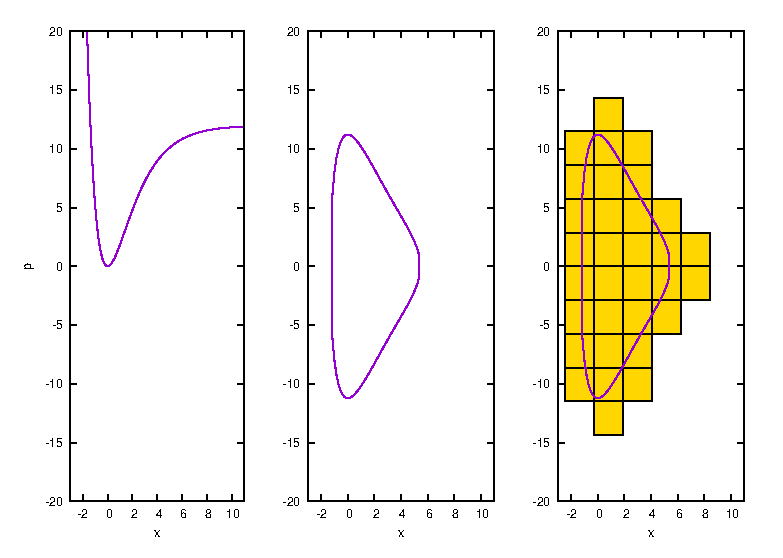
\includegraphics[width=6.5in]{morseeps}
\caption[Depiction of location of phase-space basis functions in a morse potential.]{Left) Morse potential with parameters D=12,m=6,$\beta=0.5$. Center) The classically allowed region of a Morse potential. Right) The phase space grid of functions, $g_{i,j}$ are placed at the middle of squares with area $2\pi$. } 
\label{fig.morse}
\end{figure}


The method employed by Ref.~\citenum{Halverson2012} is to form a basis using the Von Neumann lattice shown pictorially in Fig~\ref{fig.morse}. However, instead of each square occupying a area of size $2\pi\hbar$, you begin with a lattice that has square size $\pi\hbar$ and then take only symmetric combinations of $\pm p_i$ functions on the grid.    If Ref.~\citenum{Halverson2012} left the basis as a complete $\pi\hbar$ grid, it would have been overcomplete and numerically unstable.  The reason to start with this doubly dense lattice is that the critically dense lattice (namely $\Delta x\Delta p=2\pi\hbar$) is not localized once the basis functions are orthogonalized\cite{Poirier2004a}.  The necessity of localization is discussed in more detail in Chapter \ref{ch:JCP2}.


   Obtaining eigenvalues from a generalized eigenproblem generally requires orthogonalization. This is often performed by L\"{o}wdin orthogonalization.  In this case, diagonalization of the overlap matrix $S_{i,j,i^{\prime},j^{\prime}}=\int g_{i,j}\left(x\right)g_{i^{\prime},j^{\prime}}$ is performed which results in the diagonal matrix of eigenvalues $\bs{s}$ and eigenvector matrix $\bs{T}$.  One can then obtain the inverse square root of $\bs{S}$ as $\bs{S}^{-1/2}=\bs{T}\bs{s}^{-1/2}\bs{T}^{\dagger}$, The eigenvalues of the Hamiltonian can be found by diagonalizing $\bs{S}^{-1/2}\bs{HS}^{-1/2}$.  If you set up a vector $\vec{g}$ which has elements $g_{i,j}\left(x\right)$ then the vector of orthogonalized basis functions are $\bs{S}^{-1/2}\vec{g}$.  When using the critically dense vN basis, these orthogonalized functions turn out to only have inverse decay at critical density even though the individual $g_{i,j}\left(x\right)$ have Gaussian decay.  This was the motivation for starting with the doubly dense basis functions which  are
 \begin{equation}\label{eq.psdd}
 g_{i,j}=\exp\left[-A_i\left(x-
x_{n_x}\right)^2\right]\cos\left[p_{n_p}\left(x-x_{n_x}-\dfrac{dx}{2}\right)\right],
 \end{equation} 
 where due to relationships in grid spacing and $A_i$, the phase factor $\dfrac{dx}{2}$ can also be written as $\sqrt{\dfrac{\pi}{4A_i}}$.  The doubly dense functions have exponential decay which is somewhat less localized than the than the Gaussian decay of the $g_{i,j}\left(x\right)$.
 
 
 A second successful use of of Von Neumann lattice basis sets was proposed by Shimshovitz and Tannor in 2012\cite{Shimshovitz2012}.  This begins with the basis set of Eq.~(\ref{eq.wps1}) but instead of applying the Hamiltonian to Gaussians themselves, the initial Hamiltonian matrix is set up using the Fourier Grid Hamiltonian.  The Fourier Grid Hamiltonian (FGH) basis is
 \begin{equation}\label{eq.four}
\phi_n \left(x\right) = \sum_{j=-N/2+1}^{N/2}\dfrac{1}{\sqrt{LN}} \exp\left[\dfrac{i2 \pi j}{L}\left(x-x_n\right)\right],
 \end{equation}
where $x_n$ are equally spaced points in the domain $[0,L]$.  This is commonly referred to as the sinc discrete variable representation which \Refc{Shimshovitz2012} claims covers approximately the same area phase space as $N$ $g_{i,j}\left(x\right)$ basis functions with position space centres in $\left[0,L\right]$ and momentum space centres in $\left[-P,P\right]$ where $P=N dp/2$. This correspondence between the FGH and Von Neumann bases is shown for the use of 9 sinc functions and a $3\time3$ grid in phasespace.  The sinc functions are centred on the grid on the bottom while the Von Neumann basis functions are centred in the middle of the squares.
\begin{figure}[!ht]
\begin{center}
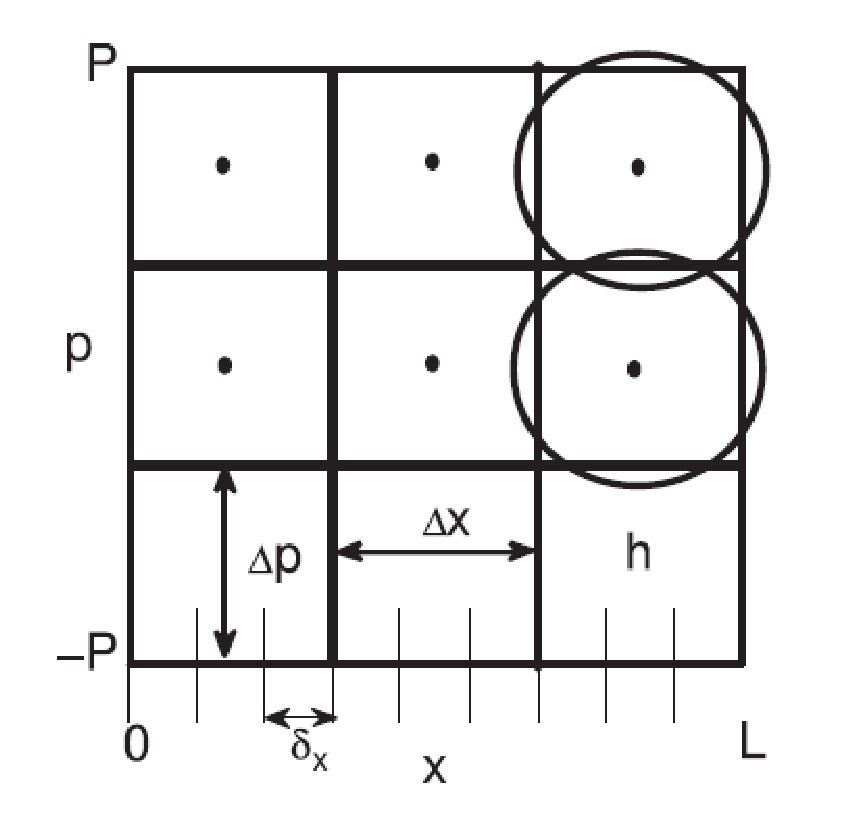
\includegraphics[scale=0.5]{shim.eps}
\caption[Pictorial of ST basis functions]{9 sinc and $3\time3$ Von Neumann basis functions. The sinc functions are centred on the dashed lines on the bottom while the Von Neumann basis functions are centred in the middle of the squares. Figure taken from \Refc{Shimshovitz2012}}
\label{fig.r4}
\end{center}
\end{figure}

 From this, the basis functions are taken to be
\begin{equation}\label{eq.psfg}
\tilde{g}_{i,j}\left(x\right)=\sum_{n=1}^{N}\phi_n\left(x_n\right)g_{i,j}\left(x_n\right).
\end{equation}
If a $G$ matrix is defined with elements $G_{k,l}=g_{l}\left(x_k\right)$, where $l$ runs over all $i,j$ values, than Eq.~(\ref{eq.psfg}) can be rewritten as $\tilde{G}=\Phi G$. Since $\int \phi_m\left(x\right)\phi_n\left(x\right)$ is diagonal, the matrix representation is
\begin{equation}\label{eq.psfg2}
H_{i,j,i^{\prime},j^{\prime}}U=
\sum_{m=1}^{N}\sum_{n=1}^{N}g_{i,j}\left(x_m\right)\left(\int \phi_m\left(x\right)H\phi_n\left(x\right)\right)g_{i^{\prime},j^{\prime}}\left(x_n\right)U=SU
\end{equation}
This basis turns out to not be conducive to pruning in that every basis function removed decreases the accuracy of the eigenvalues.  If you instead use basis functions $b_{k}\left((x\right)=\sum_{l=1}^N\tilde{g_{l}}\left(S^{-1}\right)_{l,k}$ then it results in the matrix representation
\begin{equation}\label{eq.psfg3}
H_{k,l}U=.\sum_{m=1}^{N}\sum_{n=1}^{N}b_{l}\left(x_m\right)\left(\int \phi_m\left(x\right)H\phi_n\left(x\right)\right)b_{k}\left(x_n\right)U=S^{-1}U
\end{equation}
which can be pruned without decreasing the accuracy.  

%% ****** Start of file apstemplate.tex ****** %
%%
%%
%%   This file is part of the APS files in the REVTeX 4 distribution.
%%   Version 4.1r of REVTeX, August 2010
%%
%%
%%   Copyright (c) 2001, 2009, 2010 The American Physical Society.
%%
%%   See the REVTeX 4 README file for restrictions and more information.
%%%
% This is a template for producing manuscripts for use with REVTEX 4.0
% Copy this file to another name and then work on that file.
% That way, you always have this original template file to use.
%
% Group addresses by affiliation; use superscriptaddress for long
% author lists, or if there are many overlapping affiliations.
% For Phys. Rev. appearance, change preprint to twocolumn.
% Choose pra, prb, prc, prd, pre, prl, prstab, prstper, or rmp for journal
%  Add 'draft' option to mark overfull boxes with black boxes
%  Add 'showpacs' option to make PACS codes appear
%  Add 'showkeys' option to make keywords appear





%\documentclass[aps,prl,preprint,superscriptaddress]{revtex4-1}
%\documentclass[aps,prl,reprint,groupedaddress]{revtex4-1}

% You should use BibTeX and apsrev.bst for references
% Choosing a journal automatically selects the correct APS
% BibTeX style file (bst file), so only uncomment the line
% below if necessary.
%\bibliographystyle{apsrev4-1}


% Use the \preprint command to place your local institutional report
% number in the upper righthand corner of the title page in preprint mode.
% Multiple \preprint commands are allowed.
% Use the 'preprintnumbers' class option to override journal defaults
% to display numbers if necessary
%\preprint{}

%Title of paper

\chapter{Comment on ``Phase-Space Approach to Solving the Time-Independent Schr\"{o}dinger Equation"}\label{ch:PRL}

\section{Introduction}
When reproducing the results of the ST paper of \Refc{Shimshovitz2012}, it was determined that certain inaccurate conclusions were drawn. A brief review of \Refc{Shimshovitz2012} is outlined in section \ref{sec:ps} from which is manuscript is a comment on. However, readers are encouraged to have \Refc{Shimshovitz2012} nearby. 

The following content of this chapter is the paper published as \Refc{Brown2015}.


\section{Content of Chapter}


 Shimshovitz and Tannor (ST) \cite{Shimshovitz2012} introduced a periodic von Neumann (vN) basis for solving the Schr\"{o}dinger 
equation. 
%
 Their contribution is important because it outlines ideas that make it possible to prune a vN basis.
  We   point  out that, contrary to statements of ST,  neither their  biorthogonal  pvb basis nor the periodicity of the underlying sinc functions are required
to make  a pruneable basis with which results of similar quality are obtained.  
  The first attempt to use a vN basis \cite{Davis1979} was unsuccessful.  Other approaches to 
exploiting the phase-space locality of 
vN functions  are those of \Refs{Poirier2003,Halverson2012}.

 ST use  vN Gaussians  to contract a 
Fourier grid Hamiltonian \nomenclature{FGH}{Fourier Grid Hamiltonian}(FGH) discrete variable representation (DVR) basis.
  The simultaneous diagonalization basis of \Refs{Dawes2005,Dawes2006} was used in a similar fashion to contract a harmonic basis. 
 ST begin with a pvN\nomenclature{pvN}{Periodic von Neumann} basis, 
%
\begin{equation}\label{PRLeq.1}
\tilde{g}_m\left(x\right) =\sum_{n=1}^{N}\phi_n\left(x\right)g_m\left(x_n\right)
\end{equation}
where  $g_m(x)  $ are  vN Gaussians   and   $\phi_n\left(x\right)$ are  periodic sinc functions centered at 
equally spaced points  $x_n$ and transform  the time-independent Schr\"{o}dinger equation (TISE) in the FGH  basis,
 $\bf{ H   U} = {\bf{UE}}$, 
 
%
%\begin{equation}
%\bf{ H^{sDVR}    U} = {\bf{UE}}
%\end{equation}
to obtain 
\begin{equation}
\bf{G^{\dagger} H G V} = {\bf{S V E}} ~,
\label{PRLpvnunchop}
\end{equation}
where  $G_{ij}=g_j\left(x_i\right)$,  ${\bf{S}}$ = ${\bf{G^{\dagger} G}}$   and ${\bf{U}}$ = ${\bf{GV }}$.   
%
ST propose transforming to a pvb basis, 
\begin{equation}
\bf{S^{-1} G^{\dagger} H G S^{-1}  Z} = {\bf{ S^{-1}    Z E}} ~,
\label{bvnunchop}
\end{equation} 
where ${\bf{Z}}$ = ${\bf{S V }}$. 
Both \Eq{PRLpvnunchop} and \Eq{bvnunchop} are generalized eigenvalue problems of the form 
\begin{equation}
\bf{AY } = {\bf{ BYL}}~.
\label{genform}
\end{equation}  
%
The pruned pvN eigenvalue problem is $\bf{     C^{\dagger}G^{\dagger} H  GCV}  =   \bf{C^{\dagger}SCV \tilde{E}}~$,
%\begin{equation}\label{eq.2}
%\bf{     C^{\dagger}G^{\dagger} H^{sDVR} GCV}  =   \bf{C^{\dagger}SCVE}~, 
%\end{equation}  
 where ${\bf{C}}$ has  $n_k$  diagonal elements equal to   one  and $n_d=N-n_k$  elements equal to zero.  Matrices  playing
 the role of $both$  ${\bf{A }}$  and $ {\bf{ B}}$,  in \Eq{genform}    are chopped.
Pruning  the pvN  basis significantly degrades the accuracy of the energies.   
%
The pruned pvb eigenvalue problem is 
%
\begin{equation}\label{PRLeq.3}
	\bs{C^{\dagger}S^{-1}G^{\dagger} H  GS^{-1}CU}=\bs{C^{\dagger}S^{-1}CU \tilde{E}},
\end{equation}   
and in this basis, it $is$  possible to prune and maintain accuracy!
Again,    
the matrices playing  the role of $both$  ${\bf{A }}$  and $ {\bf{ B}}$  are chopped.   





There is, however,  no need to introduce the pvb basis.   Starting with \Eq{PRLpvnunchop},  moving ${\bf{S}}^{-1}$ to the left and $then $
pruning, one obtains the nonsymmetric eigenvalue problem 
\begin{equation}\label{our}
\bf{C^{\dagger}  S^{-1}  G^{\dagger} H^{DVR} G  CV}={\bf{V  \bar{E}}}.
\end{equation} 
%
It is easier to solve    Eq (\ref{our}) than \Eq{PRLeq.3}   with    iterative eigenvalue solvers  
 because  it is not a generalized eigenvalue problem
(therefore larger systems are accessible).  
%\cite{Bai2000}
%tc this is   Z. Bai, J. Demmel, J. Dongarra, A. Ruhe and H. van der Vorst, editors, 
%Templates for the solution of Algebraic Eigenvalue Problems: A Practical Guide . SIAM, Philadelphia, 2000
%  
For the 1D Morse potential of  Ref. \citenum{Shimshovitz2012},  we compare eigenvalues computed with   \Eq{our}   and \Eq{PRLeq.3},
using  $N=196$ initial basis functions. 
%
In both cases, the error does not 
decrease until about $n_k = 98$.   
 %Thus,  the pvN basis,  truncated using    \Eq{our},  has   most of the advantages of the pvb basis.  
%  The most important idea is to use 
%Gaussians to contract rather than to use them as basis functions.  
%
 \begin{figure}[ht]
 \includegraphics[width=6.5in]{PRL/fig_1ab.eps}%
 \caption[Comparison of different methods for the 22nd eigenvalue of the Morse oscillator]{The error of the 22nd eigenvalue of the Morse oscillator
\label{PRLfig.1} a) Comparison of ST's pvb with the FGH and \Eq{our} with the Colbert and Miller (CM)\cite{Colbert1992} Sinc DVRs. %JB24
   b) Comparison of Hermite (H$_n(x)$) and Legendre (P$_n(x)$) DVRs using \Eq{our} and ST's pvb.}
 \end{figure}
%


According to  ST, the accuracy of the \Eq{PRLeq.3} levels  is due in part  to the
 periodicity of the  sinc DVR.  We have confirmed that with  \Eq{our}, energies obtained with 
non-periodic DVRs \cite{Light2000}  are also accurate; see  Fig. \ref{PRLfig.1}b  for the Morse oscillator of ST. 
 Fig. \ref{PRLfig.1}b is  generated with   vN  functions 
  at $\sqrt{N}$ position values $x_i$ that are  a subset of the    DVR  points. %,  
%
After sending this comment to ST,   we learned that they had done pvb calculations with other DVRs.   \cite{Shimshovitz2014b}  
The fact that both  \Eq{our} and the ST approach work with other DVRs  is clearly incompatible with 
 the assertion  that periodicity is important.  
% 
% When $n_k$ is small the pvN energies are, however, more accurate.  
 %We have  done similar calculations with other potentials.  
%It might be possible to choose the vN parameters  to improve the accuracy.   
%
Knowing that the ST idea of contracting with Gaussians can be applied to other DVRs opens the door to using it to solve many problems
for which      sinc DVRs are not ideal.  
 %Legendre DVRs are well suited to solving problems in polyspherical coordinates.   %Legendre matrix elements of 
%the    polyspherical kinetic energy operator are well known. 
%
% 
%



In summary, it  is not necessary to think in terms of the  pvb basis ST  introduce if the pvN eigenproblem is truncated as in \Eq{our},   and 
 the contraction idea ST use   enables one to use Gaussians to contract any DVR basis. %JB25
%


% If in two-column mode, this environment will change  to single-column
% format so that long equations can be displayed. Use
% sparingly.
%\begin{widetext}
% put long equation here
%\end{widetext}

% figures should be put into the text as floats.
% Use the graphics or graphicx packages (distributed with LaTeX2e)
% and the \includegraphics macro defined in those packages.
% See the LaTeX Graphics Companion by Michel Goosens, Sebastian Rahtz,
% and Frank Mittelbach for instance.
%
% Here is an example of the general form of a figure:
% Fill in the caption in the braces of the \caption{} command. Put the label
% that you will use with \ref{} command in the braces of the \label{} command.
% Use the figure* environment if the figure should span across the
% entire page. There is no need to do explicit centering.

% \begin{figure}[h!]
% \includegraphics[scale=0.4]{fig_1ab.eps}%
% \caption{The error of the 22nd eigenvalue of the Morse oscillator
%\label{fig.1} a) Comparison of ST's pvb  and \Eq{our}.   b) Comparison of three different DVRs using Eq (\ref{our}).}%JBnew added reference to Eq (7)
% \end{figure}

% Surround figure environment with turnpage environment for landscape
% figure
% \begin{turnpage}
% \begin{figure}
% \includegraphics{}%
% \caption{\label{}}
% \end{figure}
% \end{turnpage}

% tables should appear as floats within the text
%
% Here is an example of the general form of a table:
% Fill in the caption in the braces of the \caption{} command. Put the label
% that you will use with \ref{} command in the braces of the \label{} command.
% Insert the column specifiers (l, r, c, d, etc.) in the empty braces of the
% \begin{tabular}{} command.
% The ruledtabular enviroment adds doubled rules to table and sets a
% reasonable default table settings.
% Use the table* environment to get a full-width table in two-column
% Add \usepackage{longtable} and the longtable (or longtable*}
% environment for nicely formatted long tables. Or use the the [H]
% placement option to break a long table (with less control than 
% in longtable).
% \begin{table}%[H] add [H] placement to break table across pages
% \caption{\label{}}
% \begin{ruledtabular}
% \begin{tabular}{}
% Lines of table here ending with \\
% \end{tabular}
% \end{ruledtabular}
% \end{table}

% Surround table environment with turnpage environment for landscape
% table
% \begin{turnpage}
% \begin{table}
% \caption{\label{}}
% \begin{ruledtabular}
% \begin{tabular}{}
% \end{tabular}
% \end{ruledtabular}
% \end{table}
% \end{turnpage}

% Specify following sections are appendices. Use \appendix* if there
% only one appendix.
%\appendix
%\section{}



\chapter{Using an iterative eigensolver to compute  vibrational energies with phase-spaced localized basis functions\label{ch:JCP1}}
\thispagestyle{empty}

\section{Introduction}
This chapter applies the knowledge obtained from manuscript 1 of the previous chapter to the H$_2$O molecule.  It also discusses in detail the theoretical understanding of why the ST method works. 

The following content of this chapter is the manuscript published as \Refc{Brown2015b}.

\section{Abstract}
% 
Although phase-space localized  Gaussians are themselves poor basis functions, they 
 can be used to effectively contract a discrete variable representation basis (A.  Shimshovitz and D. J. Tannor, Phys. Rev. Lett. 109, 070402 (2012))
  This works despite the fact that elements of the 
Hamiltonian  and overlap matrices labelled by discarded Gaussians are not small.  
By formulating the matrix problem as a regular (i.e. not a generalized)     matrix eigenvalue problem
we show that it is possible to use 
 an iterative eigensolver to compute vibrational energy levels in the Gaussian basis.


  


% body of chapter here - Use proper section commands
% References should be done using the \cite, \ref, and \label commands
\section{Introduction}


The most general and systematic way to solve the Schr\"{o}dinger equation is to represent   wavefunctions in a basis and use  methods of numerical
linear algebra to determine coefficients.  For example, to solve a 1D  time-independent Schr\"{o}dinger equation\nomenclature{TISE}{Time Independent Schr\"{o}dinger Equation} (TISE), one uses a basis $   \theta_k(x) $
\begin{equation}  
\psi(x) = \sum_k  c_k  \theta_k(x)
\end{equation}
and solves for the $  c_k $.   Frequently,  the    $  c_k $ are determined by multiplying on the left by    $ 
 \theta^*_j(x)$ and integrating to obtain a matrix eigenvalue equation.\cite{Carter1986,Tennyson1986,Sibert1990,Bacic1989,Bowman2008}     
%
It is often difficult to implement this procedure
 to compute  solutions of  the Schr\"{o}dinger equation, from which  vibrational spectra, 
photodissociation cross sections, rate constants etc, are calculated  because
the size of common basis sets 
scales exponentially with the number of coordinates 
($3N-6$, where $N$ is the number of atoms, for a $J=0$ calculation).    



The basis is huge in part because quantum mechanics is non-local.  However, it is clear that standard direct product basis sets, although 
they may facilitate calculations, are much larger than they need to be.   One way to make  a  smaller basis that is adequate for the purpose of 
computing vibrational spectra is to use products of eigenfunctions of reduced-dimension Hamiltonians. 
%
  This contraction idea is sometimes used  with adiabatic-like
functions.\cite{Bacic1989,Henderson1990,Bowman1991,Qiu1998,Mladenovic2002a,Mladenovic2002b,Luckhaus2000}  
 In this case,  a set of basis functions for one group of coordinates is  calculated for each of  many values of the other coordinates.  
Contraction can also be done with ``simply contracted functions''\cite{Carter1988,Bramley1994b}  
 by computing a single set 
 of basis functions for one group of coordinates   for one value  of the other coordinates.\cite{Koput2001,Wang2002,Yu2002,Wang2004,Yu2002b,Tremblay2006,Lee2003} % 
In this chapter we develop and apply a very different contraction strategy.   It is related to the work of Davis and Heller\cite{Davis1979} (DH),  
 of Poirier and co-workers,\cite{Poirier2003,Poirier2004a,Poirier2004b,Halverson2012,Halverson2015}  and of  Tannor and co-workers.\cite{Shimshovitz2012,Shimshovitz2014}  
 %
%
The key idea is that  an efficient basis is one whose phase space representation covers the same region as the wavefunctions one wishes to compute.  This idea
motivated the early work of DH, and is clearly expressed in \Refc{Poirier2000} where Poirier discusses the Wigner representation of a basis.    
%


The simple idea of using basis functions (whose Wigner representation is) localized in phase space is intuitive and attractive.    It should enable us 
to use knowledge extracted from classical mechanics to design an efficient basis.   One expects that a basis covering  (in the Wigner sense) 
a region slightly larger than the classical region 
of phase space should be sufficiently large for the purpose of computing accurate wavefunctions.    
For several decades scientists have pursued the hope that such a classically-motivated basis would be useful    
%
%
\cite{Davis1979,Poirier2000,Poirier2003,
Poirier2004b,Poirier2004a,Dawes2005,Dawes2006,Halverson2012,Shimshovitz2012,Shimshovitz2014,Halverson2015}.
 DH were the first to apply this idea in chemical physics.\cite{Davis1979} 
 They used a 1D von Neumann (vN) basis on a grid with each function corresponding to a phase space area of  size   $h$.     
Their approach worked surprisingly poorly.   If the area per basis function is reduced and the size of the basis is increased, it is sometimes possible
to  obtain accurate results.    
%
However, in many cases as the basis size is increased (and the ``area'' per function is decreased), 
near linear dependence of the basis becomes so severe that it is not possible to compute accurate energy levels.
%
%  increasing the basis size
%(and decreasing the ``area'' per function) because numerical problems, arising from the near linear dependence, impede solution of the matrix eigenvalue problem.   


Poirier and co-workers introduced new ideas for mitigating  the deficiencies of the DH approach. 
 In one set of papers,\cite{Poirier2003,Poirier2004b,Poirier2004a} they define orthonormal Weylets and show that  
it is possible to use a relatively small number of  Weylets  and compute accurate energies. 
 There is no problem with near linear dependence because the 
basis is orthonormal.
%
    In another set of papers, they use a symmetrized Gaussian basis and solve a generalized eigenvalue problem.\cite{Halverson2012,Halverson2015}   Also
in this approach,  there is no problem with near linear dependence.   
%
%
%
Dawes and Carrington used a simultaneous diagonalization\nomenclature{SD}{Simultaneous Diagonalization} (SD) algorithm to make 1D wavelet-like orthogonal basis functions  and showed that for many dimensional problems it possible to calculate
accurate energies by pruning the basis formed by making 
 products of the 1D SD  functions products.\cite{Dawes2005,Dawes2006}
%
 Shimshovitz and Tannor\nomenclature{ST}{Shimshovitz and Tannor} (ST) \cite{Shimshovitz2012} introduced a ``periodic von Neumann with biorthogonal exchange''\nomenclature{pvb}{periodic von Neumann with biorthogonal exchange} (pvb) basis for solving the TISE.   ST begin with a discrete variable representation \cite{Light1985,Bacic1989,Light2000} (DVR) 
%
  of the Hamiltonian, transform to the pvb basis, prune the pvb basis, and solve a generalized
eigenvalue problem.  
%


Our  chapter reports progress on  two  fronts.  
 %(1) We demonstrate that it is possible to discard (finite representations of) vN functions.  
%
(1) We explain in detail when, and why  discarding vN\nomenclature{vN}{von Neumann} basis functions works, despite the fact that the  corresponding (e.g. Hamiltonian) matrix elements are not small.  
(2)  We  show that an iterative eigensolver can be used to solve a vN matrix eigenvalue problem.   To do this, it is essential to formulate the 
problem as a regular (i.e. not a generalized)     matrix eigenvalue problem.
Because  the matrix eigenvalue problem we solve  is not generalized (i.e. no overlap matrix on the right side multiplying the matrices of 
eigenvectors and eigenvalues),  it is 
 possible,   to use an iterative eigensolver and hence avoid storing  large matrices.
%tc changes .  please take the time to check this.    please sort the references.  please make sure cite(old) appears in the list.  
%  
Poirier and co-workers have shown that   phase-space localized basis  methods can be applied to polyatomics        without   iterative  eigensolvers.    Recently this has been achieved by using  massive computers, 
as methods of direct linear algebra, which require storing matrices,  are used to solve eigenproblems with matrices whose size is $~ \sim 10^5$.  
\cite{Halverson2012,Halverson2015}
%
In an  older paper,  using much less computer power,   
Poirier applied his   ideas to compute levels of a  15D  isotropic harmonic oscillator with unit frequency.
\cite{Poirier2003}
%
   The  percentage error criterion used   in \cite{Poirier2003}  and  explained in    \Refc{Poirier2004b}   is 
$\delta_{wavelet}= [100 (E_{eiv}- E_{exact})]/(10 D)$,  where  $D$ is  the dimensionality and   $ E_{eiv}$ is the computed eigenvalue.
%
 When  $\delta_{wavelet}= 2$,  absolute errors are large, e.g. when $D=15$ and   $E_{exact}=7.5$ (the energy of the ground state)  
the  absolute error is   3.           
Lombardini and Poirier have used a subspace iteration iterative method with their Weylets.  \cite{Lombardini2006}    This is done for model problems  by exploiting sparsity.  
Iterative eigensolvers obviate the need to store matrices, and thus greatly reduce the cost of computing energy levels of interest.\cite{Bai2000} 


















\section{Using a von Neumann basis }\label{sec:BC}

In this section we present and analyse several ways of using a von
Neumann basis.   Subsection \ref{sseca} is devoted to the original DH approach.  Rather
than using the vN functions as basis functions they can be used to 
contract a DVR basis. \cite{Halverson2012}  This can be thought of as a basis transformation.     This idea is  introduced in subsection \ref{ssecb}.  In subsection \ref{ssecb} we explain 
that some basis transformations yield a pruneable matrix and others do not.   The eigenvalue problem is pruneable if rows of the matrix of eigenvectors can be discarded.  
In subsections \ref{ssecc} and \ref{ssecd},   we compare the two projection strategies.


\subsection{Projecting $\hat{H}$  into a vN basis}\label{sseca}


%tc no link  between eq 2 and first clause.   tc changed %JB looks good
%Start with some 
%huge vN basis  % removed  whose size and parameters make it possible, in principle, to solve the TISE,
%\begin{equation}
%\hat{H} \psi_n(x) = \epsilon_n \psi_n(x)   ~.
%\end{equation}
%In the huge   vN basis  the   eigenvalue problem is 
%\begin{equation}
%\bf{  H_G W} = {\bf{S_G W  E}} ~,
%\label{full}
%\end{equation}
%
Start by representing 
\begin{equation}
\hat{H} \psi_n(x) = \epsilon_n \psi_n(x)   ~.
\end{equation}
in a huge vN basis 
to obtain 
  the   eigenvalue problem 
\begin{equation}
\bf{  H_G W} = {\bf{S_G W  E}} ~,
\label{full}
\end{equation}
where ${ ( \bf{  H_G }   )}_{m',m}$    
 $ = \langle  g_{m'} \vert \hat{H}  \vert g_m \rangle     $,
%
${ ( \bf{  S_G}   )}_{m',m}$    $ = \langle  g_{m'} \vert  g_m \rangle     $, $m',m  = 1, \cdots F$, and   
 \\  $g_{m(i,j)}(x)=\exp\left[-\alpha_i\left(x-x_i\right)^2 + i p_j\left(x-x_i\right)\right]  $ is a   vN Gaussian   
 centered at $(x_i,p_j)$ with width parameter $\alpha_i$.  
%
%
In \Eq{full}   $ {\bf{  W} }   $ is a  matrix containing the eigenvectors and 
 $ {\bf{  E} }   $ is a diagonal matrix whose nonzero elements are the eigenvalues.   
One hopes that it is possible 
   discard some of the basis functions (prune the basis) without degrading the accuracy of the eigenvalues.  
%
DH replace \Eq{full} with 
\begin{equation}
\bf{  H^c_G W^c} = {\bf{S^c_G W^c  E^c}} ~,
\label{davis}
\end{equation}
where,  like   ${   \bf{  H_G}}$  and $  {\bf{S_G }}$,    $({\bf{  H^c_G }})_{m',m}    = \langle  g_{m'} \vert \hat{H}  \vert g_m \rangle   $ 
and ${ ( \bf{  S^c_G}   )}_{m',m}$    $ = \langle  g_{m'} \vert  g_m \rangle     $, but 
with $m',m  = 1, \cdots N_k$.  Thus, $N_k$ is the size of the chopped matrix. 












\subsection{Projecting    $ {\bf{ H}}$ into a vN basis}\label{ssecb}

%

Instead of using the $g_{m}$ as basis functions,    one can  use   them 
 to contract some other basis.\cite{Shimshovitz2012}
   To do this, begin   by projecting the TISE into 
some real finite orthonormal basis (a discrete variable  representation 
  \cite{Light1985,Bacic1989,Light2000} 
basis is convenient) whose $N$ functions are denoted
 $\phi_\alpha(x)$,
\begin{equation}  
\bf{ H U} = {\bf{U \tilde{ E}}} ~.
\label{dvrmateiv}
\end{equation}
 The  goal is now to find a basis of finite-dimensional $vectors$ in which one 
 can represent columns 
of ${\bf{  U}}$.   
 This is not the same as finding a basis of $functions$
with which we can represent $\psi_n(x)$.
% 
We introduce   $ \bf{  U} = {\bf{ G A   }}  $, where   $ {(\bf{  G}})_{\alpha,m} $ = $ \langle \phi_\alpha  \vert     g_m   \rangle $ are elements of a square
%
transformation matrix.  One obtains, 
%
\begin{equation}
\bf{G^{\dagger} H G A} = {\bf{S A \tilde{E}}} ~,
\label{pvnunchop}
\end{equation}
where  $\bf{ S} = {\bf{  G^{\dagger}  G }}$.
%
%
%
%
%
%
%\begin{equation}\label{eq.1}
%\tilde{g}_m\left(x\right) =\sum_{\alpha=1}^{N}   \langle   \phi_{\alpha} \vert g_m \rangle     \phi_{\alpha}\left(x\right)     ~.
%\Eq{gtilde}
%\end{equation}
The $ {\bf{ H }}  $ used in the original 
ST   paper was the Fourier grid Hamiltonian\cite{Marston1989}
%
  and their   $\phi_{\alpha}(x)  $ were 
  periodic Fourier-Grid-Hamiltonian (FGH)  functions,   but other DVRs can also be used.\cite{Brown2015,Shimshovitz2014}
%






%
The matrices in     \Eq{pvnunchop} are  as large as  $ { \bf{  H  }}$.  To make the transformation  useful one must prune the basis, i.e. reduce the number of 
vN functions from $N$ to $N_{k}$.   
%
As explained by ST, if this is done by retaining only selected  rows and columns      of  both    $ \bf{G^{\dagger} H G }$
  and  $ {\bf{S}}$,   eigenvalues of the pruned problem differ significantly from those of   \Eq{pvnunchop}. \cite{Shimshovitz2012}
%
       In terms of symbols, 
$ \bf{ \tilde{{\bar{E}}}}$ differs significantly from   $ \bf{ \tilde{{{E}}}}$, where 
 ${\bf{     C^{\dagger} G^{\dagger} H  GC A_c} } =   {\bf{C^{\dagger}S C A_c  \tilde{{\bar{E}}}}}~$,
and 
  ${\bf{C}}$ is a diagonal matrix with  $N_{k}$  % (the number of retained   basis functions) 
diagonal elements equal to   one  and $N_d=N-N_{k}$ (the number of discarded  basis functions) 
 elements equal to zero.  When a matrix is multiplied on the right by ${\bf{C}}$,  
some of its columns are set to zero.



%
%
In general, prune-ability can be achieved by  replacing   ${\bf{G}}$    
 with a matrix ${\bf{T}}$ and \Eq{pvnunchop}  with   
 ${\bf{     T^{\dagger} H  T  X} } =   {\bf{      T^{\dagger}   T  X     {{\tilde{E}}}}}~$, 
and  choosing  ${\bf{T}}$ so that  
  ${\bf{     (  T^{\dagger}   T   )^{-1}    T^{\dagger} H  T }}$ 
%
(or     ${\bf{        T^{\dagger} H  T   (  T^{\dagger}   T   )^{-1}   }}$  or \\*
${\bf{       (  T^{\dagger}   T   )^{-1/2} T^{\dagger} H  T   (  T^{\dagger}   T   )^{-1/2}   }}$)    
is nearly diagonal. % 
%
There is another way. 
%
Choose a new basis and the corresponding transformation matrix  ${\bf{   T  }}$   so that 
  ${\bf{  U = T X }}$, 
 ${\bf{        T^{\dagger} H  T     X =    S_T X \tilde{E} }}$, 
and ${\bf{        T^{\dagger} H  T^{-\dagger}        Y =  Y \tilde{E} }}$  , 
%
 where ${\bf{   S_T=   (  T^{\dagger}   T   )    }}$  and  ${\bf{      T^{-\dagger}    =   (T^{\dagger})^{-1}  }}$,    and choose 
  ${\bf{         T    }}$ 
so that  the desired portion of 
  ${\bf{    Y =    T^{\dagger}   U  }}$  has  rows that  are tiny.
When such a basis can be found, 
   it is possible to remove rows and columns of    ${\bf{        T^{\dagger} H    T^{-\dagger}        }}$       without jeopardizing
the  accuracy of the desired eigenvalues.      
To explain why this is true,  define  $ { \bf{ M  =     T^{\dagger} H  T^{-\dagger}     }}$, and $  \bf{ {\tilde{M}}}$ which is 
obtained by   replacing the $N_{k}$ elements,  that correspond to retained  basis functions,   of each of  the  $N_d$  %$N-N_{k}$ 
columns of  $ { \bf{ M }}$ that correspond to discarded basis functions, with zeros. 
If the retained and discarded rows and columns are grouped together then the retained-discarded corner of  
$  \bf{ {\tilde{M} }} $   is zero, and therefore the desired eigenvalues and eigenvectors of $  \bf{ {\tilde{M} }} $ are exactly equal to 
 eigenvalues and eigenvectors of the retained corner of $  \bf{ {\tilde{M} }} $  and 
 are nearly equal to eigenvalues  
 and eigenvectors of the retained-retained corner of $  \bf{ {{M} }} $.
%
%
%


One option is to choose  $\bf{ T } = {\bf{    G^{-\dagger}   }} $.
%
This choice of $\bf{T}$ is equivalent to beginning with \Eq{pvnunchop} and multiplying on the left by ${\bf{S^{-1}}}$, as ${\bf{S^{-1}G^{\dagger}}=\bf{G^{-1}}}$.
  One then  obtains 
%
\begin{equation}
\bf{  G^{-1}   H G A} = {\bf{ A \tilde{E}}} ~,
\label{Avecs}
\end{equation} 
where   $ {\bf{  Y}}  $  in the previous paragraph is replaced by    $ {\bf{  A}}  $;
  $ {\bf{  A= G^{-1}  U }}  $.       
If   $A_{m,n}  $  were small  for some $m$,  then it would   be possible to discard
rows and columns of  $
\bf{  (G^{-1})  H G }$.      Does one expect 
  $A_{m,n}  $  to be small for some $m$?
%
%
%
%
%
%To compute  the $n$th column  of  ${\bf{ A }}$    , one can discard   rows of    $\bf{ G^{-1}}$  for which 
%  entries of large  magnitude  only occur in columns 
% that correspond to  
% entries of  ${\bf{ U}}_n$                     ( ${\bf{ U}}_n$ is 
%a  column of   $ {\bf {U}} $)
%of small  magnitude.    
%
%
The $m$th element of  the $n$th column  of  ${\bf{ A }}$  is small if
the  entries of large  magnitude  of the $m$th row of 
   $\bf{ G^{-1}}$   only occur in columns   that correspond to   entries of  ${\bf{ U}}_n$                     ( ${\bf{ U}}_n$ is 
a  column of   $ {\bf {U}} $) of small  magnitude.    
%
However, in general,  there   
 is no reason to expect some rows of $  \bf{ G^{-1}}  $   to have large magnitude   elements only for  $\alpha$  values for which     $ {\bf {U}}_{\alpha,n} $ is small.  
%
%
It is therefore not obvious that   rows and columns can be  removed from ${
\bf{  (G^{-1}) H  G }}$.
% 


%
%
Another option is to choose        ${\bf{ T }}$    =       ${\bf{ G }}$
%  
%
to  obtain the eigenvalue problem
 $  {\bf{G^{\dagger} H G^{-\dagger}     B}}= {\bf{B  \tilde{E}}} $, where
in this case  ${\bf{ Y }}$  is replaced by    ${\bf{ B }}$  and   ${\bf{ B }}$  =  ${\bf{G^{\dagger} U }}$.   
%
%
If no rows and columns are removed,  the eigenvalues are equal to those obtained from the  pvb formulation of ST,
 but in the pvb basis one must solve    a generalized eigenvalue problem.   
  Is there reason to believe that rows of the desired portion of  ${\bf{B}}$ may be small?     
% 
 When  the $ \phi_{\alpha}$ basis is a DVR basis,    the $m$th element of the $n$th column of ${\bf{B}}$ will be small if in 
 the $m$th row of   $ \bf{G^{\dagger}}$   
   the only large magnitude elements  
 correspond to   $ \vert g_m(x_{\alpha} ) \vert  $ values 
for     which the magnitude of 
 $\psi_n(x_{\alpha})$ is small.   
%
%
  There are such rows    because the 
$  {g_m} $ functions and the wavefunctions  are localized in position space.\cite{Shimshovitz2014,Tannor2014} 
%
%
 The $m$th element of the $n$th column of ${\bf{B}}$ will  be small 
whenever  ${\bf{G}}_m^{\dagger}   {\bf {U}}_{n} $ is small.   This can happen even if in  
  row  ${\bf{G}}_m^{\dagger}$  of  ${\bf{G}}^{\dagger} $    elements of large magnitude    correspond to large elements   $ \vert  {\bf {U}}_{\alpha,n} \vert $.  It 
%
  occurs, for example,  when 
a vN  Gaussian is highly oscillatory (i.e. large $p_j$) in a region in which 
 $\psi_n\left(x_{\alpha}\right)$ is relatively flat.  
%
Some  rows of the desired portion of ${\bf{B}}$   are small  because both   
 the vN Gaussians and the wavefunctions are    localized in momentum space.   
%
For these reasons, and because 
 $  {\bf{G^{\dagger} H  G^{-\dagger}     B}}$
= ${\bf{B  \tilde{E}}} $ is not a generalized eigenvalue problem,  it should be possible to 
remove columns and rows of     $  {\bf{G^{\dagger} H  {G^{-\dagger} }}}$    without significantly altering  the desired  eigenvalues.   
%
The pruned  eigenvalue problem obtained from  
 $  {\bf{G^{\dagger} H  G^{-\dagger}     B}}= {\bf{B  \tilde{E}}} $
 is 
\begin{equation}
\bf{C^{\dagger} G^{\dagger} H  G^{-\dagger}    C B_c}=\bf{  B_c \widetilde{E^B_c}},
\label{pruneB}
\end{equation}   
%
%$   {\bf{  B_c}}$ is obtained from $   {\bf{  B}}$ by removing rows.  
%
Note that pruning     $  {\bf{G^{\dagger} H  {G^{-\dagger} }}}$   by  removing rows of   $  {\bf{G^{\dagger} }}$ and pruning 
 $  {\bf{G^{-1} H  G }}$  
 by    removing rows of   $  {\bf{G^{-\dagger} }}$  correspond to removing different   vN functions.  
%
The  desired  eigenvalues of \Eq{pruneB} are close to those of the un-pruned problem.     \Eq{pruneB} is used in Section \ref{sec:h2o}.     











As explained after \Eq{Avecs}, one does not necessarily expect some rows  of the desired portion of $ { \bf{    A} }$,
 where 
 $  \bf{    G^{-1} H    G    A} = {\bf{ A \tilde{E}}} $ to be small.  Therefore,  it is not clear that eigenvalues of the corresponding pruned problem, 
\begin{equation}
 \bf{C^T     G^{-1} H    G     C A_c} = {\bf{ A_c \widetilde{E^A_c}}}
\label{pruneA}
\end{equation}
  will be nearly equal to those of the un-pruned problem.   
To prune  \Eq{pruneB}  (\Eq{pruneA}) one must identify small   rows of the  desired portion of   ${\bf{B}}$ (${\bf{A}}$).  
%
The gap between small and not small is larger for ${\bf{B}}$ than for ${\bf{A}}$, however, 
similar   results are  obtained  by pruning the basis vectors that correspond to the smallest  rows of 
$\bf{A}$ and ${\bf{B}}$.   They are similar  because 
eigenvalues of the transpose of a matrix are equal to eigenvalues of the matrix and 
%
  most of the removed rows of   $ { \bf{    G^{-1} }} $ correspond to removed  rows of    $ { \bf{    G^{-\dagger} }} $
%



All of the ideas of this subsection are built on the suggestion  of ST that it is best to first project into a finite (DVR) basis and only afterwards to 
discard vectors that correspond to vN functions.   A fundamental difference between our approach and ST's is that we formulate the solution as  a regular eigenvalue
problem,
 $  \bf{ M Y } = {\bf{ Y  \tilde{E} }} ~    $.   
This makes using iterative eigensolvers practical.
%
   Whenever rows of the desired portion of the matrix of  eigenvectors are tiny,  rows and columns of  $ { \bf{ M  }}  $
can be discarded, regardless of the size of the elements.  Tiny here refers to being orders of magnitude smaller than the kept rows of the matrix of eigenvectors. 
   The approach of ST  also  works, although they (separately) prune  two matrices  and solve a generalized eigenvalue problem.   Why does the ST 
approach work?   ST solve   
%JB changed X^ST to B^ST below, also added _c after chopping
  $  {\bf{   { S^{-1}  G^{\dagger} H G        S^{-1} B^{ST} =   S^{-1} B^{ST} \widetilde{E^{ST}}}}}$.  Although when all matrices are $ N \times N$, it is clear that ${\bf{\widetilde{E^{ST}}}} ={  
 \bf{\widetilde{E}}} $, it is not obvious,  after pruning to obtain 
 $  {\bf{ C^T  { S^{-1}}    G^{\dagger} H G  { S^{-1}} C  B_c^{ST}}}= {\bf{ C^T   S^{-1}  C   B_c^{ST}  \widetilde{E_c^{ST}}}} $, that $
   {\bf{\widetilde{E_c^{ST}}}} \approx   {\bf{\widetilde{E_c^{B}}}}$. 
%where   ${\bf{C^T G^{\dagger} H     G^{-\dagger}   S^{-1}     C B_C = B_C  \widetilde{E_C^{B}} }} $. 
   It is true because (1) columns of 
$ { \bf{ B^{ST}  }}  $ are proportional to columns of $ { \bf{ B  }}  $ and therefore  the desired portion of  $ { \bf{ B^{ST}  }}  $ has  $N-N_{k}$ rows with tiny  elements;
 (2)  
when solving         $  {\bf{   { S^{-1}  G^{\dagger} H G        S^{-1} B^{ST} =   S^{-1} B^{ST} \widetilde{E^{ST}}}}}$   % $\bf{        X = BXE}$, 
both $ { \bf{( B^{ST})^{\dagger}  S^{-1}  G^{\dagger} H G        S^{-1}
       B^{ST}  = \Lambda_1  }}  $   and 
 $ { \bf{   (B^{ST})^{\dagger}    S^{-1}    B^{ST}     = \Lambda_2 }}  $  are diagonal, where
 $ { \bf{ \widetilde{E^{ST}}=  \Lambda_1  {\Lambda_2}^{-1}  }}  $,
%
and therefore    replacing the 
elements of
 $ { \bf{   S^{-1}  G^{\dagger} H G        S^{-1} }}  $   and  $ { \bf{     S^{-1}   }}$
%
whose row and  column indices correspond to the   $N-N_{k}$ 
discarded basis vectors, 
with zeros, has almost no effect on $N_{k}$  eigenvalues.  Note that this does not mean that elements replaced by zeros are small.   


  
Another difference between the approach of Refs. \citenum{Shimshovitz2012}
and \citenum{Shimshovitz2014}   
is the definition of  ${\bf{ G  }}$.   We define    $ {(\bf{  G}})_{\alpha,m} $ = $ \langle \phi_\alpha  \vert     g_m   \rangle  $   and ST define 
$ {(\bf{  G^{ST}}})_{\alpha,m} $ = $   g_m(x_{\alpha}) $.   $ {(\bf{  G}})_{\alpha,m}  \ne   $ $ {(\bf{  G^{ST}}})_{\alpha,m} $  because DVR functions depend, in general,  on 
quadrature weights and a weight function.
\cite{Light1985,Bacic1989,Wei1994,Light2000} 
%
%
If the weights are all equal the difference between 
 $ {(\bf{  G}}) $ and     $ {(\bf{  G^{ST}}}) $ is unimportant.   
In general,  
 $ {(\bf{  G}})_{\alpha,m} $ =  $
 \sqrt{W^{(N)}_{\alpha}/w(x_{\alpha})} g_m(x_{\alpha}) $,
where  $W^{(N)}_{\alpha}$ is a quadrature weight and $w(x)$ is the weight function of the polynomials used to define the DVR.   Defining  $ {(\bf{  G}})_{\alpha,m} $  as we do,
 ${\bf{ G^{\dagger} V^{DVR} G     }} $ is a quadrature approximation to 
 $  \langle  g_{m'} \vert \hat{V}  \vert g_m \rangle     $.    
Including the weights   
decreases the size of the elements in the desired portion of  
 ${\bf{ B   }} $  that correspond to vN functions one wishes to discard and therefore improves the quality of the pruned basis.  
%
%
It is possible to attain pruneability with $any$ basis for which 
rows of  $  {\bf{T^{\dagger}}}$  are not nearly linearly dependent and for which 
multiplying 
rows of $  {\bf{T^{\dagger}}}$  by columns of $  {\bf{U}}$ yields small numbers.  
 This will be the case  for any DVR basis.  There is no periodicity requirement.\cite{Brown2015}





\subsection{ Comparison of projecting   $\hat{H}$   and projecting     $  {\bf{  H  }}$   }\label{ssecc} 




%
Why does using  a basis of non-orthogonal $ {g}_m $ functions   to compute eigenvalues of $\hat{H}$ 
by solving \Eq{davis}   not work   as well as  solving    $  {\bf{ G^{\dagger} H  G^{-\dagger}    B}}= {\bf{B  \tilde{E}}} $? 
%
It is partly   due to the fact that pruning $  {\bf{ G^{\dagger} H  G^{-\dagger}    }}$
 introduces less error.   %  tc  out  when   projecting       $  {\bf{  H  }}$.
% when solving  $  {\bf{ G^{\dagger} H  (G^{\dagger})^{-1}    B}}= {\bf{B  \tilde{E}}} $ pruning introduces less error.  
% 
When     calculating  eigenvalues of  $\hat{H}$  one removes rows and columns of $two$  matrices and 
 when  calculating  eigenvalues of   $  {\bf{  H  }}$  one removes rows and columns of only $one$  matrix.   
%
%


%
The simplest way to prune \Eq{full} is to remove rows and columns of both   $ {\bf{S_G }}  $ and    $ {\bf{H_G }}  $.
An  eigenvalue problem of the form 
$  \bf{ M Y } = {\bf{Y  \Lambda }}    $
is prune-able if basis functions are 
 sorted by diagonal elements of  
$ { \bf{ M }}   $  and 
  off-diagonal elements of $ { \bf{ M }}   $ 
are smaller further from the diagonal.  
%
One might imagine that the  eigenvalue problem of \Eq{full} would be  prune-able if 
the vNs were  sorted by the energy of the phase space point at which they are localized and    off-diagonal elements of 
both ${\bf{H_G}}$ and ${\bf{S_G}}$  were  smaller further from the diagonal.  
${\bf{H_G}}$ and ${\bf{S_G}}$  matrices with this property are nearly diagonal.  
 However,  even if  ${\bf{H_G}}$ $and$  ${\bf{S_G}}$ 
 are nearly diagonal,   ${\bf{S_G^{-1} H_G}}$ (and  ${\bf{S_G^{-1/2} H_G S_G^{-1/2} }}$) are  not  and therefore pruning  significantly degrades the quality of the eigenvalues.
%






To understand better why needing to prune    two matrices causes error and to establish a   link between projecting  $\hat{H}$   and projecting     $  {\bf{  H  }}$ ,
it is helpful to think about moving    ${\bf{S_G}}$  to the left before pruning.   
%
 \Eq{davis}  can be  derived 
 from 
\begin{equation}\label{hameig}
\hat{H} \vert   \psi_n   \rangle = \epsilon_n \vert \psi_n   \rangle   ~,
\end{equation}
in four  steps. 
%
   First, replace   $ \vert \psi_n    \rangle $ with $   \sum^F_{m} {W}_{mn}\vert g_m   \rangle  $ and  multiply on the left by    $ \langle g_{m'} \vert $,  ~ $m' =1, \cdots F$,  to obtain \Eq{full}.   
Second,  define  
 $      {\bf{\hat{Z}}} =   {\bf{S_G W}}  $. 
   \Eq{full} is equivalent to   $      {\bf{ H_G  S_G^{-1}  \hat{Z}   }} =   {\bf{ \hat{Z} {E }   }}  $. 
%
Third,  remove $F-N_k$ rows and columns of the  $product$   $      {\bf{ H_G  S_G^{-1}   }} =  {\bf{ H_G  R_G   }}     $ (where $  {\bf{   R_G   }} $
= $      {\bf{   S_G^{-1}   }} $)
      to obtain the eigenvalue problem
 $  {\bf{ ^rH_G  ~ ^rR_G   {Z}   }} =   {\bf{ {Z} \tilde{E}    }}  $, where  
 $      {\bf{ ^rH_G }}$ and     $      {\bf{ ^rR_G }}$ are rectangular matrices.   
Fourth, replace  $
  {\bf{ ^rH_G }}$  with the square matrix obtained from it by removing  $F-N_k$ columns  of    $
  {\bf{ ^rH_G }}$   and 
%   
 $      {\bf{ ^rR_G }}$ 
 with the square  matrix  $
 {\bf{S^c_G }}$ made by removing rows and columns of  ${\bf{S_G}}  $ and $then$ inverting.  
%
The fourth step degrades the accuracy  of eigenvalues.  It requires replacing  $      {\bf{ ^rR_G }}$     with the inverse of the retained-retained corner of
  $  {\bf{   S_G}}$.   When  $  {\bf{   S_G}}$ is not nearly diagonal they may be quite different.    
%
\Eq{pruneB} corresponds to not implementing the fourth step,   but instead inserting DVR resolutions of the identity, with $ F$   terms,    into 
%
 $  ({\bf{ H_G }})_{m'm} =      \langle g_{m'}  \vert \hat{H} \vert g_m \rangle   $
and
 $  ({\bf{ S_G }})_{m'm} =      \langle g_{m'}  \vert  g_m \rangle   $.    
 $  {\bf{ H_G }}  $ is then replaced with   $  {\bf{ G^{\dagger} H  G }}  $ and 
 $  {\bf{ S_G }}  $ is replaced with    $  {\bf{ G^{\dagger} G   }}  $.  One can then exploit  the fact that 
 ${\bf{ G   S^{-1}    }}$   =  ${\bf{   G^{-\dagger}     }}$.   This approach  has the advantage that it obviates  the fourth step  without needing to deal with the complete (with 
$ m=1,2, \cdots F $) basis.    

 





%tc before we were comparing chop product with chop factors and take more dvr.   chop factors and take more dvr is much worse.  this shows that chop factors is bad.  
% i think the important point is not that adding  more dvr does not help but that chopping factors is bad  
% 

%
Starting with the    $F \times F$     eigenvalue problem of   the second  step  and introducing DVR resolutions of the identity,  one obtains 
 ${\bf{ G^{\dagger} H G     S^{-1}    B = B  \tilde{E} }} $, where ${\bf{S^{-1}}=\bf{\left(G^{\dagger}G\right)^{-1}}=\bf{G^{-1}G^{-\dagger}}}$.  
If the   size of the eigenvalue problem is then reduced by implementing the third and fourth steps, one solves   
 ${\bf{ C^T G^{\dagger} H G  C  (C^T    S C)^{-1}    \widehat{B_c} = \widehat{B_c}  \widehat{E_c^{B}} }} $.   
The errors are large.   They are large, not due to the discretization created by introducing    the   DVR resolutions of the identity, but because of the approximations inherent in 
 the fourth step.
%
 This is confirmed by  starting with 
 ${\bf{ G^{\dagger} H G     (G^T G)^{-1}    B = B  \tilde{E} }} $.  
in which all of the matrices are    $F  \times F$  and  replacing   ${\bf{  G }}$ with a rectangular matrix made by   from   $F$ vN functions and  $F+1$  DVR functions.  
If the discretization were causing the problem, adding a DVR function would not increase errors.  However, 
%
for the Morse potential of \Refs{Shimshovitz2012,Brown2015},
with 197 
  DVR  $ \phi_{\alpha}$ functions  and 196 vNs,  the error in  the ground state  is $ 5 \times 10^{-2}$  hartree.  Using 
%${\bf{ C^T G^{\dagger} H G^{-\dagger} C   B_C = B_C  \widetilde{E_C^{B}} }} $, where all the matrices are    196 $\times$ 196   %
${\bf{  G^{\dagger} H G^{-\dagger}    B = B  \tilde{E} }} $, where all the matrices are    196 $\times$ 196   %
the error is    
$ 5\times 10^{-14} $  hartree.  
This is dramatic confirmation of the error introduced by pruning ${\bf{  G^{\dagger} H G }}$   and  ${\bf{  S}}$   separately (as in the fourth step) rather than 
   pruning one matrix (${\bf{  G^{\dagger} H G^{-\dagger} }}$).   
%
%
%
It is also true that the accuracy of the eigenvalues of the ST equation
($  {\bf{ C^T  { S^{-1}}    G^{\dagger} H G  { S^{-1}} C  B_c^{ST}}}= {\bf{ C^T   S^{-1}  C   B_c^{ST}  
\widetilde{E_c^{ST}}}} $)  %,  where  ${\bf{S^{-1}}=\bf{\left(G^{\dagger}G\right)^{-1}}}$,
is ruined by using $F+1$ DVR functions because when ${\bf{ G}}$ is rectangular 
%
${\bf{\left(G^{\dagger}G\right)^{-1}} \neq \bf{G^{-1}G^{-\dagger}}}$.
 %tc i'd omit take out %JB that is fine
%This emphasizes the importance of pruning   after forming the product    
%$  {\bf{   { S^{-1}}    G^{\dagger} H G  { S^{-1}}}}$, with square ${\bf{G}}$ matrices.
%
% 
%
%
Implementing  the fourth step outlined above 
introduces error that can be avoided by, instead, using an equation like    $  {\bf{ G^{\dagger} H  (G^{\dagger})^{-1}    B}}= {\bf{B  \tilde{E}}} $.
This will be true not only with vN functions,  but whenever 
 phase-space localized  basis functions are used to   compute  eigenvalues of   $\hat{H}$.
%
Of course, some  sets of phase-space localized functions are better than others.  A good set of functions reduces the error made in the fourth step.
  The more nearly diagonal  $
 {\bf{ H_G    }} $ and  $
 {\bf{  S_G   }}$, the smaller is  the error.   
%





\subsection{ Are  rows of a matrix like $ {\bf{B}}$ tiny even when no intermediate basis is used?  }\label{ssecd}


As explained in subsection \ref{ssecb},    $  {\bf{  G^{\dagger} H G^{-\dagger}   }}$  is prune-able because rows of the desired portion of    ${\bf{B}}$ are tiny.   In this subsection,
we explain  that a similar  eigenvector matrix $
{\bf{ \tilde{B}}} $ for  the eigenvalue problem obtained with     $\hat{H}$,  does not have tiny rows.   The intermediate basis therefore facilitates pruning.
%
 The most obvious way to      find       an eigenvalue problem  for which  the desired  part of the   matrix of  eigenvectors,
 like the desired portion of   ${\bf{B}}$,  has tiny rows, but that  is obtained 
 without introducing a DVR intermediate basis,   is to expand 
  $  \psi_n(x)  $ 
 in the basis,
\begin{equation}
  \vert  b_i   \rangle    =\sum_{m=1}^{N_k}   
 \vert {g}_m    \rangle   \left({\bf{S^c_G}}^{-1}\right)_{mi} ~,      
\label{defconb}
\end{equation}
where, $i=1,2, \cdots, N_k$,
and then multiply the TISE on the left by $ \langle g_k \vert   $.
The expansion coefficients, $  \tilde{b}_{in}   $,
\begin{equation}\label{bexp}
\vert  \psi_n  \rangle  = \sum_i^{N_k}  \vert b_i     \rangle  \tilde{b}_{in}     
\end{equation}
satisfy 
%
\begin{equation}
\sum_i^{N_k}  \langle  g_k \vert \hat{H} \vert b_i  \rangle    \tilde{b}_{in}     = 
 \sum_i^{N_k}   \langle  g_k   \vert b_i \rangle   \tilde{b}_{in}    {E}_n ~.  % careful with E symbol
\label{bcontfun}
\end{equation}
Does the desired portion of  ${\bf{\tilde{B}}}$,
where $({\bf{\tilde{B}}})_{in}=   \tilde{b}_{in} $,
 have tiny rows?   
If it does then one expects to be able to prune the eigenvalue problem of \Eq{bcontfun}.    
%
Compare \Eq{bexp} with the equation for   $ \vert  \psi_n  \rangle  $  obtained by pre-multiplying   $ \vert  \psi_n  \rangle  $  with
a vN resolution of the identity. %
\begin{equation}\label{afterres}
\vert  \psi_n  \rangle  = \sum^{F}_{i,m} \vert {g}_m   \rangle   \left({\bf{S_G^{-1}}}\right)_{mi}    \langle {g}_{i}\vert  
\psi_n  \rangle~,
\end{equation}
% tc we use  {S_G^{F}} and S_G for the same thing.  i removed the F %JB true
where    $\left({\bf{S_G}}\right)$ is the overlap matrix of  a huge vN basis with $F$ functions,  $F>N_k$.  
%
The sum in
 \Eq{defconb} has fewer terms, and therefore  
 it is not 
true that $ \tilde{b}_{in}  =  \langle {g}_{i}\vert  
\psi_n  \rangle $. Although the matrix whose elements are
$ \langle {g}_{i}\vert     %tc changed m' to i 
\psi_n  \rangle $  will have small rows, one is not able to conclude that 
the matrix whose elements are $ \tilde{b}_{in} $ also has small rows.  Thus,
the eigenvalue problem of \Eq{bcontfun} is not pruneable.  






%tc i do think we are almost explaining the same thing twice.  
%JB I don't think moving away from infinity is impossible so added.  i do not understand this statement.   what is moving away from infinity
%JB previously we used an infinite overlap matrix, but what I was trying to say with that is state clearly now.
It is due to   the fourth step of subsection \ref{ssecc} that,  when   using    the vN functions as a basis (rather than using them to transform a matrix), the desired portion of 
the eigenvector matrix  ${\bf{\tilde{B}}}$ does not have tiny rows. If    $\left({\bf{S_G}}\right)$  were block diagonal then the inverse of the upper left
$N_k \times N_k$ block %JB changed below
 of $\left({\bf{S_G}}\right)$ would equal the upper %tc i removed left .  but very good to add these details.  thanks. 
$N_k \times N_k$ block of $      {\bf{ ^rR_G }}$,  and 
%tc sorry but i really think it is clearer if this sentence is not broken up 
%JB okay
  the upper limit of the sums in \Eq{afterres}   could be reduced from $F$ to $N_k$.  This, in turn, would ensure  that  
 $ \tilde{b}_{in}  =  \langle {g}_{i}\vert  
\psi_n  \rangle $. 



%  As both are $F$ and $N_k$ are 
%arbitrary, a vN basis with $N_k$ functions will never be pruneable as a larger $F$ resolution of 
%the identity can always be applied to show that  $ \tilde{b}_{in} $ does not have small matrix 
%elements.  A basis could be found that is pruneable if for all $F>N_k$,  
%$\left(\bf{S^{F}_G}^{-1}\right)_{mi}\approx 0$ for all $m>N_k$.  This would force \Eq{afterres} to 
%reduce to \Eq{defconb} with $F-N_k$ extra starting functions which can be pruned.  Note that the 
%above condition is satisfied when using orthonormal basis sets such that 
%$\bf{S}=\bf{I}=\bf{S^{-1}}$.  It is only when attempting to expand in a non-orthogonal basis that 
%more care has to be taken.  


%tc i think this is collocation.  we can talk about it.  I think we offer enough options without this.   If it goes into the paper i do not see why it would belong in this section
% tc perhaps we can even put this into a little chem phys letter?
% you must be assuming that the quadrature overlsap in the boys equation is I ??   
%JB added below.
%It should be noted that, as with DVRs, you can truncate the defined space for the wavefunction and use the 
%complete resolution of the identity therein to directly use the phase space functions of DH.  
%For example, this can be done by restricting the $g_m$ functions to the same evenly spaced points $x_{\alpha}$ as ST used with the FGH in \Ref{Halverson2012}.
%The eigenproblem that one solves is then
%\begin{equation}\label{Eq.col}
%C^{\dagger}G_h^{\dagger}G^{-\dagger}C L = L E
%\end{equation}
%where $\left(G_h\right)_{\alpha i}=-g_i^{\prime \prime}\left(x_{\alpha}\right)\sqrt{\mathrm{d}x}/2m+
%V\left(x_{\alpha}\right)g_i\left(x_{\alpha}\right)\sqrt{\mathrm{d}x}$ and $G_{\alpha i}=g_i\left(x_{\alpha}\right)\sqrt{\mathrm{d}x}$.  The $m$ and $V\left(x\right)$ are taken from \Ref{Halverson2012}.
%Starting with a range of $[-2.5,28.1]$ and $N=196$ evenly spaced points results in figure \ref{fig.1}.  The matrix $G_h^{\dagger}G^{-\dagger}$ is clearly pruneable. 
%In the limit that both the range and the number of discrete sampling points goes to infinity, 
%\Eq{Eq.col} would be identical to using a finite basis of $g_m$ basis functions with the complete resolution of the identity.  
%Even though this basis is pruneable, you can obtain more efficient results by starting with a DVR because the quadrature is superior.  
%In other words, you need fewer sampling points to obtain similar accuracy.  This is especially true for higher lying states.
%
%%tc i cannot get this to compile and have removed it 
%%\begin{figure}[h!]
%\centering
%\includegraphics[width=0.5\textwidth]{cvsdvr.png}
%\caption{\label{fig.1}}
%\end{figure}
%tc removed after bill's referee report.  if cannot discard rows then the fact that there are other problems is less important. 
%
%There is another problem.   
%  one also  needs to compute   
%$\langle  g_k \vert \hat{H} \vert b_i  \rangle $ matrix elements.  This might be done by  inserting a resolution of the identity,
%%
%% 
%\begin{equation}   
%\sum_i^N  \langle  g_k \vert \hat{H} 
%\sum_{m,m^{\prime}}^{\infty}  \vert  g_m \rangle    
%  (  ({\bf{S_G}})^{-1} )_{mm^{\prime}}   %
%   \langle        g_{m^{\prime}}   
%%
%\vert b_i  \rangle    \tilde{b}_{in}
%  =
% \sum_i^N   %\langle  g_l   \vert b_i \rangle  
% \tilde{b}_{in}    {E}_n ~.  
%\label{binf}
%\end{equation}
%%
%%
%There are  $N$ $\vert b_i  \rangle $   and therefore  $  \langle        g_{m^{\prime}}   \vert  b_i  \rangle    
%    \ne \delta_{m^{\prime}i}    $ when $m > N$, 
%and the  left hand side  is not a product of
%finite matrices.  
%  Replacing the upper limit on the sum in the resolution of the identity with $N$ introduces  significant  error because 
%$
%\sum_{m,m^{\prime}}^{N}  \vert  g_m \rangle    
%  (  ({\bf{S_G}})^{-1} )_{mm^{\prime}}  
%   \langle        g_m   \vert   \ne  \sum_{\alpha}^{N}  \vert  \phi_{\alpha}  \rangle       \langle     \phi_{\alpha  }     \vert $.
%Replacing the upper limit on the sum in the resolution of the identity with $N$ is exactly equivalent to pruning ${\bf{H}}$ and ${\bf{S}}$ separately, which fails.  
%%












 









\section{Application to H$_2$O}\label{sec:h2o}





There are  two key  advantages of writing the eigenvalue problem as 
 $ {\bf{  C^T     G^{\dagger} H G^{-\dagger}  C  B_c}}= {  \bf{B}_c C  \widetilde{E_C^B}}$
or 
 $  {\bf{ C^T    G^{-1} H G C   A_c}}
= {\bf{A_c  \widetilde{E_C^A}}}   
 $
rather than 
%
\\* $  {\bf{ C^T  { S^{-1}}    G^{\dagger} H G  { S^{-1}} C^T  B_c^{ST}}}= {\bf{C^T   S^{-1}  C  B_c^{ST}  \widetilde{E_c^{ST}}}} $.  First,  iterative eigensolvers  are much more
costly for a generalized eigenvalue problem.\cite{Bai2000}  
   For a generalized eigenvalue problem, it is necessary to solve linear equations at each step of the iteration.   If 
matrices are large,  then the linear equations must also be solved with an iterative method. This means there are nested sets of matrix-vector products.      If vN basis 
functions are to be useful for solving challenging vibrational problems, it is imperative that they be used in conjunction with iterative methods.   Without iterative methods, 
it is necessary to store matrices.     Second,   although    $  {\bf{   S^{-1}  }}  $ is easy to compute,   $  {\bf{ [C^T   S^{-1}  C ]^{-1}}}  $  is not.   This is owing to the 
%
fact that  $  {\bf{   S  }}  $ is a  
direct product of matrices, and thus its inverse is a direct product of inverses of small matrices.   To use the ST formulation with an 
iterative eigensolver, one would need to solve linear equations with (or invert) the matrix    $  {\bf{ [C^T   S^{-1}  C ]   }}  $.
%
%

%tc this now seems to be out of place.   i think everything here is already stated.  i removed %JB I agree
%In this section,  we demonstrate that it is possible to efficiently use an iterative eigensolver to compute eigenvalues of  
% $  {\bf{  C^T     G^{\dagger} H G^{-\dagger}  C  }}   $. 
%%
%   It should be noted that $  {\bf{      G^{\dagger}     }} $    is easy to invert because it is a direct product of % 1D matrices.  
%small matrices.   







We apply the ideas to compute vibrational energy levels of H$_2$O  using Radau \\*coordinates, %JB added line break
\cite{Smith1980,Johnson1986} 
 $r_1, r_2, \theta$, 
 and the potential of Polyansky, Jensen, and Tennyson.\cite{Polyansky1996} 
%
   Before pruning,  the basis is a direct product basis with 
functions  $ g_{{i_1},{j_1}}(r_1)  g_{{i_2},{j_2}}(r_2)  g_{{i_3},{j_3}}(\theta)  $   where, e.g., 
%   
  $ g_{{i_3},{j_3}}(\theta)  = \exp\left[-\alpha_3^{i_3}    \left(\theta-\theta^{i_3}\right)+ i p_3^{i_3,j_3}\left(\theta-\theta^{i_3}\right)\right]$. 
 For the $k$th  coordinate there is   an $N_k^i \times N_k^j$ grid of vNs.    $N_k^i $ is the number of position centers   and  $N_k^j $ is the number of   momentum centers. 
%  
For     $r_k ~,~~ k=1,2$,   $N_k^i=5$  and $N_k^j=6$.    $r_k^{i_k}=1+i_k \mathrm{d}x-\mathrm{d}x/2$,  $i_k =1,2, \cdots N_k^i$,  where
 $\mathrm{d}x=\left(4.5-1\right)/N_k^i$ and $1$ and 4.5 are the ends of the box in which we build a  sinc  DVR,\cite{Colbert1992}  with 30 functions.
  Atomic units are used in this chapter.  
%  
  $p_k^{j_k}=\left(j_k-N_k^j/2\right)\mathrm{d}p+\mathrm{d}p/2$,
 $j_k =1,2, \cdots N_k^j$,  
 where $dp=h/dx$ which is equal  to $2\pi/dx$ in atomic units. $N_k^j$  is  even in this chapter.  
The width parameter $\alpha_k^{i_k}$ is $\mathrm{d}p/(2\hbar \mathrm{d}x)$. \cite{Shimshovitz2012,Halverson2012,Davis1979}  %  
%
For the $\theta$ coordinate,    $N_3^i=8$  and $N^j_3=6$.   The   $\theta$  vNs are built from a Legendre DVR with 48 functions.   Although the Legendre functions are polynomials in
$Z= \cos\theta$, we  use vNs that are 
  $ {g}_{{i_3},{j_3}}(\theta)  =  
    \exp\left[-\alpha_3^{i_3}    \left(\theta-\theta^{i_3}\right)+ i p_3^{i_3,j_3}\left(\theta-\theta^{i_3}\right)\right]$.  
   The points $   \theta^{i_3} $,  $i_3 = 1, 2, \cdots, N_3^i$,  are    
% 
 $\theta^{i_3}=\left(\Theta^{i_3*N_3^j-N_3^j/2}+\Theta^{i_3*N_3^j-N_3^j/2+1}\right)/2$  where $\Theta^n$ is $\cos^{-1}(Z^n)$  with $Z^n$ being a Legendre DVR point.   Using vNs 
that depend on  \cite{Shimshovitz2014}    
 $  \left(\theta-\theta^{i_3}\right)$     
rather than  $  \left(  Z-Z^{i_3}   \right)$   
%
yields a more equally spaced vN grid.   
 $p_3^{i_3,j_3}=\left(j_3-N_3^{j_3}/2\right)\mathrm{d}p^{i_3}+\mathrm{d}p^{i_3}/2$, $j_3=1,2,\cdots, N_{3}^{j_3}$, 
with $\mathrm{d}p^{i_3}=2\pi/\mathrm{d}\theta^{i_3}$
where $\mathrm{d}\theta^{i_3}=\left(\theta^{i_3+1}-\theta^{i_3-1}\right)/2$ 
but at the edges we use 
 $\mathrm{d}\theta^1=\theta^{2}-\theta^{1}$ and $\mathrm{d}\theta^{N^i_3}=\theta^{N^i_3}-\theta^{N^{i}_3-1}$. 
 For the  $\theta$ coordinate,    the width parameter  depends on  $\theta^i$ 
%
and is $\alpha^{i_3}=\mathrm{d}p^{i_3}/2\hbar \mathrm{d}\theta^{i_3}$.
 %
%
This  helps  ensure linear independence of the columns of ${\bf{G}}$.    If the width parameter is independent  of $\theta^{i_3}$,   the condition number 
of  ${\bf{G}}$ 
  %
may   be large, and  this would decrease    the accuracy of the computed energies.   
%
Even with the width parameter we choose, poor conditioning may  somewhat reduce the accuracy of energies computed with a Legendre DVR.  When an equally spaced
DVR is used, there is no such problem.  
% 
%






 A simple  
 Arnoldi eigensolver  without  implicit or explicit restarts 
 is used.\cite{Bai2000}
    It would be easy to reduce the computation time by using ARPACK.\cite{Lehoucq1998b} 
   The Lanczos algorithm is not an option because we need the
eigenvalues of a non-symmetric matrix.   To use the     Arnoldi eigensolver we must 
 evaluate matrix-vector products with both  $
 {\bf{  C^T     G^{\dagger} V  G^{-\dagger}  C  }}   $ and $
 {\bf{  C^T     G^{\dagger} K  G^{-\dagger}  C  }}$, where   
 $  {\bf{     H = K + V       }} $ is a DVR matrix.
%tc i think better to combine these two paragraphs .  they are both about matrix vector products %jb good idea
%
vNs are useful because the direct product basis can be pruned.  Pruning is obviously good because it reduces the size of the basis 
and decreases (because it reduces  the spectral range) the number of matrix-vector products required to obtain converged eigenvalues.    However, pruning also 
complicates the efficient evaluation of matrix-vector products. There is an ineluctable trade-off between reducing the size of the basis and increasing the complexity of
the matrix-vector products.   
 Iterative methods  are not  efficient if matrix-vector products are 
 done by building the matrix and 
explicitly multiplying rows of the matrix with the vector.  Instead, one must exploit either sparsity or structure of the matrix.   When solving the 
Schr\"{o}dinger equation it is common to exploit structure because often matrices are not sparse.  To use a pruned VN basis, one must identify and exploit the  structure 
of the pruned VN basis.   We do this by using sequential summation with summation limits that depend on indices not being summed over.\cite{Wang2001c,Avila2009,Avila2011,Avila2011b,Avila2012,Avila2013} 
We also use mapping arrays.    



%
%

%
The size of the   full direct product basis is  $N_1 N_2 N_3 = N_1^i   N_1^j    N_2^i   N_2^j     N_3^i   N_3^j         $.   
 A basis  function is  $ g_{n_1}(r_1)   g_{n_2}(r_2)   g_{n_3}(\theta)$.  The single index $n_k$ ($k=1,2,3$),   on a 1D vN represents 
values of $ i_k$ and $j_k$.
%
%
 The working basis is made by pruning this direct product basis.  The basis is pruned as explained in Section \ref{sec.prunejcp}.   
%
From the pruned basis we determine $
 n_1(m_1), n_2(m_1,m_2),  n_3(m_1,m_2,m_3)$ and $M_1, M_2(m_1),M_3(m_1,m_2)$.  %
%
 $M_1, M_2(m_1),M_3(m_1,m_2)$ which  %tc i added which 
are upper limits on sums (see below).  
%
%
When doing matrix-vector products we sum over      consecutive values of        $ m_1$, which labels 
 retained functions for  $r_1$,  over  
   consecutive values of        $ m_2$, which labels 
 retained functions for $r_2$,  
 and over consecutive values of  $ m_3$, which labels 
  retained functions for 
 $\theta$.  
%
We begin by building a set of retained $n_1$ values.  $n_1$ values are in the list if they are in the pruned basis for at least one   ($n_2$, $n_3$) pair.  
  The retained $n_1$ values are labelled with consecutive $m_1$ values and this establishes a link $n_1(m_1)$.
  %
In a similar fashion we 
build a set, for a  specific $n_1(m_1)$,  that includes 
  the   $n_2$ values  that  are in the pruned basis for at least one  value of 
 $n_3$; this establishes  $n_2(m_1,m_2)$.   
We then 
build a set, for  specific $n_1(m_1)$  and $n_2(m_1,m_2)$ values,  that includes 
  the   $n_3$ values  that  are in the pruned basis; this  establishes  $n_3(m_1,m_2,m_3)$. 
  %
%
 We store  tables  for $n_1, n_2,$   and $n_3$.
%
%
The number of elements in the  set of retained $n_1$ values is $M_1$. 
%
For each $m_1$  the number of  possible $m_2$ is   %
$M_2(m_1)$.   
  $M_3(m_1,m_2)$ is,     for each $m_1,m_2$ pair,   the  number of      $\theta$      functions.  
%
Each retained basis vector is labelled by $(m_1,m_2,m_3)$.   So that the vectors we manipulate are labelled by a single index we define a 
final mapping array  
%
 $t(n_1,n_2,n_3)$.   Each value of $t$ corresponds to a triple $(m_1,m_2,m_3)$  and to a triple  $(n_1,n_2,n_3)$.   
 %
 $t$  is a table with as many  elements as  the full direct product size $N_1N_2N_3$.  
%
 Only triples $(n_1,n_2,n_3)$ that correspond to retained basis functions are assigned a value of $t$.    
 $t$  is labelled in   lexicographical order, i.e.  $t(1,1,1)=1,t(1,1,2)=2, \cdots$.


%
%


%
Consider first the matrix-vector product in the pruned basis for the term with  $
 {\bf{ V     }}$.  It is 
%
\begin{equation}  
 {\bf{  C^T     G^{\dagger} V G^{-\dagger}  C    z_{n_1,n_2,n_3}  }}  ~,
\label{choppedV}
\end{equation}
where ${\bf{       G^{\dagger} =   {^1G^{\dagger}}  \otimes  { ^2G^{\dagger}}  \otimes   {^3G^{\dagger}}    }}  $.
%
For the H$_2$O calculation,    the  condition numbers  of ${\bf{^1G}}$  (also   ${\bf{^2G}}$) and    ${\bf{^3G}}$
  are   on the order of $10^1$   and  $10^3$ respectively.   These matrices     are  well conditioned and their inverses are accurate, 
%
  so  ${\bf{       G^{-\dagger} =   {^1G^{-\dagger}}  \otimes  { ^2G^{-\dagger}}  \otimes   {^3G^{-\dagger}}    }}  $ is accurate.  
%
%
 They are  certainly orders of magnitude smaller than the condition number of ${\bf{S_G}}$, required to obtain good accuracy with \Eq{davis}.  
%
It should also be noted that in the ST formulation, the matrix whose condition number may cause numerical problems is 
 ${\bf{  C^T G^{\dagger}G C}}$.  Its condition number is  roughly the square of  that of  
 ${\bf{ ^1G }}$, required to use \Eq{pruneB}.   
%
%
The pruned   matrix-vector product is
%
\begin{multline}  
  \sum_{\alpha}  (^1{\bf{G}}^{\dagger}_{n'_1,\alpha} )
  \sum_{\beta}( ^2{\bf{G}}^{\dagger})_{n'_2,\beta}  
\sum_{\gamma}   (^3{\bf{G}}^{\dagger})_{n'_3,\gamma}  
 V_{\alpha,\beta,\gamma}\quad \\  %
 %
\times \sum_{m_1=1}^{M_1}  (^1{\bf{G}}^{-\dagger}_{\alpha,n_1} ) 
 \sum_{m_2=1}^{M_2(m_1)}   ( ^2{\bf{G}}^{-\dagger})_{\beta,n_2} 
 \sum_{m_3=1}^{M_3(m_1,m_2)}    (^3{\bf{G}}^{-\dagger})_{\gamma,n_3}   
z_{t\left(n_1,n_2,n_3\right)} %
  % z_{t(n_1(m_1)   ,   n_2(n_1(m_1),m_2),    n_3(n_1(m_1),n_2(m_2,n_1(m_1)),m_3))}   ~,  
\label{vmv} 
\end{multline}
where   $\alpha,\beta,\gamma$ label DVR points for $r_1, r_2, \theta$. 
%
All $n_k$ values in the matrix-vector product equations,  \Eq{vmv},  \Eq{tmv}, \Eq{tmv2},
are derived from the $n_1(m_1), n_2(m_1,m_2),  n_3(m_1,m_2,m_3)$ tables.  
Doing the sums sequentially in this fashion significantly reduces the cost of the matrix-vector product.  Similar ideas have been used 
before.\cite{Wang2001c,Avila2009,Avila2011,Avila2011b,Avila2012,Avila2013,Manthe1990,Bramley1993,Chen2000}  
%
   If \Eq{choppedV} were implemented by building the matrix  ${\bf{  C^T     G^{\dagger} V G^{-\dagger} C }}$ and multiplying its rows with the vector,
the cost of the matrix-vector product would scale as $N_{k}^2$, where  $N_{k}$ 
%
is the number of retained 3D VNs.  Sequential summation has been used with\cite{Wang2001c,Avila2009,Avila2011,Avila2011b,Avila2012,Avila2013,Manthe1990,Bramley1993,Chen2000} 
%%
 and
without\cite{Manthe1990,Bramley1993,Chen2000,Wang2003,Dawes2010,Sarkar1999} 
 constrained indices.  
%













The matrix-vector product for the term with  $
 {\bf{ K     }}$    is simpler because the KEO is factorizable.  
In   Radau coordinates  the KEO is\cite{Smith1980,Johnson1986}   %
 %
 %
\begin{equation}\label{ham}
T=-\dfrac{\hbar^2}{2\mu_1}\dfrac{\partial^2}{\partial r_1^2}-\dfrac{\hbar^2}{2\mu_2}\dfrac{\partial^2}{\partial r_2^2}-\dfrac{\hbar^2}{2}\left(\dfrac{1}{\mu_1r_1^2}+\dfrac{1}{\mu_2r_2^2}\right)\dfrac{\partial}{\partial Z}\left(1-Z^2\right)\dfrac{\partial}{\partial Z},
\end{equation}
where $Z=\cos \theta$, and $\mu_1=\mu_2$ is the mass of hydrogen.  
% 
  For the  $r_2$ term in the KEO,  the matrix-vector product is   
\begin{equation}  
%
\sum_{m_1=1}^{M_1} 
 \delta_{n'_1,n_1}
\sum_{m_2=1}^{M_2(m_1)}
   ({\bf{^2K_G}})_{n'_2,n_2}
  \sum_{m_3=1}^{M_3(m_1,m_2)}
    \delta_{n'_3,n_3}  
    z_{t\left(n_1,n_2,n_3\right)}
  %z_{t(n_1(m_1)   ,   n_2(n_1(m_1),m_2),    n_3(n_1(m_1),n_2(m_2,n_1(m_1)),m_3))}   ~,    
 %
\label{tmv}
\end{equation}
In this equation,
\begin{equation}  
 ({\bf{^2K_G}})_{c'_2,c_2}
=  \sum_{\gamma,\gamma'}  {{\bf{^2G}}}^{\dagger}_{n'_2,\gamma}  {\bf{^2K}}_{\gamma',\gamma}   {{\bf{^2G}}}^{-\dagger}_{\gamma,n_2},  
\end{equation}
with 
$ {\bf{ ^2K}} $ being a DVR matrix representing  the second  term in the KEO.
%
  For the  $r_1$ term in the KEO, the matrix-vector product is similar.
%
%
%
For the $\theta$ term it is, 
\begin{multline}  
 \sum_{m_1=1}^{M_1}  ({\bf{^1F}})_{n'_1,n_1} 
\sum_{m_2=1}^{M_2(m_1)}
  \delta_{n'_2,n_2}
  \sum_{m_3=1}^{M_3(m_1,m_2)}
   ({\bf{^3K_G}})_{n'_3,n_3} 
   z_{t\left(n_1,n_2,n_3\right)} 
 %z_{t(n_1(m_1)   ,   n_2(n_1(m_1),m_2),    n_3(n_1(m_1),n_2(m_2,n_1(m_1)),m_3))}  
+ \\
\sum_{m_1=1}^{M_1} 
 \delta_{n'_1,n_1}
%
\sum_{m_2=1}^{M_2(m_1)}  ({\bf{^2F}})_{n'_2,n_2}     
  \sum_{m_3=1}^{M_3(m_1,m_2)}       ({\bf{^3K_G}})_{n'_3,n_3}      
  z_{t\left(n_1,n_2,n_3\right)}
 %z_{t(n_1(m_1)   ,   n_2(n_1(m_1),m_2),    n_3(n_1(m_1),n_2(m_2,n_1(m_1)),m_3))}   ~,
\label{tmv2}
\end{multline}  %

where 
%  
\begin{equation}     
 ({\bf{^kF}})_{n'_k,n_k} 
= \frac{\hbar}{2 \mu_k}   
\sum_{\alpha}  {{\bf{^kG}}}^{\dagger}_{n'_k,\alpha} 
 \frac{1}{ (r_k^{\alpha})^2}  
 ({\bf{^kG}}^{-\dagger}_{\alpha,n_k})
\end{equation}
%
\begin{equation}  
  ({\bf{^3K_G}})_{n'_3,n_3} = 
  \sum_{\gamma,\gamma'}  {\bf{^3G}}^{\dagger}_{n'_3,\gamma}  {\bf{^3K}}_{\gamma',\gamma}   ({\bf{^3G}}^{-\dagger}_{\gamma,n_3})
\end{equation}
with $ {\bf{ K^3}} $
 being a DVR matrix representing  $\dfrac{- \partial}{\partial Z}\left(1-Z^2\right)\dfrac{\partial}{\partial Z}  $.







In the 
 matrix-vector product for the term with  $
 {\bf{ V    }}$,   the sums over the DVR indices are not constrained and the DVR grid is large.    This will make it hard, despite the prune-ability of the 
VN basis to compute the vibrational spectrum of a molecule with a general potential and having more than 5 atoms.  The size of the product grid for a molecule with 5 
atoms is roughly $10^9$.  One option is to convert the potential to sum of products (SOP) form.\cite{Jaeckle1996,Manzhos2007,Manzhos2008}  
%
%
 There are  competing methods that also exploit the SOP form.\cite{Beck2000,Leclerc2014}
%
  Another option is to use a constrained grid.\cite{Avila2009, Lauvergnat2014}  
%
% This would necessitate expanding in an FBR instead of a DVR.  Using \Eq{our},this is possible if we insert the identity $T^tT$ where $T$ is the corresponding DVR-FBR\cite{Light2000} transformation matrix
%\begin{equation}
%\bf{C^{\dagger}  G^{-1}T T^{\dagger} V T T^{\dagger} G  CV}={\bf{VE}}.
%\end{equation}
%where $T^{\dagger}VT$ is the usual FBR quadrature that has shown the ability to be reduced\cite{Avila2011}.  In order to produce the matrix vector products here, sequential operations to %expand the condensed non direct-product grid to the full product grid are used.  





\subsection{Results \label{sec.prunejcp}  }



%tc  made error in this line \subsection{Results label{sec.prune}  }

Although the use of a vN basis is motivated by the idea that only vNs centered at points in the classically allowed region of phase space should be required to solve
the Schr\"{o}dinger equation, in practice one needs more.    Even in 1D this is true.   \cite{Tannor2014}   
 If it were possible to do a calculation with a very large vN basis, one could  identify  the vNs that can be safely removed from the basis by examining 
 components   of   eigenvectors.  In practice,  one needs a strategy for adding vNs to build up the basis.   
 Putting vNs in the classically allowed region gives  a good starting 
basis.      
 In \Refc{Shimshovitz2014} 
%
the authors  add     to the basis,   vNs that are phase-space neighbors of vNs that are in the basis and which have
large eigenvector components.   We use a simpler method that might  result in a basis that is larger than the one would obtain using the ST method.   
%
%
   We start by keeping all   the 3-D vNs  that have a potential value (at the vN's center ) below $5500~ $cm$^{-1}$.   
%  
The 50 lowest  eigenvalues/eigenvectors are then computed using the Arnoldi algorithm.  
%
%
If, for a given $n$,    $  c_g =  \sum_{n=1}^{50} \vert B_{g,n} \vert $   
is smaller  than some threshold  value, that determines the size of the final basis,
%
the corresponding  vN is deemed unimportant and removed from  the basis.  
%
Denote the basis obtained after the vNs are removed  the current basis.   
To the current  basis,  we add other vNs in a shell around it.  
%
%
To build the shell, we add, e.g. for $\theta$,  for each $\theta^{i_3}$ for which there are vNs with   
%
$ p_3^{i_3,j_3} $, two new vNs with the same   $\theta^{i_3}$,
 one with $     p_3^{i_3,j_3} =   p_3^{i_3,j_3^{max}} + dp_3^{i_3} $  
%
 where    $  p_3^{i_3,j_3^{max}} $       is the largest  $ p_3^{i_3,j_3} $,  and one with 
 $ -   p_3^{i_3,j_3^{max}}     -dp_3^{i_3} $.
% 
%
We also add four additional  vNs,  two  with  $\theta^{max}_{i_3} + d\theta_{i_3}$  and $     p_3^{i_3+1,j_3} = \pm  p_3^{i_3+1,j_3=N_3^j/2} $ and two with 
 $\theta^{min}_{i_3} -  d\theta^{N_3^{i_3}}$  and
 $     p_3^{i_3-1,j_3}   = \pm  p^{i_3-1,j_3=N_3^j/2}$.      
%
%
To obtain real eigenvalues it is 
 necessary to
 add/keep vNs in pairs  with     $\pm p^{ij}$.   
%
 3D vNs in the  shell are made by taking all possible products of the added 1D vNs with themselves and with vNs in the current basis.  
%
  The lowest 50 eigenvalues are then re-calculated and  vNs with small $c_g$ are removed to 
determine a new current basis.   This process is repeated by adding and pruning new shells until eigenvalues of the desired accuracy are obtained.  
The number of basis functions added in a shell would be large for a molecule with more atoms.    The 
Shimshovitz, Bacic, and Tannor 
 scheme for adding basis functions  \cite{Shimshovitz2014} 
only adds vNs  that are neighbours of vNs  that make  a significant contribution to the previously calculated eigenfunctions and therefore adds fewer vNs that are later 
removed using  eigenvector coefficients.   






  

The results in  Table \ref{JCP1Tab.1} demonstrate that  when using \Eq{pruneB}, it is possible to significantly reduce the size of the vN basis.   It is straightforward to compute
exact vibrational levels of H$_2$O using a direct product DVR.    These are used as reference energies to assess the accuracy of the pruned vN bases.   The direct product DVR
basis has 
30 sinc  DVR functions for $r_1$ and 30 sinc DVR  for $r_2$ and 48 Legendre DVR for $\theta$.   
%  
Eigenvalues of the DVR matrix were computed with a Lanczos eigensolver using established ideas.\cite{Bramley1993}  
With only      $7528$ vN basis functions  all errors  are 
below $2.1$cm$^{-1}$.  The largest error with a   pruned vN  basis of size $9512$  is  $0.17$cm$^{-1}$. 
%


\singlespace
\begin{center}
\begin{small}
\begin{longtable}{|m{2cm} | r | r | r | }

\caption[Error of lowest 100 vibrational levels of H$_2$O]{\label{JCP1Tab.1} The error of the lowest 100 calculated vibrational energies  computed with \Eq{pruneB} and %JB fixed equation reference 
 two different pruned basis sets. Absolute error is relative to calculated energies E converged to less than 0.01cm$^{-1}$.
}\\
\hline
 &  &\multicolumn{2}{c|}{Absolute Error (cm$^{-1}$)}\\
 \cline{3-4}
  n  & \multicolumn{1}{c|}{E(cm$^{-1}$)}  	& \multicolumn{1} {c|}{N=7528}  & \multicolumn{1} {c|}{N=9512} \\	
	\hline
	\endfirsthead
	
\multicolumn{4}{c}%
{{ \tablename\ \thetable{} -- continued from previous page}} \\
\hline
n  & \multicolumn{1} {c|}{E(cm$^{-1}$)}  & \multicolumn{1} {|c|}{N=7528}  & \multicolumn{1} {|c|}{N=9512} \\	
	\hline
\endhead

\hline \multicolumn{4}{r}{{Continued on next page}} \\ 
\endfoot

\endlastfoot

   0   &    4634.76   &   0.00    &     0.00    \\                   
   1   &    6229.42   &   0.00    &     0.00    \\                   
   2   &    7786.25   &   0.00    &     0.00    \\                   
   3   &    8291.87   &   0.00    &     0.00    \\                   
   4   &    8390.59   &   0.00    &     0.00    \\                   
   5   &    9301.60   &   0.01    &     0.00    \\                   
   6   &    9869.69   &   0.00    &     0.00    \\                   
   7   &    9966.12   &   0.00    &     0.00    \\                   
   8   &   10767.85   &   0.02    &     0.00    \\                   
   9   &   11409.94   &   0.01    &     0.00    \\                   
  10   &   11506.31   &   0.00    &     0.00    \\                   
  11   &   11836.90   &   0.00    &     0.00    \\                   
  12   &   11884.60   &   0.01    &     0.00    \\                   
  13   &   12079.43   &   0.01    &     0.00    \\                   
  14   &   12171.42   &   0.02    &     0.00    \\                   
  15   &   12908.59   &   0.02    &     0.00    \\                   
  16   &   13008.70   &   0.01    &     0.00    \\                   
  17   &   13396.48   &   0.00    &     0.00    \\                   
  18   &   13441.53   &   0.01    &     0.00    \\                   
  19   &   13486.11   &   0.06    &     0.00    \\                   
  20   &   13634.80   &   0.00    &     0.00    \\                   
  21   &   14354.87   &   0.10    &     0.02    \\                   
  22   &   14467.42   &   0.02    &     0.01    \\                   
  23   &   14679.25   &   0.42    &     0.00    \\                   
  24   &   14919.28   &   0.00    &     0.00    \\                   
  25   &   14963.22   &   0.02    &     0.00    \\                   
  26   &   15156.51   &   0.00    &     0.00    \\                   
  27   &   15235.55   &   0.07    &     0.04    \\                   
  28   &   15248.52   &   0.09    &     0.03    \\                   
  29   &   15503.27   &   0.02    &     0.00    \\                   
  30   &   15667.30   &   0.01    &     0.00    \\                   
  31   &   15702.48   &   0.14    &     0.00    \\                   
  32   &   15850.04   &   0.80    &     0.02    \\                   
  33   &   15872.14   &   0.02    &     0.01    \\                   
  34   &   16401.45   &   0.01    &     0.02    \\                   
  35   &   16447.29   &   0.05    &     0.01    \\                   
  36   &   16642.54   &   0.01    &     0.00    \\                   
  37   &   16774.37   &   0.05    &     0.04    \\                   
  38   &   16785.94   &   0.10    &     0.04    \\                   
  39   &   16959.16   &   0.34    &     0.00    \\                   
  40   &   17041.59   &   0.02    &     0.00    \\                   
  41   &   17139.45   &   0.19    &     0.00    \\                   
  42   &   17200.10   &   0.01    &     0.00    \\                   
  43   &   17203.70   &   0.08    &     0.02    \\                   
  44   &   17833.30   &   0.03    &     0.04    \\                   
  45   &   17887.17   &   0.13    &     0.02    \\                   
  46   &   18085.93   &   0.02    &     0.01    \\                   
  47   &   18229.26   &   0.64    &     0.01    \\                   
  48   &   18277.45   &   0.02    &     0.07    \\                   
  49   &   18287.47   &   0.11    &     0.05    \\           
  50   &   18428.03   &   0.46     &    0.02    \\                   
  51   &   18438.30   &   0.44     &    0.05    \\                   
  52   &   18464.15   &   0.25     &    0.01    \\                   
  53   &   18466.30   &   0.07     &    0.04    \\                   
  54   &   18544.98   &   0.07     &    0.00    \\                   
  55   &   18701.56   &   0.00     &    0.00    \\                   
  56   &   18856.57   &   0.13     &    0.04    \\                   
  57   &   18954.19   &   0.15     &    0.04    \\                   
  58   &   19173.43   &   0.05     &    0.02    \\                   
  59   &   19182.55   &   0.34     &    0.02    \\                   
  60   &   19267.15   &   0.29     &    0.05    \\                   
  61   &   19400.59   &   2.08     &    0.03    \\                   
  62   &   19499.34   &   0.34     &    0.05    \\                   
  63   &   19553.81   &   1.52     &    0.04    \\                   
  64   &   19741.99   &   0.11     &    0.08    \\                   
  65   &   19753.54   &   0.08     &    0.07    \\                   
  66   &   19848.83   &   0.74     &    0.01    \\                   
  67   &   19980.41   &   0.25     &    0.00    \\                   
  68   &   19983.06   &   0.04     &    0.02    \\                   
  69   &   20010.59   &   0.14     &    0.04    \\                   
  70   &   20170.34   &   0.02     &    0.01    \\                   
  71   &   20377.45   &   0.10     &    0.05    \\                   
  72   &   20441.09   &   0.92     &    0.01    \\                   
  73   &   20467.93   &   0.14     &    0.05    \\                   
  74   &   20558.14   &   0.26     &    0.09    \\                   
  75   &   20667.40   &   0.24     &    0.02    \\                   
  76   &   20683.23   &   0.06     &    0.02    \\                   
  77   &   20743.35   &   1.00     &    0.06    \\                   
  78   &   20831.88   &   0.13     &    0.03    \\                   
  79   &   21162.87   &   0.13     &    0.07    \\                   
  80   &   21176.92   &   0.21     &    0.05    \\                   
  81   &   21343.24   &   0.89     &    0.04    \\                   
  82   &   21424.91   &   0.18     &    0.05    \\                   
  83   &   21457.63   &   0.01     &    0.02    \\                   
  84   &   21458.34   &   0.24     &    0.03    \\                   
  85   &   21532.67   &   0.38     &    0.17    \\                   
  86   &   21532.84   &   0.22     &    0.14    \\                   
  87   &   21601.81   &   0.02     &    0.01    \\                   
  88   &   21697.60   &   0.57     &    0.07    \\                   
  89   &   21797.03   &   0.59     &    0.13    \\                   
  90   &   21862.07   &   0.23     &    0.11    \\                   
  91   &   21948.37   &   0.22     &    0.08    \\                   
  92   &   21969.74   &   0.32     &    0.14    \\                   
  93   &   22024.77   &   0.88     &    0.08    \\                   
  94   &   22083.25   &   0.88     &    0.04    \\                   
  95   &   22095.43   &   0.04     &    0.04    \\                   
  96   &   22131.71   &   0.36     &    0.01    \\                   
  97   &   22163.24   &   0.08     &    0.05    \\                   
  98   &   22385.39   &   0.06     &    0.02    \\                   
  99   &   22521.26   &   0.53     &    0.03    \\  
  \hline       
         
\end{longtable}
\end{small}  
\end{center}
\doublespace










\section{Conclusion}


In this chapter we demonstrate that an iterative eigensolver can be straightforwardly and efficiently used with 
 a pruned vN (Gaussian) basis  when the eigenvalue problem is formulated as in  \Eq{pruneB}.  %  
  We also explain in detail the  importance  of first projecting into a DVR basis and then using vNs to contract the DVR basis.   This is the
first time that vN basis functions have been used in conjunction with an iterative eigensolver.   If vN basis functions are to be useful for studying polyatomic
dynamics, it is imperative that the matrix equations  be formulated as a regular (not a generalized) eigenvalue problem.   To use iterative methods to solve a
generalized eigenvalue problem, nested iterations are required.  
%
To use      \Eq{pruneB},      one must evaluate 
 matrix-vector products   with 
   $  {\bf{G^{\dagger} H G ^{-\dagger}  }}$.   In many dimensions, elements of 
 $  {\bf{     G ^{-\dagger}  }}$  are simple products of elements of  
 $  {\bf{     G ^{-\dagger}  }}$ matrices for a single coordinate.       There is no need to invert a large matrix.
%
The ability to  use phase-space  localized basis functions and an iterative eigensolver  opens the door to studying 
larger polyatomic molecules.      An example calculation of  vibrational
 levels  of H$_2$O  shows clearly that it possible to significantly prune the vN basis without degrading the quality of the energies.




It is tempting  to assume that the best way  to  make  a   prune-able     phase-space localized   basis  is to make basis functions 
so that,  when the basis functions are sorted by the energy of the phase-space point at which they are localized,  elements of 
both  ${\bf{H}}$  and   ${\bf{S}}$
 of the eigenvalue problem ${\bf{  H X = S XE}}$ are smaller further from the diagonal.    However,  even if 
 ${\bf{H}}$  and   ${\bf{S}}$  
are nearly diagonal, 
 ${\bf{S^{-1} H }}$  (and  ${\bf{S^{-1/2} H S^{-1/2}}}$)
 may not be and therefore pruning may significantly degrade the quality of the eigenvalues.  
%
The key idea of ST is to start with a DVR matrix  ${\bf{H}}$ 
and to use vNs that are linear combinations of the original set of DVR functions to contract the DVR basis.    This gives the 
eigenvalue problem,
 $  \bf{G^{\dagger} H G A} = {\bf{S A \tilde{E}}} $,   which can be re-written as 
 $   {\bf{G^{\dagger} H G ^{-\dagger}  }  B}= {\bf{B  \tilde{E}}} $. 
%
 Rows and columns of 
 $  {\bf{G^{\dagger} H   { G^{-\dagger}}  }}$ 
%tc removed S above %JB okay
can be removed because  the desired part of 
 $ { \bf{ B}}$  has rows with tiny elements.  Note that the elements in the rows and columns of $  {\bf{G^{\dagger} H G ^{-\dagger}  }}$ that are removed are not small.   







Iterative eigensolvers have been used with polynomial (including DVR) bases for \\* %JB new line added
years.\cite{Bacic1989,Henderson1990,Bowman1991,Qiu1998,Mladenovic2002a,Mladenovic2002b, Luckhaus2000,Carter1988,Bramley1994b,Koput2001,Wang2002,Yu2002,Wang2004,Yu2002b,Tremblay2006,Lee2003}
%
They make it possible to compute vibrational levels of 
molecules with general potentials and as many as 6 atoms.\cite{Wang2008,Yu2004,Avila2012}   %
%
 The multiconfiguration time-dependent Hartree  method uses optimized 1D functions and is also able to solve
the Schr\"{o}dinger equation for general potentials when the number of atoms is 6 or even larger.\cite{Vendrell2009}  
%
Are pruned vN basis methods competitive?    Although the ideas of this chapter that make it possible to combine vN bases with iterative solvers are critical, significant 
problems remain.    The success of pruning for H$_2$O, demonstrated by the results of 
  Table \ref{JCP1Tab.1}  is impressive, but contraction schemes based on polynomial basis functions are better.  Better pruning schemes might make the vN methods more 
competitive.  The effectiveness of standard contraction methods, whether used with a direct eigensolver\cite{Bacic1989,Henderson1990,Bowman1991,Qiu1998,Mladenovic2002a,
Mladenovic2002b, Luckhaus2000}  
or an iterative eigensolver,\cite{Bramley1994b,Wang2002,Yu2002,Wang2004,Yu2002,Tremblay2006,Lee2003}  %
%
is based,  in contrast to vN contraction, on the quality of the  zeroth-order approximation used to define the basis functions.   A vN approach is not based on a 
zeroth-order approximation and might work well where standard contraction methods are poor.  It might, for example, be better for multi-well potentials.   
We have shown that for  H$_2$O, it is possible to make a vN basis from a direct product of sinc and Legendre DVR functions and then contract it with vNs.   If this also works
for problems with  potentials which do not have SOP form,\cite{Wang2011,Nesbitt1988}    
 the vN approach will be important. 
However, to apply the vN approach of this chapter  to multi-well problems,  one must develop better ideas for doing potential matrix-vector products.   In this chapter we use a full
direct product grid.   It might be possible to use non-product quadratures.\cite{Avila2009,Avila2011,Avila2011,Avila2012,Avila2013}   %

















% ****** End of file apstemplate.tex ******


%
\chapter{Assessing the utility of phase-space-localized basis functions:  exploiting direct product structure and  a new basis function selection procedure \label{ch:JCP2} }
\thispagestyle{empty}
\section{Introduction}
The manuscript in this chapter is a slight change from the previous two manuscripts of the previous two chapters as it improves on the HP doubly dense functions outlined in Chapter \ref{ch:Background}.  There is no longer an underlying set of basis functions that is being contracted using the PSL functions, but the PSL functions are being used directly.  The Hamiltonian being examined is a simplified version of the Eckart-Watson Hamiltonian instead of the general polar coordinates used in Manuscript 2.  Improvements to the matrix elements in the HP doubly dense basis, and which basis functions are chosen is also presented.

The following content of this chapter is the manuscript published as \Refc{Brown2016}.
%
\section{Abstract}
% 

In this chapter we show that it is possible to use an iterative eigensolver in conjunction with Halverson and Poirier's symmetrized Gaussian (SG)\nomenclature{SG}{symmetrized Gaussian} basis
[Thomas Halverson and Bill Poirier, The Journal of Chemical Physics,   {\bf{137}}, 224101 (2012)] 
 to compute 
accurate vibrational energy levels of molecules with as many as five atoms.
This is done,    without storing and manipulating large matrices,   by solving a regular eigenvalue problem that makes it possible to 
exploit direct-product structure.  
These ideas are combined with 
 a new procedure for selecting which basis functions to use. 
  The SG  basis we work with is orders of magnitude smaller than the basis made by using a  classical  energy criterion. We find significant convergence errors in previous calculations with SG bases.   For sum-of-product Hamiltonians, 
 SG bases large enough to compute accurate levels are 
orders of magnitude larger than even  simple pruned bases composed of products of harmonic oscillator functions.  











  



\section{Introduction}\label{2sec1}



To calculate  many accurate vibrational energy levels of a  polyatomic molecule, one must represent the corresponding  wavefunctions 
 in a basis and use  methods of numerical  linear algebra to determine the basis function  coefficients.\cite{Carter1986,Tennyson1986,Bacic1989,Bowman2008}   
  For a molecule with $D$ vibrational coordinates,  a 
wavefunction is often represented in a  direct product basis,
\begin{equation}\label{Eq.dp}
\psi({\bf{x)}} = \sum_{n_1=1}^{N_1}\sum_{n_2=1}^{N_2}...\sum_{n_D=1}^{N_D}  c_{n_1,n_2,...,n_D} ~~  ^1\theta_{n_1}(x_1)~  ^2\theta_{n_2}(x_2)...^D\theta_{n_D}(x_D) ~,
\end{equation}
%
where $^c\theta(x_c )$ is a  1D basis function for coordinate $c$,
  with maximum  indices $N_1,N_2,...,N_D$.  
The coefficients are components of eigenvectors of a matrix that represents the Hamiltonian operator in the same basis.  
A direct product basis is convenient because it enables one to  evaluate  the matrix-vector products required to use an 
iterative eigensolver to compute eigenvalues and eigenvectors of the Hamiltonian matrix at a cost that scales as $N^{D+1}$, where $N$ is a representative value of $N_c~,c=1, \cdots D$.\cite{Light2000,Manthe1990,Bramley1993,Bramley1994} 
 The   $N^{D+1}$ scaling relation is most obvious if the Hamiltonian is a sum of products (SOP) but can also be achieved for a general potential by using quadrature.\cite{Light2000} 
%
  A SOP potential energy surface
(PES) also has the advantage that it 
permits one to calculate all matrix elements from  products of 1D integrals.\cite{Jelski1996}  

%A commonly implemented sum-of-products Hamiltonian is,
%\begin{equation}\label{Eq.Hsop}
%H=\sum_{m=1}^D \omega_m\left( \dfrac{p_m^2}{2} + \dfrac{x_m^2}
%{2}\right)+\sum_{ijk}c_{ijk} x_i x_j x_k +\sum_{ijkl}c_{ijkl} x_i x_j x_k 
%x_l+...
%\end{equation}
%where $p_i=-\dfrac{\partial^2}{\partial x_i^2}$. Using a direct product of 

%



Despite the  advantages of a direct product basis, the cost of using  a direct product basis to compute     the   spectrum  of   a molecule with more than five atoms is  prohibitive.
Most important is the memory cost which scales as  $N^D$, with $D=3A-6$,  where $A$ is the number 
of atoms, for a $J=0$ calculation.  It is therefore 
advantageous to reduce the size of the basis to solve the Schr\"{o}dinger 
equation for molecules, especially when there are more than four atoms. 
\cite{Bowman2008}
There are two  established ways to reduce the basis size:  1) contract direct product bases for
sub-problems by computing eigenfunctions of reduced-dimension Hamiltonians;\cite{Bacic1989,Carter1988,Henderson1990,Wang2002,Yu2002b} 
  2) prune a direct product basis by discarding some  basis functions.\cite{Carter1986,Carter1997,Poirier2003,Dawes2005,Dawes2006}  
  Contraction can be used
with a general, i.e. not a SOP, PES.   Pruning can be used with a general PES,  if it is combined with a nondirect product quadrature or collocation.\cite{Avila2009,Lauvergnat2010,Avila2011b,Avila2015}
%
If the harmonic frequencies of all the coordinates are similar then a product harmonic oscillator basis (HOB) can be effectively pruned by retaining only basis functions
for which   $n_1+n_2+...+n_D \leq N$.    
  This reduces the basis size  from $N^D$  to
 \begin{equation}\label{Eq.HOBprune}
 \dfrac{\left(D+N+1\right)!}{D!(N+1)!} ~.
 \end{equation}
Much better, and more general, pruning conditions exist.  One can, for example, discard functions for which 
 $g_1(n_1) +g_2(n_2)+...+g_D(n_D) \le N$,  
where $g_c$ are   general functions.\cite{Avila2011b,Halverson2015}    
%
%
In this chapter,    we use a basis each of whose functions is a product of phase-space localized 
1D functions.    Conceptually, the basis we use can be thought of being obtained from 
a direct product basis by pruning, but in practice the direct product basis is never built.   
We compare the sizes of the phase-space localized (PSL)\nomenclature{PSL}{phase-space localized} with  the HOB obtained from 
 \Eq{Eq.HOBprune}.  


\section{Using PSL basis functions to compute vibrational levels}\label{2sec2}




In chemical physics, phase-space localized basis functions were first used by  Davis and 
Heller\cite{Davis1979} (DH).   They encountered significant problems and the ideas were abandoned until they were revived by Poirier et al. 
\cite{Poirier2003,Poirier2004a,Poirier2004b,Halverson2012,Halverson2015}
and 
 Tannor and co-workers.\cite{Shimshovitz2012,Shimshovitz2014}  
The use of PSL functions is motivated by the idea that a basis whose functions have   Wigner  representations
with  significant amplitude only in  and close to  the classically allowed region of phase space will be efficient.\cite{Poirier2000}  
  The hope is that it should be possible to discard PSL functions with significant amplitude (in the Wigner sense) outside the  classically allowed region.  To 
achieve good accuracy,   it will also be necessary to retain basis functions with amplitude in the tunnelling region, but the motivation is nonetheless classical.  
%
 Davis and 
Heller\cite{Davis1979}  used equally spaced Gaussians (on a phase-space grid) and found that 
they work poorly. %








%
%
The  PSL strategy we use  to obtain accurate energy levels of a Hamiltonian operator  begins with a small PSL basis and successively incorporates additional  functions into the basis
(see Section \ref{sec.expand}).   
   To understand why and how      PSL 
methods work,   it is useful, instead,  to imagine
 starting with a $direct~ product$  PSL basis large enough that  the desired energy levels are certainly  accurate and then reducing its size.   
%
Begin therefore  with a    (non-orthogonal)  direct product basis $g_n({\bf{x}})$  and     insert  an approximate resolution of the identity into the Schr\"{o}dinger equation to obtain,
\be
\sum^{f^i}_{n'}  \sum^{f^e}_{n}   \langle g_{n''} \vert   (\hat{H} - E_t)  \vert  g_{n'}  \rangle  (S^{-1})_{n',n}  \langle g_n \vert \psi_t \rangle  =0 ~,
\label{op}
\ee
where  $S_{n,n'} = \langle g_n \vert g_{n'} \rangle $.
Increase the  upper limits $f^e$  and  $f^i$ 
  until the desired energy levels are deemed sufficiently accurate,  when $f^e = f^i =F$.  
The best PSL functions are those for which 1) %  $ \sum^F_{n,n'}    \vert   g_{n'}  \rangle  (S^{-1})_{n',n}  \langle g_n \vert \approx \delta_{n,n'}$ 
$F$ is not too large    
and  %
 %
2) for the desired states,   $ \langle g_n \vert \psi_t \rangle $ is small for some $n$.
%
Accurate energies are obtained from \Eq{op},   when  elements of the  $ F \times F$ 
 ${\bf{    S^{-1}   }} $  matrix  are sufficiently close to those of an even larger  ${\bf{    S^{-1}   }} $.  
%
% 
    In a basis of Gaussians,   
 $F$ must be  huge.  The doubly dense symmetrized  Gaussian  (SG)  functions of  Halverson and Poirier\nomenclature{HP}{Halverson and Poirier} (HP) do a good job of satisfying both 1) and 2).  
%
Matrix elements of 
 ${\bf{    S^{-1}   }} $    converge more quickly as
$F$ is increased in the SG basis than in the standard Gaussian basis.
Therefore,  $F_{SG}  <  F_{Gauss}$.  See HP  for more detail.\cite{Halverson2012,Halverson2014,Lombardini2006}   
%
%  

The accuracy of the eigenvalues obtained by retaining only a subset of the $F$ PSL functions will be determined not only by the choice of the PSL functions,  but also by 
the  method  used to truncate the matrix eigenvalue problem obtained from \Eq{op}.
%
%
%
$F$ is the size of an imaginary direct product PSL basis that is certainly  large enough to compute accurate energies.   Some of the $F$ PSL functions may not be necessary and 
the eigenvalue problem  can therefore be truncated. 
%
   There are different ways to truncate.  The most obvious is to start with 
  ${\bf{ H_G W = S W E}}$,  set $f^e = f^i$,
 and then  remove rows $and$   columns of  ${\bf{ H_G  }}$ $and$   ${\bf{ S }}$.  $ (H_G)_{n,n'} = \langle g_n \vert  \hat{H} \vert     g_{n'} \rangle $.     This yields the 
  generalized    eigenvalue problem,
%
\be
 {\bf{     C^{\dagger}  H_G  C W_c} } =   {\bf{C^{\dagger}S C W_c  E^g    }}~.
\label{standard}
\ee
   ${\bf{C}}$ is a diagonal matrix with  $N_{k}$  % (the number of retained   basis functions) 
diagonal elements equal to   one  and $N_d=N-N_{k}$ (the number of discarded  basis functions) 
 elements equal to zero. 
%
As explained in \Refs{Brown2015,Brown2015b}, instead    of starting with  ${\bf{ H_G W = S W E}}$, one can start   with
 the  regular eigenvalue problem ${\bf{ H_G S^{-1} \mathcal{B} =  \mathcal{B} E}}$, where   
 $B _{n,t} = \langle g_n \vert \psi_t \rangle $.
    Rows and columns of ${\bf{ H_G S^{-1}}}$   can then be removed,  by taking $f^e  \ll  F$  , {\it without  decreasing $f^i$ },  to obtain
\be
 {\bf{     C^{\dagger}   H_G  S^{-1}   C B} } =   {\bf{   B  E^r    }}~.
\label{regulartogether}  
\ee
$ {\bf{      E^g    }}$ is  labelled by $g$ because it is  obtained from a generalized eigenvalue problem.
$ {\bf{      E^r    }}$ is  labelled by $r$ because it is  obtained from a regular  eigenvalue problem.
%
It is  also   possible to convert \Eq{standard} into a regular eigenvalue problem,  
\be
{\bf{  C^T   H_G C      \left(C^T S C\right)^{-1}       B_{pa} =  B_{pa} E^{g}}}~.  
\label{regularseparate}
\ee
%
%\ee
 $ {\bf{      E^r    }}$ is closer to $ {\bf{      E    }}$ than is $ {\bf{      E^{g}   }}$, because  it is by introducing additional approximations into 
\Eq{regulartogether}  that one obtains  \Eq{regularseparate}.   
%
The subscript $pa$ indicates that a product approximation has been made.  
Chopping matrices with   ${\bf{C}}$  would introduce no error if $both$   ${\bf{ H_G  }}$ and   ${\bf{ S }}$ were block diagonal, with
blocks being labelled by   retained and  discarded functions.  
  \cite{Brown2015b} 
 $ {\bf{      E^g   }}$ is  not as good as   $ {\bf{      E^r   }}$   because  1)  ${\bf{  C^{\dagger}   H_G  S^{-1}   C }}$ is made without discarding columns of 
${\bf{   H_G }}$ and rows of  ${\bf{    S^{-1}    }}$; 
2)    
 ${\bf{  C^{\dagger}    S^{-1}   C   \ne    ( C^{\dagger}    S    C )^{-1}   }}$ .   A   key advantage of \Eq{regulartogether}, compared to \Eq{standard}  
is that it obviates the 
need to invert $   {\bf{     C^{\dagger}    S   C} }   $. 
%
A symmetric formulation is also possible, if one starts with   ${\bf{ S^{-1/2}   H_G S^{-1/2}\mathcal{ X} = \mathcal{ X} E}}$.  
%
  Chopping the product of factors  together gives
\be
 {\bf{ C^T   S^{-1/2}     H_G S^{-1/2} C X =  X E^o}}.
\label{halftogether}
\ee
Re-arranging \Eq{standard} to make a symmetric regular eigenvalue problem gives    
%
\be
{\bf{   \left(C^T S C\right)^{-1/2}    (C^T   H_G C)   \left(C^T S C\right)^{-1/2} X_{pa}  =  X_{pa} E^{g}}}~.  
\label{halfseparate}
\ee
%
%
%
\Eq{standard},  \Eq{regularseparate}, and  \Eq{halfseparate}     have the same eigenvalues.   



More accurate energies are  obtained by  using  \Eq{regulartogether}.  Increased accuracy is almost always associated with increased cost.   Is it costly to use
\Eq{regulartogether}?     It might be costly to invert   ${\bf{       S  }}    $ and it might be costly to calculate the retained corner of   $ {\bf{  H_G   S^{-1} }} $
 because of the large number  ($F$)  of  columns of 
 $ {\bf{   H_G   }} $  and   rows of  $ {\bf{    S^{-1} }} $.    Inverting  
 ${\bf{       S  }}    $ does look  scary because the original PSL  basis is huge.     However, it is actually straightforward to obtain elements of 
 ${\bf{     S^{-1}     }}$  because the original PSL  basis is a direct product basis and therefore 
 ${\bf{     S^{-1}    =   S_1^{-1}   \otimes    S_2^{-1} \cdots    S_D^{-1}  }}$, where 
 ${\bf{    S_c^{-1}    }}$ is the inverse of a small matrix for coordinate $x_c$. \cite{Brown2015b}    
Note that, in contrast, it is  costly to invert   
 ${\bf{  C^T     S  C }}    $.     \cite{Shimshovitz2014,Shimshovitz2014b} %
%
When an iterative eigensolver is used and the PES is a SOP,  the cost of calculating the  retained corner of   $ {\bf{  H_G  S^{-1} }} $ is also not a problem, {\it{because it is never
computed}}.   Potential matrix-vector products are evaluated term by term by doing sums sequentially.   
%  
 If the PES is a SOP,
\be
 H=\sum_{\ell=1}^t  \prod_{c=1}^D \hat t^{(c,\ell)}(x_c),
\ee
and
\be
{\bf{       H_G  S^{-1}    }} =  \sum_{\ell=1}^t  [{\bf{      t^{(1,\ell)}   S_1^{-1}    \otimes       t^{(2,\ell)}  S_2^{-1}    \otimes     \cdots     \otimes  t^{(D,\ell)}  S_D^{-1}   }}] ~.
\ee


It is also possible to obviate both the inversion of     ${\bf{       S  }}    $  and the computation of   the  retained corner of   $ {\bf{  H_G  S^{-1} }} $ by using 
PSL functions      to contract a discrete variable representation (DVR) \cite{Light2000}   
%
 with $N^{DVR}$ functions.   The contraction was first proposed in 
\Refc{Shimshovitz2012}. 
Those ideas have been applied in several papers.  \cite{Shimshovitz2012,Shimshovitz2014,Machnes2016} 
  In these papers it is necessary to invert ${\bf{ G^T  G}}    $, where
  ${\bf{ G     }}$ is the 
$  N^{DVR} \times f^e$ 
DVR-PSL transformation matrix.  Instead, one can 
compute  eigenvalues of  
\be
  {\bf{   G^T H G (G^T G)^{-1}   =      G^T H (G^T)^{-1}  }}  ~.    
\label{ourst}
\ee
where 
 ${\bf{ H     }}$  is a DVR Hamiltonian matrix.  \cite{Brown2015,Brown2015b}
As long as both the DVR and the PSL basis are direct product bases,   $ {\bf{       (G^T)^{-1}  }}  $ is easily obtained by exploiting the direct product
structure.      The eigenvalue problem is,  
\be
{\bf{         G^T H (G^T)^{-1}   B_d = B_d E^d }}~.    
\ee
The  matrix of  eigenvalues, labelled by $d$ for DVR, is  equal to the eigenvalue matrix obtained from the equation of 
Shimshovitz and Tannor.\cite{Shimshovitz2012}  
%
  There is no need to introduce a 
 ``periodic von   Neumann with biorthogonal exchange'' (pvb) basis. There is no need for  periodicity. \cite{Brown2015,Brown2015b}   The resolution
 of the identity ($ {\bf{         G   (G^T G)^{-1} G^T }}$)     one inserts  to derive \Eq{ourst} is  
exact (because one is using PSL functions to contract a DVR basis).    The only approximation one makes is discarding rows and columns of the product
 $ {\bf{         G^T H (G^T)^{-1}  }}$.






In this chapter, we do not use a DVR, but instead use \Eq{regulartogether} with the SG basis of Poirier and co-workers.   Using the SG basis with 
\Eq{regulartogether}, rather than \Eq{standard}, has the  advantage that  it is somewhat more accurate.   The SG  eigenvalues we obtain from  \Eq{halftogether} are about as accurate  as those
obtained by using Poirier's Weylet basis. \cite{Poirier2003,Poirier2004a,Poirier2004b}  
   Halverson and Poirier introduced the SG basis because it is ``much more convenient''.\cite{Halverson2012}    
They use it with \Eq{standard}.  
%


A crucial part of the strategy of using PSL functions is deciding $which$ ones to put into the working basis.  It is straightforward to build a basis that includes
PSL functions whose phase space centres are in a    classically allowed region of phase space.   
   The idea that the  classical region associated with energy $E$, denoted $\mathcal{R}_E 
$  
by Poirier,  
 must be important  for computing states with energy less than $E$ motivated  the 
development of PSL basis methods.    There is no doubt that 
 PSL functions  in    $\mathcal{R}_E $   must be in the working basis.   The problem is that wavefunctions of states with energy less %
%
 than $E$ have tails that 
extend beyond      $\mathcal{R}_E $.  
     It is therefore necessary also to include PSL functions with amplitude outside  the classical region.   The  simplest  way to ensure  that such 
PSL functions are in the working basis is to  use the functions in the region 
 $\mathcal{R}_{E_{thres}}$, 
 where $  {E_{thres}} >  E$.      
 In this chapter we use a better criterion for determining which 
PSL to include in the working basis.   The ideas are related to those of \Refs{Shimshovitz2014,Brown2015b}.  




There are three favourable properties of  the approach of this chapter. 
  First, it  makes it possible to use iterative eigensolvers and thereby obviate the need to store (and compute) the Hamiltonian and overlap  matrices.  Note, however, that 
 Poirier et al. have done impressive calculations using huge parallel computers and direct eigensolvers.\cite{Halverson2012,Poirier2004b}
%
  Second,  we obtain results about as accurate as those obtained
with a Weylet basis but using  a  simpler SG basis.  Third,  we introduce a better way of choosing which product PSL functions to include in the final basis. 











\section{Advantage of truncating the product  ${\bf{ H_G S^{-1}}}$:       1D  SG results\label{Sec.chop}}

We  use the doubly dense symmetrized Gaussian basis proposed 
%
in  \Refs{Lombardini2006,Halverson2012}.  In  atomic units ($\hbar=1$) a 1D SG function is 
\begin{equation}
d_n\left(x\right)=\exp\left[-\alpha\left(x-
x_{n_x}\right)^2\right]\cos\left[p_{n_p}\left(x-x_{n_x}-\dfrac{dx}{2}\right)\right] ~,   
\end{equation} 
where $n$ is a composite index including  $n_x,n_p$.  $x_{n_x}$ and $p_{n_p}$ are the centres of 
the SG functions in phase-space with $x_{n_x}=n_x\sqrt{\pi}+\sqrt{\pi}/2$ and  
$p_{n_p}=n_p\sqrt{\pi}+\sqrt{\pi}/2$,  both $n_x,n_p$  are  integers, and $n_p\geq0$.  
This is the grid spacing used in \Refc{Halverson2012} and with $\alpha=1/2$ 
it generates  a basis that is complete but not over-complete. 


To assess the different truncated eigenproblems, we first    use this basis to compute energy levels of 
\begin{equation}\label{Eq.1dharm}
H=-\dfrac{1}{2}\dfrac{\mathrm{d}^2}{\mathrm{d}x^2}+\dfrac{1}{2}x^2 ~.   
\end{equation}
%
 The original  basis   (whose size is $F$)
is built from a    $40\times 20$ phase-space grid with $n_x=-20,-19. \cdots, 19,n_p=0,1,2, \cdots 19$.   
%
 It covers a square region of phase-space, \newline
  $x\in 
\left[-20\sqrt{\pi},20\sqrt{\pi}\right],\;p\in    
\left[-20\sqrt{\pi},20\sqrt{\pi}\right]$. 
All the matrix elements were calculated  analytically and the matrices
 $ {\bf{   H_G   }} $   and  $ {\bf{   S    }} $  were built. 
In this section,  the functions included in the working basis are those whose centres are inside the region
$\mathcal{R}_{E_{thres}} $,     
, i.e., those for which  $
\dfrac{p_{n_p}^2}{2}+\dfrac{x_{n_x}^2}{2}  < {E_{thres}}= 55$.    
There are  $56$ retained basis functions. 

%


%
In Figure  \ref{Fig.ddhalfE},    we compare \Eq{standard} and \Eq{halftogether} by plotting them together with eigenvalues of the full problem,  ${\bf{ H_G W = S W E}}$.
\Eq{standard} is used in \Refs{Halverson2012,Halverson2015,Davis1979}. 
%
 It is clear that all 56   energies computed with  the full $40\times 20$ basis  are accurate.  
The SG basis of HP is designed to  
%
%
reduce the effect  of the approximations required to 
get \Eq{halfseparate} (equivalent to   \Eq{standard})   from \Eq{halftogether}.     The similarity of the two curves in    Figure  \ref{Fig.ddhalfE} confirms the advantages of the SG basis. 
%
% 
Energies obtained from  \Eq{halftogether} are, however, always more accurate, see   Figure  \ref{Fig.ddhalfE}.
  The accuracy difference is larger for smaller energies.   The 
 ground state energy computed with   \Eq{halftogether}    has    an extra digit of precision.
%
Results obtained from \Eq{standard} and  \Eq{halftogether} are less similar when the PSL functions are  Gaussians.    
%
With SG functions, the difference between results obtained with  \Eq{standard} and \Eq{halftogether}, plotted in 
 Figure  \ref{Fig.ddhalfE}, 
 is similar to the difference between results obtained with 
Poirier's Weylet basis \cite{Poirier2003,Poirier2004a,Poirier2004b} 
and with     HP's SG basis using   \Eq{standard}. 
%
  This difference has been noted by HP.   \cite{Halverson2012}
Energies obtained from \Eq{halftogether} should be very close to those obtained with Weylets.
%


%
%
\begin{figure}[t]
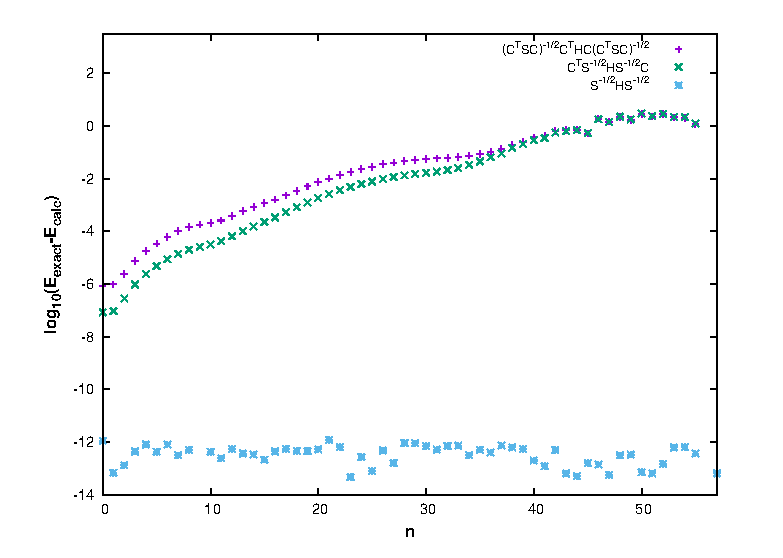
\includegraphics[width=6.5in]{./JCP2/fig1.eps}
\caption[Comparison of different symmetric chopping schemes for the harmonic oscillator]{Comparison of the accuracy of \Eq{halftogether} and \Eq{halfseparate} (or \Eq{standard}) for 
the harmonic oscillator Hamiltonian.  The starting basis of $800$ SG functions  is reduced to 
$56$ basis functions.  $n$ on the $x$ axis labels an  eigenvalue.  \label{Fig.ddhalfE}}
\end{figure}





 To use \Eq{halftogether}, which gives slightly better accuracy,   it is necessary to compute the retained corner of $ {\bf{    S^{-1/2}   H_G   S^{-1/2} }} $,
which  requires  summing over all 800 rows and  columns of    $ {\bf{  H_G   }} $.
In contrast,  to use  \Eq{standard}, one must only deal with $56 \times 56$ matrices.   For a multidimensional problem,  summing over all the SG functions in the 
original basis is not an option. However, for a multidimensional problem  $ {\bf{    S^{-1/2} }} $ can be computed and stored by exploiting its direct product
structure and if the PES is a SOP,  matrix-vector products can be evaluated without calculating the retained corner of $ {\bf{     S^{-1/2}   H_G   S^{-1/2}         }} $.   
%
Using Poirier's Weylet ideas,  it is possible to implement     \Eq{halftogether} without     summing over all the SG functions in the 
original basis. 





%
  In Figure \ref{Fig.ddoneE}   we compare \Eq{regulartogether}  and \Eq{standard}.  
  According to   \Refc{Brown2015b}, the eigenvalues of \Eq{regulartogether} should be significantly more 
  accurate than those of \Eq{standard}. 
  This is indeed the case.  
%
There are two reasons.   
First, in  \Eq{regulartogether}  800 columns of    ${\bf{     H_G     }} $ and 800 rows of  ${\bf{   S^{-1}          }} $  are retained.   
Second,   ${\bf{   (C^T S C)^{-1}          }} $ $ \ne {\bf{  C^T  ( S )^{-1}       C   }} $.
%
%




%JB added back X discussion
 The eigenvalues of \Eq{regulartogether}  are more accurate than those of  \Eq{halftogether} due to the fact that 
${\bf{    B   }} $ with elements  
 $B _{n,t} = \langle g_n \vert \psi_t \rangle $  has columns with small components and   the 
 corresponding elements of 
  ${\bf{   X = S^{-1/2}  B   }} $  are not as small.  They are not as small  because   the small components of   ${\bf{    B   }} $   get smeared out
 by  ${\bf{  S^{-1/2}       }} $.   This means that 
less error is introduced by chopping    ${\bf{     H_G  S^{-1}    }} $. 
We shall therefore use  \Eq{regulartogether}  for multidimensional calculations.   For multidimensional problems 
 $ {\bf{    S^{-1} }} $ will be  computed and stored by exploiting  direct product
structure.  For SOP PESs,  we  shall take advantage of direct product structure and not calculate  the  retained corner of $ {\bf{       H_G   S^{-1}         }} $.   



%
%
\begin{figure}[t]
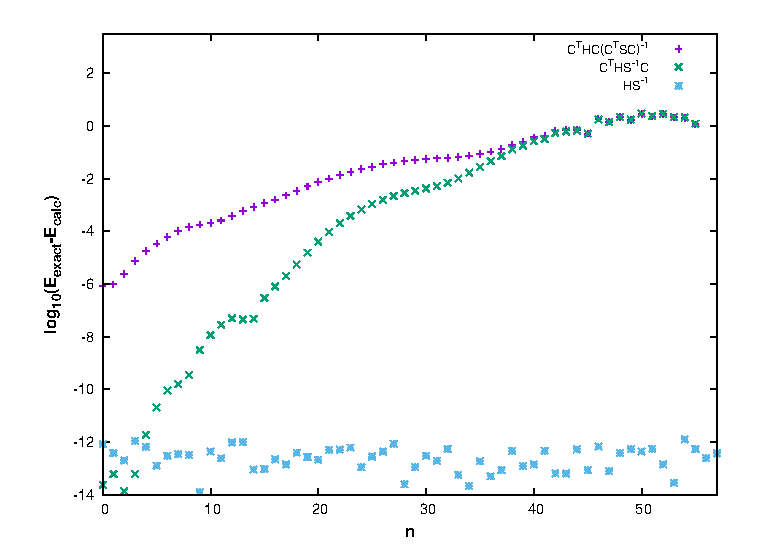
\includegraphics[width=6.5in]{./JCP2/fig2.eps}
\caption[Comparison of different asymmetric chopping schemes for the harmonic oscillator]{Comparison of  the accuracy of \Eq{regulartogether} and \Eq{regularseparate} (or \Eq{standard})  for the 
harmonic oscillator Hamiltonian.   A  starting basis with  $800$ SG functions is reduced to $56$ 
basis functions. $n$ on the $x$ axis labels an eigenvalue.    \label{Fig.ddoneE}}
\end{figure}





%

\section{Expanding a  basis of PSL functions\label{sec.expand}}

%


One wishes to choose a working basis 
that includes only the PSL functions corresponding to  large components of  the     columns of ${\bf{    B  }} $  associated with  desired energies.
It is not possible to solve the Schr\"{o}dinger equation in the full basis (with   $F $ functions).  Instead, one needs some 
means of determining which are the important functions.  
%
%
%  
%
 For the Hamiltonian,     

\begin{equation}
H=-\dfrac{1}{2}\dfrac{\mathrm{d}^2}{\mathrm{d}x^2}+\dfrac{1}{2}x^2+\dfrac{1}
{10}x^3+\dfrac{1}{100}x^4~,
\end{equation} 
% 
%
putting SG basis functions into  $\mathcal{R}_{E_{thres}} $  works less well.  



% 
%
Clearly,  it would be better to determine which PSL functions to include in the  working basis  by using  elements of   ${\bf{    B  }} $.    There are several schemes for expanding 
a PSL basis so that it includes the important functions.  \cite{Shimshovitz2014,Brown2015b}
%
\begin{figure}[t]
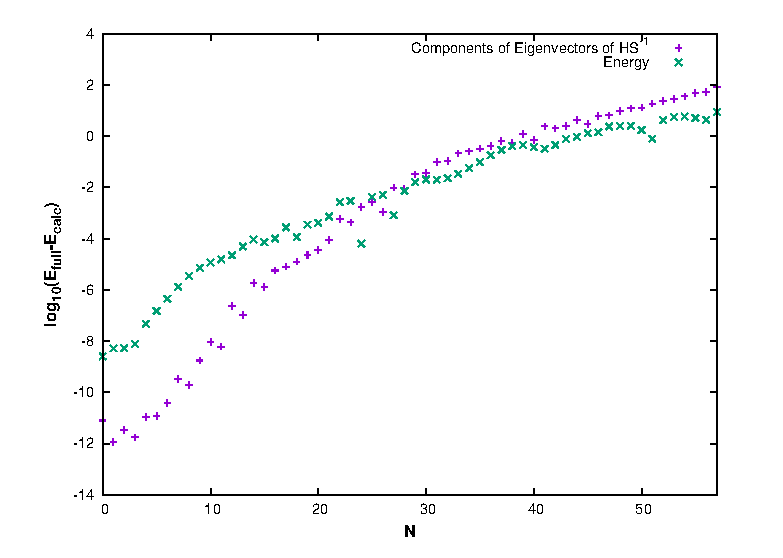
\includegraphics[width=6.5in]{./JCP2/fig3.eps}
\caption[Comparison of accuracy of classical energy and basis building scheme using phase-space localized basis functions.]{Comparison of the accuracy achieved by using a basis  composed of the 56 functions whose classical energy  is less than a threshold of 55,
%
and a basis 
composed of  the 56 functions for which components of eigenvectors of ${\bf{  H S^{-1}}}$  are largest        
 The latter basis is clearly better.\label{Fig.coefvE}}
\end{figure}
%
The scheme we use in this chapter begins by identifying 
a small set of  
 basis functions that are
 important and then adding new functions that are in some sense close 
to those deemed important.  
%
If  $\vert B_{nm}\vert$ is tiny then removing the $n$th basis function will have almost no effect on the    $m$th eigenvalue.   \cite{Brown2015b}  
It is also true that  if   $\vert B_{nm}\vert$  is large the  $n$th basis function is  important for calculating the    $m$th eigenvalue. 
We, therefore, deem a basis function important if 
$c^{sum}_n=\sum_{m=1}^{10} \left|  B_{nm}  \right|$ is large.     $c^{sum}_n$ is  the sum of the      
absolute values of  the components  of 
the 10 eigenvectors whose eigenvalues are smallest,   for a given basis function $n$. 
  %
%
If we retain the 56 basis functions with the largest values of $c^{sum}_n$,  we obtain a 
%
working basis 
with which the first 25 eigenvalues are 
 more accurate than those computed using  the 56 
functions that satisfy the $\mathcal{R}_{E_{thres}} $ criterion,  
  see Figure \ref{Fig.coefvE}. 
This establishes the advantage of using eigenvector components to determine which functions are 
included in the working basis  
%
to calculate the lowest energy eigenvalues.
For typical  spectroscopic problems, it is most important to calculate the lowest eigenvalues accurately.  However, if one wishes  to calculate a large number of eigenvalues 
to a fairly low accuracy level, a basis made with  the $\mathcal{R}_{E_{thres}}$ criterion might be better.  



  





%
%
For a real multi-dimensional problem, we want to build the working basis without knowing  ${\bf{   B}}$ and we therefore iteratively expand the basis  by 
successively adding to the  basis new functions, $d_{{\bf{n'}}}$,   
 whose phase-space centres are close to those of functions  $d_{{\bf{n}}}$  already in the basis and for which 
 $c^{sum}_{\bf{n}}$  is large.
For a multi-dimensional problem $  {\bf{n}} $ = $\{ n_1,n_2,   \cdots, n_D \} $.     
The  strategy is based on the  assumption  that  both wavefunctions and the basis functions  are  localized  and smooth
in phase space. 
%
%
To make the basis,  we first create a starting basis and then add functions to it.   Functions in the starting basis are those whose 
 phase-space centres are in a region      
 $\mathcal{R}_{E_{thres}} $  for a Hamiltonian that is the separable harmonic part of the full Hamiltonian and with a small $E_{thres}$.
%
The classical energy that corresponds to a PSL function is a sum of positive terms, one for each of the $2D$ 
terms in the   separable harmonic Hamiltonian.
To build the starting basis one must, in  principle, 
 consider for possible inclusion  all phase-space points in a huge direct product grid and for each of these points add up contributions 
from each of the $2D$ terms to obtain an energy, $E_{sum}$, and reject those functions for which   $E_{sum}  >  E_{thres} $.
%
 In practice,  for a given point, there is  no need to add 
contributions for all $2D$ terms because 
 when   $E_{sum}  >  E_{thres} $ there is no need to add contributions (all positive)  from other terms.   
%
There is also no need to loop over all points on the huge direct product grid.  
Assume the top loops are  over $n_{x_1}$ and $n_{p_1}$ and the bottom loops are over
 $n_{x_D}$ and $n_{p_D}$.  If, when considering for possible inclusion, 
  the         phase-space point $ n_{x_1},n_{p_1},   n_{x_2},n_{p_2},   \cdots   n_{x_D},n_{p_D} $,%
 after summing over terms  for $c=1,2,3$ ~  ,  
    $E_{sum} >  E_{thres} $,       
then there is no need to execute the remaining loops, for  $c=4,5, \cdots,  D$.
%
%
If nothing were 
 done to avoid looping over all the points of  the   huge direct product basis and all  the $2D$ terms,  the cost of determining which PSL to include in the starting basis would 
scale  exponentially with    $D$.     
 Halverson and Poirier\cite{Halverson2015} use    a more    
sophisticated method,  that defeats this exponential scaling,
to define their final basis which is defined so that it contains   all PSL functions with centres in 
 $\mathcal{R}_{E_{thres}} $,  for the full  Hamiltonian.  Determining only a starting basis is simpler.   







To generate the basis we do a set of Arnoldi calculations with increasing basis sizes.  The first Arnoldi calculation is done with the starting basis of the 
previous paragraph.      $c_{{\bf{n}}}^{sum}$ values are  calculated for each of  the $N_k$ functions in the starting basis.
  The   $c_{{\bf{n}}}^{sum}$     are then sorted using the Quicksort algorithm. \cite{Hoare1961}  
%
 We  add  to the basis neighbours of 
the PSL function with the largest  $c_{{\bf{n}}}^{sum}$, then neighbours of the PSL function with the 2nd largest  $c_{{\bf{n}}}^{sum}$, etc.  
When the size of the basis has been increased 5\% we stop adding functions.   
For a given ${\bf{n}}$, corresponding to   the phase space point $(n_{x_c}, n_{p_c})$, $c=1,2,...,D$, %
 the neighbours added  are  PSL functions  
with phase space points  $(n_{x_c}, n_{p_c})$, which are 
 1)    $n_{x_c}' = n_{x_c}$   and   $ n_{p_c}'$     
=  $n_{p_c}'+1$;
 2)    $n_{x_c}' = n_{x_c}-1$  and  $ n_{p_c}'$  =  $1$ ;
 3)   $n_{x_c}' = n_{x_c} +1$   and  $ n_{p_c}$  =  $1$.  
There are a total of $3 D$   neighbours.  
%
The basis composed of the starting basis and the    neighbours is the first expanded basis.  It  in turn is expanded to form the second expanded basis 
by doing another Arnoldi calculation and adding more neighbours.   The   process is repeated until we deem energy levels converged.   Each new basis is  
 5\% larger than the previous basis. 
%
We maintain a list of functions in the basis with index $m$,  and a list of $c_{{\bf{n}}}^{sum}$ values for functions in the basis for which we have not yet checked whether their neighbours should be included.  
%
   The $m$ corresponding to the largest $c_{{\bf{n}}}^{sum}$ values can be obtained from ${{\bf{n}}}$ using the mapping in the next section.      
  Before adding a neighbour, we use the same  mapping  to determine whether   it is  already in the basis.   
 %
The initial list  of $c_{{\bf{n}}}^{sum}$ values 
 includes   
all the  functions in the starting basis.     
% 
%
%
%
After adding     neighbours   for a particular basis function $\bs{n}$   to a  basis, 
we remove that     $c_{{\bf{n}}}^{sum}$   %
 from the list of  $c_{{\bf{n}}}^{sum}$   for    not-yet-checked functions. 
 $c_{{\bf{n}}}^{sum}$ is calculated only for functions in the not-yet-checked list.
%%
 This saves  computation time  in later  iterations due to the fact that many   PSL functions  have already had  their  phase-space neighbours added to the  basis. 
%  
%
%
It is perilous to determine  whether an eigenvalue is converged by comparing values at different basis sizes because the plot of an eigenvalue as a function of basis size 
may have plateaus.  
One way to ensure that eigenvalues are converged is to add basis functions until    the  $c_{\bs{n}}^{sum}$  of all the basis functions are all less than a small cutoff value.
  When  all $c_{\bs{n}}^{sum}$ in the not-yet-checked  list are below the  cutoff 
value, convergence is    achieved.
%
It might also be possible to use residuals to monitor convergence.  








\section{Computing a spectrum\label{sec.compit}}



Using the ideas of the previous sections, it is possible to sculpt a basis for a Hamiltonian.   Unfortunately, even the basis that includes only
the most important functions from a huge direct product basis is itself so large that most computers do not have enough memory to calculate eigenvalues of the 
basis representation of the Hamiltonian using methods of direct linear algebra.
Phase-space basis methods that require inverting an overlap matrix for the retained PSL functions are similarly limited by the need to store and manipulate large matrices.  \cite{Shimshovitz2014,Machnes2016} 
   One option is to use massively parallel computers.   \cite{Halverson2012,Halverson2014}    Another is 
to use an  iterative eigensolver.    
  Iterative eigensolvers  have been used to compute vibrational spectra for many years. \cite{Light2000,Bowman2008,Huang1999,Roy1995,Bramley1993,Mandelshtam1997,Iung1989,Yu1997,Chen1998} 
%
   They have the obvious advantage that they obviate the need
to store the Hamiltonian matrix.   Nevertheless, they are only efficient if there is a good way of evaluating matrix-vector products.    When the basis is a direct product,
 matrix-vector products can be efficiently evaluated by doing sums sequentially.\cite{Light2000,Bramley1993}   
%
  To use this idea, there is no need to build a Hamiltonian matrix because 
matrices representing 1D factors are sequentially  applied        to vectors.   These ideas cannot be used when the basis does not have product structure and a pruned basis 
built as explained in the previous section does not have product structure.    Avila and Carrington have shown that, despite pruning, it is possible to efficiently 
evaluate matrix-vector products by doing sums sequentially, {\it{ if basis functions are retained by imposing a pruning condition that itself has structure}}.\cite{Avila2009,Avila2011,Avila2015}
%
 A basis 
chosen to include only the important PSL functions will, in general, not have exploitable structure.    New ideas  are therefore required to evaluate matrix-vector products, in order to make iterative eigensolvers useful.


The technique we use to evaluate matrix-vector products only works if the Hamiltonian is a SOP.   Matrix-vector products are evaluated term by term and, for each term, factor by factor.  
We compute eigenvalues of $\bs{ H_G S}^{-1} $  where  $\bs{ H_G = \sum^t_{\ell} H_{\ell}  } $ and
${\bf{ S  = S_1 \otimes S_2 \otimes \cdots  S_D }}$.     To explain the ideas we shall focus on a single term,
  \be
{\bf{  H_{\ell}   = H^{\ell}_1 \otimes H^{\ell}_2 \otimes \cdots  H^{\ell}_D }} ~,  
\ee
 and therefore on    $\bs{ H_{\ell}}\bs{  S^{-1}}  =  \bs{H^{\ell}_1}\bs{ S_1^{-1}}  \otimes \bs{H^{\ell}_2  S_2^{-1}}   \otimes \cdots  \otimes  \bs{H^{\ell}_D S_D^{-1}}  = \bs{^1O^{\ell}}    \otimes  \bs{^2O^{\ell} }   \otimes    \cdots  \otimes \bs{ ^DO^{\ell} }   $.   
Note that many of the  
   ${\bf{  H^{\ell}_c}}, c=1,2, \cdots D$ factors may be (1D) overlap matrices.    
 If the PES is a Taylor Series then other  ${\bf{  H^{\ell}_c}}$   are  $\bs{x_c}^i, i=1,2,3,4$; others are  $\bs{  p_c}^2$
   We shall drop the superscript ${\ell}$ in the rest of this section.    
%
For one factor of one term,  the matrix-vector product one must evaluate could be written 
%
% 
\begin{equation}  
v_{n_{x_1}',n_{p_1}',...,n_{x_c}',n_{p_c}',..,n_{p_{D}}'}
= \sum_{n_{p_{c}}=1}^{N_{p_c}}
  \sum_{n_{x_c}=1}^{N_{x_c}}
%
      \bs{ ^cO}_{n_c^{\prime},n_c}
z_{n_{x_1}',n_{p_1}',...,n_{p_{c-1}}',n_{x_c},n_{p_c},n_{x_{c+1}}',n_{p_{c+1}}',..,n_{p_{D}}'} ~,
%
\label{jason-type}
\end{equation}
where $n_{x_c}$  and  $n_{p_c}$ are  position and momentum labels for coordinate $x_c$,  and   $n_c$  is a composite label that includes  
 $n_{x_c}$  and  $n_{p_{c}}$.   $ \bs{ ^cO}_{n_c^{\prime},n_c}$ depends on  $n_{x_c}$  and  $n_{p_{c}}$  and  $n'_{x_c}$  and  $n'_{p_{c}}$   because each 1D basis function has  both 
 position and momentum labels.   
%
  The vectors are stored in a 1D array indexed by $m$ and the matrix-vector product      is
  \begin{equation}
  \begin{split}  
v(m'(n_{x_1}',n_{p_1}',...&,n_{x_c}',n_{p_c}',..,n_{p_{D}}'))
= \\ &\sum_{np_{c}=1}^{Np}
  \sum_{nx_c=1}^{Nx}
%
      \bs{ ^cO}_{n_c^{\prime},n_c}
z(m(n_{x_1}',n_{p_1}',.. ,n_{p_{c-1}}'  ,n_{x_c},n_{p_c},  n_{x_{c+1}}',..,n_{p_{D}}')) ~,
%
\end{split}
\label{eq.sopmv}
\end{equation}
The sums must be done for  $m'$ =$ 1, 2, \cdots,  N_k$.
 Knowing a value of $m'$ one finds values of ${n_{x_1}',n_{p_1}',...,,n_{x_c}',n_{p_c}',...,n_{p_{D}}'}
$ from a $N_k \times 2D$ table that is stored.   The table is denoted $A$.  Its 
$m'$th row contains   the $2D$ ${n_{x_1}',n_{p_1}',...,n_{x_c}',n_{p_c}',...,n_{p_{D}}'}
$   labels  for the  $m'$th      basis function. 
%
Note that we are not, as is often the case when 
evaluating matrix-vector products in a pruned basis, 
transforming the input vector into the output vector, index by index sequentially, with  $D+1$  nested loops.
%
   When indices are transformed sequentially, the 
transformed and untransformed indices are separately constrained.  In this case, the length of intermediate vectors increases and then 
decreases.   \cite{Avila2009,Wang2001c}    
% 
Instead, for each factor, the vector on the LHS of \Eq{eq.sopmv} has only as many elements as there are retained basis functions.  
This is similar to the strategy of \Refc{Cooper2009}.
%JB should this go above? "Note that we are not..."
 





It remains to explain how knowing  $
{n_{x_1}',n_{p_1}',...,  n_{x_{c-1}}',n_{p_{c-1}}',n_{x_c},n_{p_c},n_{x_{c+1}}',n_{p_{c+1}}'...,n_{p_{D}}'}$ one finds $m$, which labels the input vector.    In principle this could be done 
by storing a 
 $D$ 
dimensional array  with  $(N_xN_p)^{D}$ elements,  whose value is  $m$, if the corresponding function is in the basis, 
and  0, if the corresponding function is not in the basis.   
Of course, this is impossible because the array is huge.  It is also not necessary because many of the elements of the array would be zero.   
Instead, we use a recursive mapping.   It is determined by making a list of retained 
 $
{n_{x_1},n_{p_1},...,,n_{x_c},n_{p_c},...,n_{p_{D}}}$ functions and labelling them with $m=1,2,  \cdots N_k$.
 It works regardless of the order of the retained basis functions. 
%
%
 The idea is illustrated by giving here an example with two coordinates and four indices $
{n_{x_1},n_{p_1},n_{x_2},n_{p_2}}$ which for simplicity will be written ${t_1,t_2,t_3,t_4}$.  
%
If there are four indices, we store four matrices,
 ${\bf{T_1,T_2,T_3,T_4}}$ which are 
initialized as zero matrices.    
Non-zero elements of  ${\bf{T_1,T_2,T_3,T_4}}$ are determined as follows.  
The smallest value of $m$ for  which  $t_1 = k_1$  (regardless of $t_2,t_3,t_4$)    is denoted  $m_{k_1}$ and is stored in   $T_1(1,k_1)$.   The subscript on $T$ indicates
that it is for   $t_1$.   
The smallest value of  $m$ for  which  $t_1 = k_1$  and 
 $t_2 = k_2$ (regardless of $t_3,t_4$)
is  labelled as $m_{k_1,k_2}$      and  stored in $T_2(m_{k_1},k_2)$. 
The smallest value of  $m$ for  which  $t_1 = k_1$,  $t_2 = k_2$  and  $t_3 = k_3$   (regardless of $t_4$)
is labelled as $m_{k_1,k_2,k_3}$   and   stored in $T_3(m_{k_1,k_2},k_3)$.    
The  value of  $m$ for  which  $t_1 = k_1$,  $t_2 = k_2$,  $t_3 = k_3$, and   $t_4 = k_4$
is  labelled as $m_{k_1,k_2,k_3,k_4}$ and is stored  in  
 $T_4(m_{k_1,k_2,k_3},k_4)$.  This mapping can be extended to many more dimensions by simply adding more ${\bf{T_i}}$ matrices.

% 
%
%
The memory cost of this mapping is relatively low.  Assuming that we use the same  
${N_x}$ and 
$ {N_p} $ for all coordinates,   the   ${\bf{T}}$  matrix     for a coordinate index  has 
$(N_k+1) N_x$ elements and the  ${\bf{T}}$  matrix     for a momentum index  has 
$(N_k+1) N_p$ elements.  
%
%
Each  ${\bf{T}}$  matrix  has      $N_k+1$ and not   $N_k$  rows  because this reduces the number of 
if statements required.   We add a zeroth row with elements    $T_c\left(0,k_c\right)$=0.    
so that  
%
when  $  m_{k_1,...k_{c-1}}$   = $    T_{c-1}\left(m_{k_1,...k_{c-2}},k_{c-1}\right)=0$, i.e.  the    basis function with labels $k_1,...,k_{c-1},k_c$ is not in the retained basis,
%
 $T_c\left(m_{k_1,...k_{c-1}},k_c\right)=T\left(0,k_c\right)=0$ and does not need to be set to zero by using if statements.   
%
 Only one if statement, after all $D$ $T_c$ matrices have been used, is necessary to determine if a basis function is in the retained basis. Namely, if $m_{k_1,...,k_D}=0$ then the basis function with indices $k_1,...k_D$ is not in the retained basis.  
%
%
 The total memory cost is therefore $(N_k+1)  D  (N_x+N_p)$.   If $N_x$ and $N_p$ were  different for different coordinates, it would be 
$  (N_k + 1) \sum_c  (N_{x_c}+N_{p_c})$.
% 
%










%
We actually do not sum over $n_{x_c}$,  as indicated in \Eq{eq.sopmv}.   For a set of labels on the output vector, i.e.,   $
{n_{x_1}',n_{p_1}',...,,n_{x_c}',n_{p_c}', ,   ...,n_{p_{D}}'}$, which corresponds  to $m'$, we need to sum 
not over \emph{all}  $n_{x_c}$ values, but only over  all  possible $n_{x_c}$ values.  This is done by 
using another mapping.   The matrix-vector product is,
\begin{equation}
\begin{split}
v(m'(n_{x_1}',n_{p_1}',..&., n_{x_c}',n_{p_c}',...,n_{p_{D}}'))
= \\
 &\sum_{l_{x_c}=1}^{U_{x_c}({m'})}
  \sum_{n_{p_c}=1}^{U_{p_c}({m''})}
%
      \bs{ ^cO}_{n_c^{\prime},n_c}
z(m({n_{x_1}',n_{p_1}',...,n_{p_{c-1}}',n_{x_c},n_{p_c}, n_{x_{c+1}}',   ...,n_{p_{D}}'})) ~,
%
\end{split}
\label{with_nm}
\end{equation}
%
  The reason we sum over $l_{x_c}$, rather than 
 $n_{x_c}$,  is that 
basis functions with $2D-2$ indices 
$n_{x_1}',n_{p_1}',..., n_{p_{c-1}}',n_{x_{c+1}}',...,n_{p_{D}}'$
do not exist for    some   $n_{x_c}$.   If we sum over  $l_{x_c}$, we 
can sum over consecutive values.    
%
Due to the method used to add basis function neighbours in Section \ref{sec.expand}, there are no holes in the $n_{p_c}$ index list  
 and therefore no need for an $l_{p_c}$ index.  For any $n_{x_c}$; $n_{p_c}=1$ is always added first; $n_{p_c}=2$ is always added second; etc. 
%
To use \Eq{with_nm} one must find $n_{x_c}$  from $l_{x_c}$.  
% 

%
%
%

%
We  make two matrices,   ${\bf{M_{x_c}}}$ and ${\bf{M_{p_c}}}$, defined so that a row contains 
 position indices   of basis functions  that have  indices  
$n_{x_1}',n_{p_1}',..., n_{p_{c-1}}',n_{x_{c+1}}',...,n_{p_{D}}'$. 
%
%
 From the position index stored in  ${\bf{M_{p_c}}}$, we find   
 $n_{x_{c}}$ using Table $A$.   
%
In \Eq{with_nm},  
$ U_{x_c}(m')$, $ m'=1, \cdots,  N_k$,  is  the number of different 
 $n_{x_{c}}$ values that occur in the basis, for  particular values of  $n_{x_1}',n_{p_1}',..., n_{p_{c-1}}',n_{x_{c+1}}',...,n_{p_{D}}'$, regardless of the value of    $n_{p_{c}}$.
% 
The functions with the smallest  $n_{x_{c}}$ are labelled by  $l_{x_{c}}=1$; 
the functions with the  second smallest  $n_{x_{c}}$ are  labelled by  $l_{x_{c}}=2$; etc.  
%
 $M_{x_c}(m',l_{x_c})$  is     the 
position,     denoted  $m''$,      in $A$ of the basis function      with  $l_{x_c}$,    $n_{p_c}=1$  and 
 $({n_{x_1}',n_{p_1}',...,n_{p_c{-1}}',n_{x_{c+1}}',...,n_{p_{D}}'})$.  
$m'$  labels the component of the output vector being computed.   $n_{p_c}=1$ is used because the basis function with  $n_{p_c}=1$ is always retained.  
%
$M_{x_c}(m',l_{x_c})$ is stored as a $N_k\times N_{x_c}$ matrix. 
%
%
% 
%
  $U_{p_c}(m'')$ is  the number of $n_{p_c}$ values for a given set of $2D-1$ indices,  
  $({n_{x_1}',n_{p_1}',...,n_{p_c{-1}}',n_{x_{c}},n_{x_{c+1}}',...,n_{p_{D}}'})$.
  $U_{p_c}(m'')$ is a vector of length $N_k$.  
%
 ${\bf{M_{p_c}}}$ is stored as a  $N_k\times N_{p_c}$ matrix  and 
$M_{p_c}(m'',n_{p_c}) = p$   is the position  in $A$ of the basis function      with  $l_{x_c}$,    $n_{p_c}$  and 
$({n_{x_1}',n_{p_1}',...,n_{p_c{-1}}',n_{p_{c+1}}',...,n_{p_{D}}'})$.   From the position, 
$n_{x_c}$ can be obtained from the $m${th} row of table $A$.







An example should make this easier to follow.    A    2D problem with $6$ basis functions  has the  $A = A_e$ table shown in 
 Table \ref{Tab.A}.
\begin{table}
\centering
\begin{small}
\caption{\label{Tab.A} An example retained basis set table $A_e$ of indices.}
\begin{tabular}{|c | c   c  c  c |  }
\hline
m & $n_{x_1}$ & $n_{p_1}$ & $n_{x_2}$ & $n_{p_2}$ \\	
\hline
 1 & 2 & 1 & 2 & 1 \\       
 2 & 1 & 1 & 2 & 2 \\
 3 & 1 & 1 & 2 & 1 \\
 4 & 1 & 1 & 4 & 1  \\
 5 & 1 & 1 & 4 & 2 \\
 6 & 1 & 1 & 2 & 3  \\          
  \hline                
\end{tabular} 
\end{small}
\end{table} 
%
If  $c=2$, so that the sum is over $l_{x_2}$ and $p_{x_2}$,   and we are computing   the component     $m'=6$ with indices  $(n_{x_1},n_{p_1},n_{x_2},n_{p_2})=(1,1,2,3)$, 
then $U_{x_2}(6) = 2$  and the two   possible $n_{x_2}$ values are  $2,4$ ($n_{x_1}=n_{p_1}=1$).    
%
 $l_{x_2}=1$ corresponds  to $n_{x_2}=2$ and   $l_{x_2}=2$ corresponds  to $n_{x_2}=4$.  
 %
With  $l_{x_2}=1$ (or $n_{x_2}=2$ ) and $n_{p_2}=1$,  the position in $A_e$    is 3 so 
 $m''=M_{x_2}(6,1)=3$. This is the basis function with  indices $(1,1,2,1)$.    
%
  $U_{p_2}(3)=3$  because there are three    possible $n_{p_2}$ values:   $1,2,3$.
The rightmost  sum in  \Eq{with_nm} is  therefore over 
 $n_{p_2}=1,2,3$. 
The corresponding  $m$ positions in $z$ contributing to the sum are 
 $M_{p_2}(3,1)=3,M_{p_2}(3,2)=2,M_{p_2}(3,3)=6$.    
%
%
With $l_{x_2}=2$ ( $n_{x_2}=4$),    $M_{x_2}(6,2)=4$,   
  and $U_{p_2}(4)=2$  because there are two 
possible values of  $n_{p_2}$ (they are 1 and 2).   The $m$ values to be summed are therefore  $M_{p_2}(4,1)=4,M_{x_2}(4,2)=5$.  
Note that the double sum corresponds to adding contributions from $m$ in the order $3,2,6,4,5$.  
As is necessary, position $m=1$ of $z$ does  not contribute.

%















\section{Test calculations: P$_2$O, CH$_2$O, CH$_2$NH  }   
We  use  the ideas of sections \ref{2sec2}, \ref{Sec.chop} , \ref{sec.expand},  and \ref{sec.compit}     
to compute vibrational energy levels of three realistic (but SOP) Hamiltonians:   a 
 P$_2$O Hamiltonian  (with the PES    of Pouchan \emph{et al}\cite{Pouchan2001}), a CH$_2$O  Hamiltonian   (using a refitted 
potential  based on  \Refc{Martin1993}),
%
 and  a  CH$_2$NH    Hamiltonian    (using the potential of 
Pouchan and Zaki\cite{Pouchan1997}, as interpreted in \Refc{Halverson2014}).  These calculations enable us  to test the efficiency of the method.
Testing with    molecules having  three, four, and five atoms, 
we shall  show how the method scales in practice,  when spectroscopic accuracy is 
required.  



We present only results with the SG PSL basis of Halverson and Poirier (HP).    
Although we use the same SG basis as HP,  our calculations differ from theirs.    1) We compute eigenvalues of the product   ${\bf{H_G S^{-1}}}$; the number of
columns of  ${\bf{H_G }}$ (and the number of rows of  ${\bf{ S^{-1}}}$) is larger than the number of rows of  ${\bf{H_G }}$ (and the number of columns of  ${\bf{ S^{-1}}}$).
2)   We use a different approach to selecting SG PSL functions to retain.
3) To make it possible to retain a huge number of    SG PSL functions, we use an iterative eigensolver.   
%
We do not report results obtained with a Gaussian basis.   The SG results are systematically better because   
the SG  functions have phase-space boxes that are 
smaller, with size (in 1D)  $h/2$,   than the Gaussian phase space boxes which (in 1D) have size    $h$. 
As explained by HP,  smaller phase space boxes  enables one to cover the important region of phase space with less waste.
All matrix elements are calculated exactly.   
The SG basis  could also be used to contract a direct product DVR, as was done previously with a Gaussian basis.
\cite{Shimshovitz2012,Brown2015,Brown2015b,Shimshovitz2012,Shimshovitz2014}
Using the DVR obviates the need to use a SOP PES, but for a SOP PES there is no reason not to use the SG  basis directly.   
With a Gaussian basis, it is better to use it to contract a DVR because without a DVR  the number of  
  columns of  ${\bf{H_G }}$ (and the number of rows of  ${\bf{ S^{-1}}}$) required to get converged eigenvalues is huge.   











\subsection{Choosing the 1D basis sets}


%

We need to specify  exterior and  interior  1D bases, i.e. choose $f^i$ and $f^e$ 
(see \Eq{op}).
  There are $\mathcal{N}_e$  1D exterior basis functions;  $\mathcal{N}_e = \mathcal{N}_x^e  \mathcal{N}_p^e$, where  $\mathcal{N}_x^e$ is the number of
exterior position labels and  $  \mathcal{N}_p^e$ is the number of exterior momentum labels.
 There are $\mathcal{N}_i$  1D interior basis functions;  $\mathcal{N}_i = \mathcal{N}_x^i  N_p^i$, where  $\mathcal{N}_x^i$ is the number of
interior  position labels and  $  \mathcal{N}_p^i$ is the number of interior  momentum labels.     
 Products of the  1D basis functions are  the multi-dimensional basis functions.
%
 $\mathcal{N}_e^D$ is the number of rows of ${\bf{H_G}}$  (and columns of    ${\bf{S^{-1}}}$)  in \Eq{regulartogether}.    
 $\mathcal{N}_i^D$ is  the number of columns  of ${\bf{H_G}}$  (and rows of    ${\bf{S^{-1}}}$  in \Eq{regulartogether}.    
We choose  a large  $\mathcal{N}_i$.   This does not significantly increase the cost of the calculation   because 
 ${\bf{H_G}}$ is a sum of direct products   and    ${\bf{S}  }$  is also a  direct product.     The size of   ${\bf{S^{-1}}}$  is
 $\mathcal{N}_i^D \times  \mathcal{N}_i^D$, but we only invert  $\mathcal{N}_i \times  \mathcal{N}_i$ matrices.
%
To ensure accurate levels we take  
 $\mathcal{N}_x^i=40,\mathcal{N}_p^i=20$ which corresponds to a  grid of points at 
$(\sqrt{\pi}(n_x-20)-\sqrt{\pi}/2,   \sqrt{\pi}(n_p-1)+\sqrt{\pi}/2)$  
where 
$n_x=1, \cdots ,40,n_p=1, \cdots, 20$.       
This may be larger than necessary.  
We choose       $\mathcal{N}_x^e$ = 12 and $\mathcal{N}_p^e$ = 6.      This  
 corresponds to grid points at $(\sqrt{\pi}
(n_x-6)-\sqrt{\pi}/2,     \sqrt{\pi}(n_p-1)+\sqrt{\pi}/2)$ where $n_x=1, \dots, 12,n_p=1, \cdots ,6$.  
These values are chosen because 
$\mathcal{N}_i=12,\mathcal{N}_j=6$ is the smallest  direct product (in phase-space) basis with which  one can 
calculate the lowest 6 energy levels of  the Harmonic oscillator to machine 
precision.    With this 1D basis, we are certain 
 that it is possible to calculate  accurate  levels of the multi-dimensional Hamiltonians, if enough multi-dimensional basis functions 
are retained.    We choose   $\mathcal{N}_e  < \mathcal{N}_i$ because decreasing   $\mathcal{N}_e$ reduces the size of the $M$ and $T$ mappings and 
decreases the size of all the ${\bf{ ^cO}}$ matrices.   
%
The maximum  indices $N_{x_c},N_{p_c}$ are equal for all $c$ in our calculations,  and 
 $N_{x_c}=\mathcal{N}_x^e=12$ and $N_{p_c}=\mathcal{N}_x^e=6$.
  %


Before launching the iterative eigensolver we compute a set of $72 \times 800$ matrices.   The same 1D basis is used for all coordinates and we
therefore only need to compute   
%
matrices for  $x_1,x_1^2,x_1^3,x_1^4,-\dfrac{\partial^2}{\partial x_1^2}$.   
%
We also need  a  $800  \times 72$ matrix 
 ${\bf{ S^{-1}_1}}$ (the same for all coordinates).  It is obtained from elements of the inverse of the 
$800 \times  800$  matrix $\bs{S_1}$.   
%
%










\subsection{Results}

%
ARPACK with the reverse communication driver dnaupd is used to perform all calculations.  The 
number of columns (NCV) is taken to be three times the size of the number of eigenvalues (NEV) 
calculated,  for each molecule studied. The default stopping criteria of machine precision is 
used for the calculations.\cite{Lehoucq1998b} Although RULE \cite{Tremblay2007} could also be used, ARPACK is more robust.    
  
  
 Levels of    P$_2$O  are reported in columns 4 and 5 of    Table   
\ref{Tab.1}. The levels published by HP %
(columns 2 and 3) 
are about as accurate as those we compute with both having an error of less than $0.1$cm$^{-1}$.  \cite{Halverson2014} 
%
  However, we  attain similar accuracy with  a PSL basis whose size is two orders of magnitude smaller.   
%
Our basis is much smaller because we do not chop the 
 ${\bf {S }}$ and  ${\bf{ H_G }}$  matrices separately (we use \Eq{regulartogether} and \Eq{halftogether})
 and because we use a different procedure for determining which basis functions to retain.    
It is our basis function selection method (section \ref{sec.expand})     that is the most important.   
Using our basis selection method, but  chopping  ${\bf{ S }}$ and  ${\bf{ H_G }}$  separately (i.e. \Eq{standard}), rather than using \Eq{regulartogether}   increases  the size of the SG basis required to obtain  levels   within  $0.1$cm$^{-1}$ of  numerically exact levels,      
by more than a factor of two.   
%
The eigenvalues of  \Eq{halftogether}    %in the table 
 are close to those of  \Eq{standard}  % w wc i vgl in previous sentence 
because the 
 eigenvalues  of  \Eq{halftogether} are close to those of   \Eq{halfseparate} (see section \ref{sec.expand})  and the eigenvalues of   \Eq{standard}) are equal to those of 
 \Eq{halfseparate}.   
%
  The advantage of \Eq{regulartogether} is therefore significant, but much less important than the advantage of the new 
basis function selection procedure.     


Although with   \Eq{halftogether} one   requires  requires a larger basis to achieve the same accuracy      (compare columns 4 and 5), 
\Eq{halftogether}  has the significant advantage that it is a 
 symmetric eigenproblem and  therefore the Lanczos algorithm can be applied.  Owing to the fact that the memory cost of the 
 Lanczos algorithm is much less (only two vectors of length $N_k$ must be stored)    than that of ARPACK  (which requires many vectors),
 \Eq{halftogether} could be used with a much larger basis.  
% 
%
%
%
%
When using  Lanczos, the $c_m^{sum}$ values would   be calculated from eigenvectors computed   by doing  
a second set of Lanczos iterations,  \cite{Bramley1994b,Wang2003b}
 with no additional memory requirements.  Implemented in this fashion,   
 the   memory cost is dominated by    the mappings.  
 %
There would also be additional computation required to force the Hamiltonian matrix  to be Hermitian.\cite{Cooper2009} 
%
%


%
 It is encouraging that it is possible to 
significantly decrease the size of the SG basis. 
%
  However, even our SG basis is much larger than  the    HOB basis built using 
 \Eq{Eq.HOBprune} with $N=17$,   
which is  good enough to converge all the levels in the table to  three decimal places,        
%
It is surely possible to reduce the size of the HOB further by using a   better  pruning condition. $  \sum_c g_c(x_c) \le N$ with carefully chosen $g_c(x_c)$ would be much 
better.  Even 
$\alpha_1 n_1 +  \alpha_2 n_2 +  \alpha_3 n_3 $ with $\alpha_c \ne 1$ would be better.  Even with   $ n_1 +  n_2 +  n_3 \le N  $,  the HOB is about an order of magnitude 
smaller than our best SG basis (and three orders of magnitude smaller than the HP SG basis).
%



%
%
\begin{table}
\centering
\begin{small}    
\caption[The lowest 26   vibrational   
levels of   P$_2$O]{\label{Tab.1} The lowest 26   vibrational   
levels (with respect  to the zero point energy)  of   P$_2$O. 
%
}
\begin{tabular}{|l | r | r | r | r | r| }
\hline
State& \multicolumn{2} {|c|}{\Refc{Halverson2014}}  & \multicolumn{1} {|c|}
{\Eq{regulartogether}} & \multicolumn{1} {|c|}{\Eq{halftogether}} & \multicolumn{1} {|c|}
{HOB}\\	
\hline
Basis size & \multicolumn{1} {|c|}{201414}  & \multicolumn{1} {|c|}{405521}  & 
\multicolumn{1} {|c|}{$4995$} & \multicolumn{1} {|c|}{$11033$} & \multicolumn{1} 
{|c|}{1140}\\	
	\hline                
 $v_1$             &    197.481    &    197.474    &     197.479    &   197.481 & 197.479\\                   
 2$v_1$            &    395.464    &    395.452    &     395.461    &   395.465 & 395.463\\                   
 3$v_1$            &    593.930    &    593.914    &     593.928    &   593.935 & 593.929\\                   
 $v_2$             &    643.912    &    643.968    &     643.900    &   643.900 & 643.897\\                   
 4$v_1$            &    792.858    &    792.838    &     792.858    &   792.867 & 792.858\\                   
 $v_1$ + $v_2$   &    839.844    &    839.893    &     839.827    &   839.832 & 839.826\\                   
 5$v_1$            &    992.228    &    992.205    &     992.227    &   992.241 & 992.228\\                   
 2$v_1$ + $v_2$  &   1036.272    &   1036.316    &    1036.251    &  1036.261 &1036.252\\                   
 6$v$1             &   1192.018    &   1191.991    &    1192.022    &  1192.037 &1192.018\\                   
 3$v_1$ + $v_2$  &   1233.174    &   1233.213    &    1233.158    &  1233.170 &1233.154\\                   
 $v_3$             &   1265.393    &   1265.411    &    1265.308    &  1265.308 &1265.295\\                   
 2$v_2$            &   1290.641    &   1290.537    &    1290.610    &  1290.623 &1290.599\\                   
 7$v_1$            &   1392.207    &   1392.176    &    1392.221    &  1392.236 &1392.206\\                   
 4$v_1$ + $v_2$  &   1430.530    &   1430.563    &    1430.515    &  1430.529 &1430.509\\                   
 $v_1$ + $v_3$   &   1460.187    &   1460.196    &    1460.092    &  1460.100 &1460.082\\                   
 $v_1$ + 2$v_2$  &   1485.176    &   1485.071    &    1485.141    &  1485.170 &1485.134\\                   
 8$v_1$            &   1592.771    &   1592.738    &    1592.787    &  1592.813 &1592.770\\                   
 5$v_1$ + $v_2$  &   1628.317    &   1628.344    &    1628.296    &  1628.319 &1628.294\\                   
 2$v_1$ + $v_3$  &   1655.502    &   1655.507    &    1655.402    &  1655.419 &1655.396\\                   
 2$v_1$ + 2$v_2$ &   1680.214    &   1680.110    &    1680.180    &  1680.220 &1680.172\\                   
 9$v_1$            &   1793.689    &   1793.652    &    1793.704    &  1793.745 &1793.687\\                   
 6$v_1$ + $v_2$  &   1826.512    &   1826.532    &    1826.507    &  1826.524 &1826.488\\                   
 3$v_1$ + $v_3$  &   1851.319    &   1851.321    &    1851.237    &  1851.249 &1851.213\\                   
 3$v_1$ + 2$v_2$ &   1875.735    &   1875.631    &    1875.719    &  1875.769 &1875.692\\                   
 $v_2$ + $v_3$   &   1897.546    &   1897.512    &    1897.449    &  1897.447 &1897.421\\                   
 3$v_2$            &   1936.341    &   1936.288    &    1936.284    &  1936.299 &1936.260\\                   
    \hline                
\end{tabular} 
\end{small}
\end{table}







Of course, it is important to test \Eq{regulartogether} on a problem with a larger $D$.    We therefore also did calculations on  CH$_2$O.   This 
enables us to examine how the cost of the  method scales with  basis size.
%
We first did calculations on the PES of   Romanowski et al.\cite{Romanowski1985}   
Although the   Romanowski  PES is  usable with a pruned  harmonic oscillator basis,  it has holes 
(i.e. spurious minima)
that 
make it  impossible to converge energy levels using SG functions.  
%
Instead,  we used a PES    obtained from the PES of \Refc{Martin1993}  by
calculating derivatives with respect to normal coordinates to make a Taylor series approximation. \cite{gab}
%
Many energy levels converged with the  Taylor series  PES.   
%
 The lowest 
thirty energy levels, computed with the same methods as for P$_2$O,  are shown in Table \ref{Tab.2}. 
%
These levels are low enough that they are probably not shifted by holes in the PES.
%
For  CH$_2$O, the HOB,  pruned with    $ n_1 +  n_2 +  n_3 +n_4 +n_5 + n_6 \leq 15  $,
%
 which is large enough to converge all the energies in the table to the number of digits shown, 
is about 14 times   smaller  than the best SG basis.   
To some extent the size of the  SG basis is inflated by the holes   
still present in the re-fitted PES.  
This is due to the fact that our basis function selection algorithm  
 has a propensity to add SG functions    in    holes.   However, even    if these  SG functions are removed from the basis,  the SG basis is still about  an order of magnitude 
larger than the HOB basis. 
%
%





\begin{table}
\centering
\begin{small}
\caption[The  lowest 30 calculated vibrational energies of CH$_2$O]{\label{Tab.2} The  lowest 30 calculated vibrational energies of CH$_2$O.
%
 Levels computed with \Eq{regulartogether} are   compared to
those computed with  a pruned harmonic basis.     
 }
\begin{tabular}{|l | r | r | }
\hline
State&\multicolumn{1} {|c|}{\Eq{regulartogether}}  & \multicolumn{1} {|c|}{HOB}\\	
\hline
Basis size & \multicolumn{1} {|c|}{$713883$} & \multicolumn{1} {|c|}{$54264$}\\	
	\hline                
  1    &  5781.022 & 5781.019\\                   
  2    &  6937.357 & 6937.344\\                   
  3    &  7030.013 & 7030.001\\                   
  4    &  7283.862 & 7283.837\\                   
  5    &  7530.419 & 7530.383\\                   
  6    &  8088.318 & 8088.248\\                   
  7    &  8196.896 & 8196.848\\                   
  8    &  8274.013 & 8273.950\\                   
  9    &  8437.703 & 8437.642\\                   
 10    &  8503.379 & 8503.319\\                   
 11    &  8569.769 & 8569.707\\                   
 12    &  8617.996 & 8617.937\\                   
 13    &  8677.273 & 8677.166\\                   
 14    &  8781.941 & 8781.841\\                   
 15    &  8784.038 & 8783.958\\                   
 16    &  9025.296 & 9025.137\\                   
 17    &  9226.167 & 9225.849\\                   
 18    &  9262.918 & 9262.840\\                   
 19    &  9355.044 & 9354.847\\                   
 20    &  9448.225 & 9448.042\\                   
 21    &  9507.199 & 9506.904\\                   
 22    &  9583.644 & 9583.429\\                   
 23    &  9637.372 & 9637.242\\                   
 24    &  9696.828 & 9696.623\\                   
 25    &  9701.028 & 9700.894\\                   
 26    &  9744.542 & 9744.372\\
 27    &  9791.924 & 9791.786\\                   
 28    &  9817.159 & 9816.758\\                   
 29    &  9854.375 & 9854.175\\                   
 30    &  9934.984 & 9934.785\\
    \hline                
\end{tabular} 
\end{small}
\end{table}




To further test \Eq{regulartogether} and assess the utility of PSL bases, we have also computed energy levels of  CH$_2$NH, for which $D=9$.  In this case, 
a direct product harmonic basis is large enough that the memory cost of a simple direct product Lanczos calculation is prohibitive.   It is for such 
problems that one needs new ideas.  
We use the  potential of   \Refc{Pouchan1997},  as interpreted by HP in        \Refc{Halverson2014}.    The sums over indices are constrained and there are factorial terms in 
front of the sums.   
  \cite{Halverson2014}.  In  \Refc{Halverson2014}, HP use their SG basis to compute vibrational levels.   
Our results are summarized  in  Table \ref{Tab.3}. 
%
We see no evidence that our basis functions are sampling holes. 
 To converge the first 10 levels to within about 1  cm$^{-1}$ we require about $26 \times 10^6$ SG functions.  
%
It is impossible to compare our results with those of HP for two reasons:  1)   their convergence errors  are  much larger than  1  cm$^{-1}$; 2) two of the their force constants
are not the values reported in the table of     \Refc{Pouchan1997}.\cite{Halverson_priv}   
%
%
Energy levels computed with the largest basis in  \Refc{Halverson2014}  are reported in column 4.    
These energies were generously provided by the authors.   
%
% 
Our best SG basis, with which one $can$ compute accurate levels,  is  more than two orders of magnitude 
larger than the very simple HOB basis built  from the pruning condition $\sum_c n_c \le N$.  Much better HOB bases could be devised.  
It appears that if  one wishes accurate levels, the SG basis, which is the best known PSL basis, is not competitive for molecules like   CH$_2$NH and 
 CH$_2$O.   


 It might be true, that if one  were satisfied with less accurate levels and needed  more of them that the SG basis would be competitive.   However, the 
levels reported in \Refc{Halverson2014}  have large convergence errors.  
%
The two largest bases used by HP have 212197  and 409581 functions.   It is dangerous to assume that the difference between energies computed with two SG bases  is a good
measure of convergence error.     \cite{Halverson2012,Halverson2014,Halverson2015}  
One might conclude from    Table  IV  of \Refc{Halverson2014},  that  the convergence error  of  the   first $ frequency$   (i.e. difference between the first level and the zpe(zero point energy)) is about 
5  cm$^{-1}$.   Reported energy level differences   for the first 10 frequencies  are all less than about 43  cm$^{-1}$.   
According to Table  V  of \Refc{Halverson2014}, there are 11 states for which the difference between levels computed with the two  largest HP bases is less than 1  
cm$^{-1}$.   
%
HP underestimate their convergence error.   With  409'581 
functions their  lowest frequency is 
1212.581  cm$^{-1}$.  
%
     The converged value (on their PES) is  1105.56cm$^{-1}$, see column 5 of Table   \ref{Tab.3}.       Therefore, the true  error is not   about   5 but  about 100cm$^{-1}$.
Errors in the first 10 levels (not frequencies) are about 
 1000cm$^{-1}$; see Table \ref{Tab.3}.  
HP's ZPE is   1105  cm$^{-1}$ larger than the harmonic ZPE.
It seems that it is misleading to assess convergence by comparing two SG bases whose size differs by only a factor of 2.  

 


%
\begin{table}
\centering
\begin{small}
\caption[The lowest 10  vibrational energies  of   CH$_2$NH]{\label{Tab.3} The lowest 10  vibrational energies  of   CH$_2$NH,   computed with an SG basis and \Eq{regulartogether} compared to those computed with a pruned harmonic basis. 
Energies in columns two and three are computed from the PES obtained by using the force constants  of 
 \Refc{Pouchan1997} and constraining the sums in the Taylor Series (see  \Refc{Halverson2014}).  Energies in the fifth column are those obtained using PES of HP.  
 }
\begin{tabular}{|l | r | r | r | r|}
\hline
State & \multicolumn{1} {c|}{\Eq{regulartogether}} & \multicolumn{1}{c|}{HOB } &\multicolumn{1} {c|}{\Refc{Halverson2014}} & \multicolumn{1} {c|}{HOB }\\
\hline
Force constants  & \multicolumn{2} {c|}{Pouchan et. al values}  &\multicolumn{2} {c|}{HP values} \\	
\hline




Basis size & \multicolumn{1} {c|}{$26,366,233$} & \multicolumn{1}{c|}{$48,620$} & \multicolumn{1} {c|}{$409,581$} & \multicolumn{1} {c|}{$48,620$}\\	
	\hline                
  1    &  8852.295  &  8852.071 &  9983.564 & 8851.921  \\                
  2    &  9958.153  &  9957.626 & 11196.144 & 9957.479  \\                
  3    &  9968.981  &  9968.488 & 11205.075 & 9984.451  \\                
  4    &  10054.049 & 10053.418 & 11261.246 &10036.156  \\                
  5    &  10250.342 & 10249.690 & 11485.806 &10249.544  \\                
  6    &  10347.336 & 10346.757 & 11537.412 &10346.601  \\                
  7    &  10522.775 & 10522.042 & 11873.982 &10521.900  \\                
  8    &  11075.542 & 11074.420 & 12418.345 &11077.042  \\                
  9    &  11078.118 & 11077.183 & 12475.341 &11090.375  \\                
 10    &  11100.351 & 11099.336 & 12482.965 &11142.427  \\                
    \hline                
\end{tabular} 
\end{small}
\end{table} 


%

\section{Conclusion}

We have shown that it is possible to use an iterative eigensolver in conjunction with Halverson and Poirier's symmetrized Gaussian basis to compute 
accurate vibrational energy levels of molecules with as many as five atoms, without using massive parallelization and storing and manipulating huge matrices.  This 
is done by solving a regular (rather than a generalized) eigenvalue problem.  The regular eigenvalue problem has several advantages.  First, 
the direct product structure of  a basis, with  size $F$,   of products of 1D SG functions is exploited to exactly compute elements of the  associated 
 $F \times F$ matrix  ${\bf{S^{-1}}}$.  Other methods require manipulating    ${\bf{  C^T S  C}}$, which is more costly because it has no structure.\cite{Shimshovitz2014,Halverson2012,Halverson2015,Machnes2016}  
%
Second, if the Hamiltonian is a sum of products, the fact that
%
  ${\bf{ H_G  }}$ is a sum of direct products makes it possible to use iterative eigensolvers to solve the 
Schr\"{o}dinger equation.   This obviates the need to store and compute with  ${\bf{ C^T S C}}$ and ${\bf{ C^T H_G C}}$.   Although the size of 
 ${\bf{ C^T S C}}$ and ${\bf{ C^T H_G C}}$  is  $much$ smaller than $F$, for a challenging problem it will also be large.   
%
Third,  solutions of the regular eigenvalue problem are more accurate than solutions of the generalized eigenvalue problem of the same size.    
These ideas are made much more powerful by combining them with a new procedure for selecting which basis functions to  retain.   We do this with a 
 basis building  method that uses elements of the eigenvectors of  ${\bf{ C^T H_G S^{-1}    C}}$ to identify basis functions whose neighbours are incorporated into the basis.  The resulting 
basis is orders of magnitude smaller than the basis made by using the 
 classical 
energy criterion.  Nonetheless, the success of this chapter is built on the ingenious SG functions of HP.  





Although the  improvements suggested in this chapter make it possible to use phase-space localized functions  to solve a 9D Schr\"{o}dinger equation, it seems that PSL functions
offer no advantages, if one wishes to compute low-lying 
%
vibrational energy levels of a molecule whose PES has a single minimum.    Simple and naive bases made by pruning direct product
harmonic bases make it possible to calculate the lowest energy levels with orders of magnitude fewer basis functions.   Bases of this type also have the advantage that it is 
possible to use them in conjunction with nondirect product quadratures to compute levels when the Hamiltonian is not a SOP.   It might be possible that PSL are advantageous when one 
wishes  a very large number of vibrational levels.   However, we have demonstrated that one must be careful about assessing convergence errors.   
%
%
PSL functions, and particularly HP's SG basis might be useful for molecules whose PESs have several wells.    For such molecules it is hard or impossible to find 
good zeroth order models that can be used to choose basis functions.   The PSL function idea has the advantage that it should work equally well for single-well and 
multi-well PESs.   PSL methods may therefore have a competitive advantage for non-SOP Hamiltonians.   However,  to apply 
PSL methods  to a   Hamiltonian that is not a  SOP new ideas are required to obviate the need to store the potential on a direct product grid.  







\chapter{Summary and Conclusions}\label{ch:Conclusion}




\section{Summary}
This thesis has made progress in the use of PSL basis functions on multiple fronts.  It was first shown that these basis functions can be used to contract other DVR basis functions which are more useful in general polar coordinates. We then made progress in the theoretical understanding of why the original vN functions of Davis and Heller failed to converge.  This was due to the necessity of projecting on to a grid (most conveniently a DVR) and inverting the resulting overlap matrix before pruning basis functions.  Using a grid removed the issue of needing an huge number of basis functions to obtain a pruneable basis. 


Progress has also been made in the dimensionality of the systems one could study using PSL functions.  This was done by converting the symmetric generalized eigenproblem into an non-generalized asymmetric eigenproblem.  This reformulation permitted the use of iterative methods and accurate results could be obtained for a 9D system.  Redefining how the DD matrix elements were calculated also allowed more accurate results to be obtained.  A final improvement was to choose basis functions iteratively from progressively larger calculations as outlined in manuscript 3.  This allowed the calculation of accurate eigenvalues with two orders of magnitude  fewer basis functions than had previously been possible using a classical energy criterium.     


\section{Future Work}
Manuscript 3 has clearly shown that PSL functions are not competitive for calculating accurate vibrational energies of single well problems.  It is certainly possible that PSL functions will be of benefit to the studies of multi-well systems. It is not generally possible to have potentials for multi-well systems in the sum-of-products form assumed in this paper. Therefore, it is necessary to develop methods to calculate spectra using a general potential.  This can possibly be done using collocation, or by utilizing the localized nature of the basis functions to use fewer quadrature points.  For the latter, a method to perform matrix-vector products will need to be developed.  


In a broader sense, it is clear that there is now a path to using any set of non-orthogonal basis functions assuming a well-conditioned overlap matrix can be formed. One simply has to project the basis onto a grid. Also, the basis expansion method can be applied to other types of basis functions assuming an order of importance can be imposed \emph{a priori}.  This has been tested on harmonic oscillator basis functions with some success. 

%*************************************************************************************************************
% BIBLIOGRAPHY
%*************************************************************************************************************
% This GATHER command is useful for when you want to use WinEdt's Gather functionality, i.e., type
% \cite{} and a popup box appears with all of your citations to choose from.  Leave the % on the next line.
%GATHER{thesis.bib}

% Put in \nocite{*} so all entries in the bibliography are included
%\nocite{*}

% quthesis style is plain, but I prefer alpha
\bibliographystyle{unsrt}

\bibliography{DFT,citations}

%*************************************************************************************************************
% APPENDICES
%*************************************************************************************************************
\appendix



%*************************************************************************************************************
% GLOSSARY
%*************************************************************************************************************

% Include all glossary items, even the ones not referred to.  Leave the % in the next line.
%GATHER{glossary.bib}

% Rem to delete %%% if using the glossary...
%\gloss[nocite]{*}
% Insert the glossary HERE
%\printgloss{glossary}

%*************************************************************************************************************
% INDEX
%*************************************************************************************************************
% Here's where the index would be printed, if you created one.  Remove the % on the next line.
%\printindex

%*************************************************************************************************************
% CURRICULUM VITAE
%*************************************************************************************************************

%\chapter*{Vita}
%\addcontentsline{toc}{chapter}{Vita}

% Note:  If you find that the CV starts having a heading at the top of the page
% (i.e., the heading from the bibliography or last section), then that means that
% the tabular environment has become too big to stay on one page.

%\singlespacing
%\begin{tabular}{ll}
%\textbf{Name}                           & James Brown \\
%                                        & \\
%\textbf{Place and year of birth}\ \     & Birth Place, Year\\
%                                        & \\
%\textbf{Education}                      & B.Sc. \\
%                                        & Physics (Economics) \\
%                                        & McMaster University \\
%                                        & \\%
%
%\textbf{Experience}                     & Job 1 Line 1 \\
%                                        & Job 1 Line 1 \\
%                                        & Organization, Year(s) \\
%                                        & \\
%                                        & Job 2 Line 1 \\
%                                        & Organization, Year(s) \\
%                                        & \\
%                                        & Job 3 Line 1 \\
%                                        & Job 3 Line 2 \\
%                                        & Organization, Year(s) \\
%                                        & \\
%                                        & Job 4 Line 1 \\
%                                        & Organization, Year(s)\\
%                                        & \\
%\textbf{Major Awards}
%                                        & Award 1, Year \\
%                                        & \\
%                                        & Award 2, Year \\
%                                        & \\
%                                        & Award 3, Years \\
%
% If I had publications
% \textbf{Publications}                    & TBA\\

%\end{tabular}
%\doublespacing
%*************************************************************************************************************
\end{document}
